\documentclass[11pt]{article}

% Make this file compilable from the repo root or within `Lecture Tex/handouts/`.
\makeatletter
\def\input@path{{../../}{../}{Lecture Tex/}}
\makeatother
% Stat 221 LaTeX preamble (shared across lecture notes)

% --- Page + typography ---
\usepackage[margin=1in]{geometry}
\usepackage[T1]{fontenc}
\usepackage{libertinus}
\usepackage{libertinust1math}
\usepackage[scaled=0.95]{inconsolata}
\usepackage{microtype}

% --- Math + symbols ---
\usepackage{amsmath,amssymb,amsthm,mathtools}
\usepackage{bm}

% --- Layout helpers ---
\usepackage{graphicx}
\usepackage{booktabs}
\usepackage{enumitem}
\usepackage{titlesec}
\usepackage{fancyhdr}
\usepackage{xcolor}
\usepackage[most]{tcolorbox}
\usepackage{algorithm}
\usepackage{algpseudocode}

% --- Visual style ---
\definecolor{stat221Blue}{HTML}{1F4E79}
\definecolor{stat221BlueLight}{HTML}{EAF3FA}
\definecolor{stat221GrayLight}{HTML}{F6F7FB}
\definecolor{stat221Gray}{HTML}{2F2F2F}
\definecolor{stat221Purple}{HTML}{6A3D9A}
\definecolor{stat221PurpleLight}{HTML}{F3EEFA}
\definecolor{stat221Gold}{HTML}{9A6B00}
\definecolor{stat221GoldLight}{HTML}{FFF3D9}
\definecolor{stat221Teal}{HTML}{0F766E}
\definecolor{stat221TealLight}{HTML}{EAF7F6}
\definecolor{stat221Green}{HTML}{2E7D32}
\definecolor{stat221GreenLight}{HTML}{EDF8EF}
\definecolor{stat221Orange}{HTML}{B45309}
\definecolor{stat221OrangeLight}{HTML}{FFF4E8}
\definecolor{stat221Red}{HTML}{B2182B}
\colorlet{stat221TitleBack}{stat221Blue!12}

% --- Figures ---
\usepackage{tikz}
\usetikzlibrary{arrows.meta,calc,positioning,matrix}
\usepackage{pgfplots}
\pgfplotsset{compat=1.18}

% --- Bibliography ---
\usepackage[round]{natbib}

% --- Links and cross-references ---
\usepackage[colorlinks=true,linkcolor=stat221Blue,citecolor=stat221Blue,urlcolor=stat221Blue]{hyperref}
\usepackage[nameinlink,capitalise,noabbrev]{cleveref}

% Better names in references.
\crefname{algorithm}{Algorithm}{Algorithms}
\Crefname{algorithm}{Algorithm}{Algorithms}

% Refer to all sectioning levels uniformly as "Section".
\crefname{section}{Section}{Sections}
\Crefname{section}{Section}{Sections}
\crefname{subsection}{Section}{Sections}
\Crefname{subsection}{Section}{Sections}
\crefname{subsubsection}{Section}{Sections}
\Crefname{subsubsection}{Section}{Sections}

% Algorithmicx wording.
\algrenewcommand\algorithmicrequire{\textbf{Input:}}
\algrenewcommand\algorithmicensure{\textbf{Output:}}

% Avoid duplicate hyperref destinations for algorithmic line numbers.
\makeatletter
\providecommand{\theHALG@line}{}
\renewcommand{\theHALG@line}{ALG@line.\thealgorithm.\arabic{ALG@line}}
\makeatother

\setlength{\parindent}{0pt}
\setlength{\parskip}{0.5em}

\setlist[itemize]{leftmargin=*,topsep=0.25em,itemsep=0.15em}
\setlist[enumerate]{leftmargin=*,topsep=0.25em,itemsep=0.15em}

\titleformat{\section}{\Large\bfseries\color{stat221Blue}}{\thesection}{0.75em}{}
\titleformat{\subsection}{\large\bfseries\color{stat221Blue}}{\thesubsection}{0.75em}{}
\titleformat{\subsubsection}{\bfseries\color{stat221Gray}}{\thesubsubsection}{0.75em}{}
\titleformat{\part}[display]
  {\centering\Huge\bfseries\color{stat221Blue}}
  {}
  {0pt}
  {\vspace*{\fill}\partname~\thepart\\[0.6em]}
  [\vspace*{\fill}\thispagestyle{plain}\clearpage]
\titlespacing*{\part}{0pt}{0pt}{0pt}
\titlespacing*{\section}{0pt}{2.2ex plus 0.4ex minus 0.2ex}{1.0ex plus 0.2ex}
\titlespacing*{\subsection}{0pt}{1.6ex plus 0.3ex minus 0.2ex}{0.6ex plus 0.2ex}
\titlespacing*{\subsubsection}{0pt}{1.2ex plus 0.2ex minus 0.2ex}{0.3ex plus 0.2ex}

% Make parts full-page dividers: ensure `\part{...}` always starts a new page.
\let\statOrigPart\part
\renewcommand{\part}{\clearpage\statOrigPart}

% Keep the document structure uniform:
% - Show sections, subsections, and subsubsections in the table of contents.
\setcounter{secnumdepth}{3}
\setcounter{tocdepth}{3}

\pagestyle{fancy}
\fancyhf{}
\lhead{\textsc{Stat 221}}
\rhead{\nouppercase{\leftmark}}
\cfoot{\thepage}
\renewcommand{\headrulewidth}{0.4pt}
\setlength{\headheight}{14pt}
\fancypagestyle{plain}{
  \fancyhf{}
  \cfoot{\thepage}
  \renewcommand{\headrulewidth}{0pt}
}

% --- Theorem environments ---
\theoremstyle{definition}
\newtheorem{definition}{Definition}[section]
\newtheorem{example}[definition]{Example}
\newtheorem{exercise}[definition]{Exercise}

\theoremstyle{plain}
\newtheorem{theorem}[definition]{Theorem}
\newtheorem{proposition}[definition]{Proposition}
\newtheorem{lemma}[definition]{Lemma}
\newtheorem{corollary}[definition]{Corollary}

\theoremstyle{remark}
\newtheorem{remark}[definition]{Remark}

% --- Boxed theorem styling (keeps amsthm counters) ---
\tcbset{
  stat221box/.style={
    enhanced,
    breakable,
    lines before break=3,
    sharp corners,
    boxrule=0.6pt,
    coltitle=stat221Gray,
    fonttitle=\bfseries,
    left=8pt,right=8pt,top=6pt,bottom=6pt,
  },
  stat221titlebox/.style={
    stat221box,
    colbacktitle=stat221TitleBack,
    boxed title style={colback=stat221TitleBack,colframe=stat221Blue!60!black},
  },
  stat221panelblue/.style={
    stat221titlebox,
    colback=stat221BlueLight,
    colframe=stat221Blue!60!black,
  },
  stat221panelgray/.style={
    stat221titlebox,
    colback=stat221GrayLight,
    colframe=stat221Blue!60!black,
  },
}

\tcolorboxenvironment{definition}{stat221box,colback=stat221BlueLight,colframe=stat221Blue!60!black}
\tcolorboxenvironment{example}{stat221box,colback=stat221GoldLight,colframe=stat221Gold!70!black}
\tcolorboxenvironment{exercise}{stat221box,colback=stat221OrangeLight,colframe=stat221Orange!70!black}
\tcolorboxenvironment{theorem}{stat221box,colback=stat221GrayLight,colframe=stat221Gray!70!black}
\tcolorboxenvironment{lemma}{stat221box,colback=stat221GreenLight,colframe=stat221Green!60!black}
\tcolorboxenvironment{proposition}{stat221box,colback=stat221PurpleLight,colframe=stat221Purple!60!black}
\tcolorboxenvironment{corollary}{stat221box,colback=stat221TealLight,colframe=stat221Teal!60!black}
\tcolorboxenvironment{remark}{stat221box,colback=white,colframe=stat221Gray!50!black}

\renewcommand{\qedsymbol}{$\blacksquare$}

% --- Macros ---
\newcommand{\R}{\mathbb{R}}
\newcommand{\C}{\mathbb{C}}
\newcommand{\E}{\mathbb{E}}
\newcommand{\1}{\mathbf{1}}

\DeclareMathOperator*{\argmin}{arg\,min}
\DeclareMathOperator*{\argmax}{arg\,max}

\DeclarePairedDelimiter\norm{\lVert}{\rVert}
\DeclarePairedDelimiter\ip{\langle}{\rangle}

% A consistent Hessian notation (to avoid ambiguity with other uses of \nabla^2).
\newcommand{\Hess}{\nabla^2}

\usepackage{float} % for [H] placement specifier in algorithms

\graphicspath{{../../}{../}{Lecture Tex/}{../../figures/}{../figures/}{Lecture Tex/figures/}}

% ------------------------------------------------------------
% Build toggle for solutions.
% - Student version (default): show workspace boxes, hide solutions.
% - Solutions version: define \STATshowsolutions on the command line.
%   Preferred repo-level build (compiles the titled PDFs directly and clears legacy outputs):
%     python3 scripts/build_handouts.py --section 6
%   Example:
%     pdflatex "\def\STATshowsolutions{1}\documentclass[11pt]{article}

% Make this file compilable from the repo root or within `Lecture Tex/handouts/`.
\makeatletter
\def\input@path{{../../}{../}{Lecture Tex/}}
\makeatother
% Stat 221 LaTeX preamble (shared across lecture notes)

% --- Page + typography ---
\usepackage[margin=1in]{geometry}
\usepackage[T1]{fontenc}
\usepackage{libertinus}
\usepackage{libertinust1math}
\usepackage[scaled=0.95]{inconsolata}
\usepackage{microtype}

% --- Math + symbols ---
\usepackage{amsmath,amssymb,amsthm,mathtools}
\usepackage{bm}

% --- Layout helpers ---
\usepackage{graphicx}
\usepackage{booktabs}
\usepackage{enumitem}
\usepackage{titlesec}
\usepackage{fancyhdr}
\usepackage{xcolor}
\usepackage[most]{tcolorbox}
\usepackage{algorithm}
\usepackage{algpseudocode}

% --- Visual style ---
\definecolor{stat221Blue}{HTML}{1F4E79}
\definecolor{stat221BlueLight}{HTML}{EAF3FA}
\definecolor{stat221GrayLight}{HTML}{F6F7FB}
\definecolor{stat221Gray}{HTML}{2F2F2F}
\definecolor{stat221Purple}{HTML}{6A3D9A}
\definecolor{stat221PurpleLight}{HTML}{F3EEFA}
\definecolor{stat221Gold}{HTML}{9A6B00}
\definecolor{stat221GoldLight}{HTML}{FFF3D9}
\definecolor{stat221Teal}{HTML}{0F766E}
\definecolor{stat221TealLight}{HTML}{EAF7F6}
\definecolor{stat221Green}{HTML}{2E7D32}
\definecolor{stat221GreenLight}{HTML}{EDF8EF}
\definecolor{stat221Orange}{HTML}{B45309}
\definecolor{stat221OrangeLight}{HTML}{FFF4E8}
\definecolor{stat221Red}{HTML}{B2182B}
\colorlet{stat221TitleBack}{stat221Blue!12}

% --- Figures ---
\usepackage{tikz}
\usetikzlibrary{arrows.meta,calc,positioning,matrix}
\usepackage{pgfplots}
\pgfplotsset{compat=1.18}

% --- Bibliography ---
\usepackage[round]{natbib}

% --- Links and cross-references ---
\usepackage[colorlinks=true,linkcolor=stat221Blue,citecolor=stat221Blue,urlcolor=stat221Blue]{hyperref}
\usepackage[nameinlink,capitalise,noabbrev]{cleveref}

% Better names in references.
\crefname{algorithm}{Algorithm}{Algorithms}
\Crefname{algorithm}{Algorithm}{Algorithms}

% Refer to all sectioning levels uniformly as "Section".
\crefname{section}{Section}{Sections}
\Crefname{section}{Section}{Sections}
\crefname{subsection}{Section}{Sections}
\Crefname{subsection}{Section}{Sections}
\crefname{subsubsection}{Section}{Sections}
\Crefname{subsubsection}{Section}{Sections}

% Algorithmicx wording.
\algrenewcommand\algorithmicrequire{\textbf{Input:}}
\algrenewcommand\algorithmicensure{\textbf{Output:}}

% Avoid duplicate hyperref destinations for algorithmic line numbers.
\makeatletter
\providecommand{\theHALG@line}{}
\renewcommand{\theHALG@line}{ALG@line.\thealgorithm.\arabic{ALG@line}}
\makeatother

\setlength{\parindent}{0pt}
\setlength{\parskip}{0.5em}

\setlist[itemize]{leftmargin=*,topsep=0.25em,itemsep=0.15em}
\setlist[enumerate]{leftmargin=*,topsep=0.25em,itemsep=0.15em}

\titleformat{\section}{\Large\bfseries\color{stat221Blue}}{\thesection}{0.75em}{}
\titleformat{\subsection}{\large\bfseries\color{stat221Blue}}{\thesubsection}{0.75em}{}
\titleformat{\subsubsection}{\bfseries\color{stat221Gray}}{\thesubsubsection}{0.75em}{}
\titleformat{\part}[display]
  {\centering\Huge\bfseries\color{stat221Blue}}
  {}
  {0pt}
  {\vspace*{\fill}\partname~\thepart\\[0.6em]}
  [\vspace*{\fill}\thispagestyle{plain}\clearpage]
\titlespacing*{\part}{0pt}{0pt}{0pt}
\titlespacing*{\section}{0pt}{2.2ex plus 0.4ex minus 0.2ex}{1.0ex plus 0.2ex}
\titlespacing*{\subsection}{0pt}{1.6ex plus 0.3ex minus 0.2ex}{0.6ex plus 0.2ex}
\titlespacing*{\subsubsection}{0pt}{1.2ex plus 0.2ex minus 0.2ex}{0.3ex plus 0.2ex}

% Make parts full-page dividers: ensure `\part{...}` always starts a new page.
\let\statOrigPart\part
\renewcommand{\part}{\clearpage\statOrigPart}

% Keep the document structure uniform:
% - Show sections, subsections, and subsubsections in the table of contents.
\setcounter{secnumdepth}{3}
\setcounter{tocdepth}{3}

\pagestyle{fancy}
\fancyhf{}
\lhead{\textsc{Stat 221}}
\rhead{\nouppercase{\leftmark}}
\cfoot{\thepage}
\renewcommand{\headrulewidth}{0.4pt}
\setlength{\headheight}{14pt}
\fancypagestyle{plain}{
  \fancyhf{}
  \cfoot{\thepage}
  \renewcommand{\headrulewidth}{0pt}
}

% --- Theorem environments ---
\theoremstyle{definition}
\newtheorem{definition}{Definition}[section]
\newtheorem{example}[definition]{Example}
\newtheorem{exercise}[definition]{Exercise}

\theoremstyle{plain}
\newtheorem{theorem}[definition]{Theorem}
\newtheorem{proposition}[definition]{Proposition}
\newtheorem{lemma}[definition]{Lemma}
\newtheorem{corollary}[definition]{Corollary}

\theoremstyle{remark}
\newtheorem{remark}[definition]{Remark}

% --- Boxed theorem styling (keeps amsthm counters) ---
\tcbset{
  stat221box/.style={
    enhanced,
    breakable,
    lines before break=3,
    sharp corners,
    boxrule=0.6pt,
    coltitle=stat221Gray,
    fonttitle=\bfseries,
    left=8pt,right=8pt,top=6pt,bottom=6pt,
  },
  stat221titlebox/.style={
    stat221box,
    colbacktitle=stat221TitleBack,
    boxed title style={colback=stat221TitleBack,colframe=stat221Blue!60!black},
  },
  stat221panelblue/.style={
    stat221titlebox,
    colback=stat221BlueLight,
    colframe=stat221Blue!60!black,
  },
  stat221panelgray/.style={
    stat221titlebox,
    colback=stat221GrayLight,
    colframe=stat221Blue!60!black,
  },
}

\tcolorboxenvironment{definition}{stat221box,colback=stat221BlueLight,colframe=stat221Blue!60!black}
\tcolorboxenvironment{example}{stat221box,colback=stat221GoldLight,colframe=stat221Gold!70!black}
\tcolorboxenvironment{exercise}{stat221box,colback=stat221OrangeLight,colframe=stat221Orange!70!black}
\tcolorboxenvironment{theorem}{stat221box,colback=stat221GrayLight,colframe=stat221Gray!70!black}
\tcolorboxenvironment{lemma}{stat221box,colback=stat221GreenLight,colframe=stat221Green!60!black}
\tcolorboxenvironment{proposition}{stat221box,colback=stat221PurpleLight,colframe=stat221Purple!60!black}
\tcolorboxenvironment{corollary}{stat221box,colback=stat221TealLight,colframe=stat221Teal!60!black}
\tcolorboxenvironment{remark}{stat221box,colback=white,colframe=stat221Gray!50!black}

\renewcommand{\qedsymbol}{$\blacksquare$}

% --- Macros ---
\newcommand{\R}{\mathbb{R}}
\newcommand{\C}{\mathbb{C}}
\newcommand{\E}{\mathbb{E}}
\newcommand{\1}{\mathbf{1}}

\DeclareMathOperator*{\argmin}{arg\,min}
\DeclareMathOperator*{\argmax}{arg\,max}

\DeclarePairedDelimiter\norm{\lVert}{\rVert}
\DeclarePairedDelimiter\ip{\langle}{\rangle}

% A consistent Hessian notation (to avoid ambiguity with other uses of \nabla^2).
\newcommand{\Hess}{\nabla^2}

\usepackage{float} % for [H] placement specifier in algorithms

\graphicspath{{../../}{../}{Lecture Tex/}{../../figures/}{../figures/}{Lecture Tex/figures/}}

% ------------------------------------------------------------
% Build toggle for solutions.
% - Student version (default): show workspace boxes, hide solutions.
% - Solutions version: define \STATshowsolutions on the command line.
%   Preferred repo-level build (compiles the titled PDFs directly and clears legacy outputs):
%     python3 scripts/build_handouts.py --section 6
%   Example:
%     pdflatex "\def\STATshowsolutions{1}\documentclass[11pt]{article}

% Make this file compilable from the repo root or within `Lecture Tex/handouts/`.
\makeatletter
\def\input@path{{../../}{../}{Lecture Tex/}}
\makeatother
% Stat 221 LaTeX preamble (shared across lecture notes)

% --- Page + typography ---
\usepackage[margin=1in]{geometry}
\usepackage[T1]{fontenc}
\usepackage{libertinus}
\usepackage{libertinust1math}
\usepackage[scaled=0.95]{inconsolata}
\usepackage{microtype}

% --- Math + symbols ---
\usepackage{amsmath,amssymb,amsthm,mathtools}
\usepackage{bm}

% --- Layout helpers ---
\usepackage{graphicx}
\usepackage{booktabs}
\usepackage{enumitem}
\usepackage{titlesec}
\usepackage{fancyhdr}
\usepackage{xcolor}
\usepackage[most]{tcolorbox}
\usepackage{algorithm}
\usepackage{algpseudocode}

% --- Visual style ---
\definecolor{stat221Blue}{HTML}{1F4E79}
\definecolor{stat221BlueLight}{HTML}{EAF3FA}
\definecolor{stat221GrayLight}{HTML}{F6F7FB}
\definecolor{stat221Gray}{HTML}{2F2F2F}
\definecolor{stat221Purple}{HTML}{6A3D9A}
\definecolor{stat221PurpleLight}{HTML}{F3EEFA}
\definecolor{stat221Gold}{HTML}{9A6B00}
\definecolor{stat221GoldLight}{HTML}{FFF3D9}
\definecolor{stat221Teal}{HTML}{0F766E}
\definecolor{stat221TealLight}{HTML}{EAF7F6}
\definecolor{stat221Green}{HTML}{2E7D32}
\definecolor{stat221GreenLight}{HTML}{EDF8EF}
\definecolor{stat221Orange}{HTML}{B45309}
\definecolor{stat221OrangeLight}{HTML}{FFF4E8}
\definecolor{stat221Red}{HTML}{B2182B}
\colorlet{stat221TitleBack}{stat221Blue!12}

% --- Figures ---
\usepackage{tikz}
\usetikzlibrary{arrows.meta,calc,positioning,matrix}
\usepackage{pgfplots}
\pgfplotsset{compat=1.18}

% --- Bibliography ---
\usepackage[round]{natbib}

% --- Links and cross-references ---
\usepackage[colorlinks=true,linkcolor=stat221Blue,citecolor=stat221Blue,urlcolor=stat221Blue]{hyperref}
\usepackage[nameinlink,capitalise,noabbrev]{cleveref}

% Better names in references.
\crefname{algorithm}{Algorithm}{Algorithms}
\Crefname{algorithm}{Algorithm}{Algorithms}

% Refer to all sectioning levels uniformly as "Section".
\crefname{section}{Section}{Sections}
\Crefname{section}{Section}{Sections}
\crefname{subsection}{Section}{Sections}
\Crefname{subsection}{Section}{Sections}
\crefname{subsubsection}{Section}{Sections}
\Crefname{subsubsection}{Section}{Sections}

% Algorithmicx wording.
\algrenewcommand\algorithmicrequire{\textbf{Input:}}
\algrenewcommand\algorithmicensure{\textbf{Output:}}

% Avoid duplicate hyperref destinations for algorithmic line numbers.
\makeatletter
\providecommand{\theHALG@line}{}
\renewcommand{\theHALG@line}{ALG@line.\thealgorithm.\arabic{ALG@line}}
\makeatother

\setlength{\parindent}{0pt}
\setlength{\parskip}{0.5em}

\setlist[itemize]{leftmargin=*,topsep=0.25em,itemsep=0.15em}
\setlist[enumerate]{leftmargin=*,topsep=0.25em,itemsep=0.15em}

\titleformat{\section}{\Large\bfseries\color{stat221Blue}}{\thesection}{0.75em}{}
\titleformat{\subsection}{\large\bfseries\color{stat221Blue}}{\thesubsection}{0.75em}{}
\titleformat{\subsubsection}{\bfseries\color{stat221Gray}}{\thesubsubsection}{0.75em}{}
\titleformat{\part}[display]
  {\centering\Huge\bfseries\color{stat221Blue}}
  {}
  {0pt}
  {\vspace*{\fill}\partname~\thepart\\[0.6em]}
  [\vspace*{\fill}\thispagestyle{plain}\clearpage]
\titlespacing*{\part}{0pt}{0pt}{0pt}
\titlespacing*{\section}{0pt}{2.2ex plus 0.4ex minus 0.2ex}{1.0ex plus 0.2ex}
\titlespacing*{\subsection}{0pt}{1.6ex plus 0.3ex minus 0.2ex}{0.6ex plus 0.2ex}
\titlespacing*{\subsubsection}{0pt}{1.2ex plus 0.2ex minus 0.2ex}{0.3ex plus 0.2ex}

% Make parts full-page dividers: ensure `\part{...}` always starts a new page.
\let\statOrigPart\part
\renewcommand{\part}{\clearpage\statOrigPart}

% Keep the document structure uniform:
% - Show sections, subsections, and subsubsections in the table of contents.
\setcounter{secnumdepth}{3}
\setcounter{tocdepth}{3}

\pagestyle{fancy}
\fancyhf{}
\lhead{\textsc{Stat 221}}
\rhead{\nouppercase{\leftmark}}
\cfoot{\thepage}
\renewcommand{\headrulewidth}{0.4pt}
\setlength{\headheight}{14pt}
\fancypagestyle{plain}{
  \fancyhf{}
  \cfoot{\thepage}
  \renewcommand{\headrulewidth}{0pt}
}

% --- Theorem environments ---
\theoremstyle{definition}
\newtheorem{definition}{Definition}[section]
\newtheorem{example}[definition]{Example}
\newtheorem{exercise}[definition]{Exercise}

\theoremstyle{plain}
\newtheorem{theorem}[definition]{Theorem}
\newtheorem{proposition}[definition]{Proposition}
\newtheorem{lemma}[definition]{Lemma}
\newtheorem{corollary}[definition]{Corollary}

\theoremstyle{remark}
\newtheorem{remark}[definition]{Remark}

% --- Boxed theorem styling (keeps amsthm counters) ---
\tcbset{
  stat221box/.style={
    enhanced,
    breakable,
    lines before break=3,
    sharp corners,
    boxrule=0.6pt,
    coltitle=stat221Gray,
    fonttitle=\bfseries,
    left=8pt,right=8pt,top=6pt,bottom=6pt,
  },
  stat221titlebox/.style={
    stat221box,
    colbacktitle=stat221TitleBack,
    boxed title style={colback=stat221TitleBack,colframe=stat221Blue!60!black},
  },
  stat221panelblue/.style={
    stat221titlebox,
    colback=stat221BlueLight,
    colframe=stat221Blue!60!black,
  },
  stat221panelgray/.style={
    stat221titlebox,
    colback=stat221GrayLight,
    colframe=stat221Blue!60!black,
  },
}

\tcolorboxenvironment{definition}{stat221box,colback=stat221BlueLight,colframe=stat221Blue!60!black}
\tcolorboxenvironment{example}{stat221box,colback=stat221GoldLight,colframe=stat221Gold!70!black}
\tcolorboxenvironment{exercise}{stat221box,colback=stat221OrangeLight,colframe=stat221Orange!70!black}
\tcolorboxenvironment{theorem}{stat221box,colback=stat221GrayLight,colframe=stat221Gray!70!black}
\tcolorboxenvironment{lemma}{stat221box,colback=stat221GreenLight,colframe=stat221Green!60!black}
\tcolorboxenvironment{proposition}{stat221box,colback=stat221PurpleLight,colframe=stat221Purple!60!black}
\tcolorboxenvironment{corollary}{stat221box,colback=stat221TealLight,colframe=stat221Teal!60!black}
\tcolorboxenvironment{remark}{stat221box,colback=white,colframe=stat221Gray!50!black}

\renewcommand{\qedsymbol}{$\blacksquare$}

% --- Macros ---
\newcommand{\R}{\mathbb{R}}
\newcommand{\C}{\mathbb{C}}
\newcommand{\E}{\mathbb{E}}
\newcommand{\1}{\mathbf{1}}

\DeclareMathOperator*{\argmin}{arg\,min}
\DeclareMathOperator*{\argmax}{arg\,max}

\DeclarePairedDelimiter\norm{\lVert}{\rVert}
\DeclarePairedDelimiter\ip{\langle}{\rangle}

% A consistent Hessian notation (to avoid ambiguity with other uses of \nabla^2).
\newcommand{\Hess}{\nabla^2}

\usepackage{float} % for [H] placement specifier in algorithms

\graphicspath{{../../}{../}{Lecture Tex/}{../../figures/}{../figures/}{Lecture Tex/figures/}}

% ------------------------------------------------------------
% Build toggle for solutions.
% - Student version (default): show workspace boxes, hide solutions.
% - Solutions version: define \STATshowsolutions on the command line.
%   Preferred repo-level build (compiles the titled PDFs directly and clears legacy outputs):
%     python3 scripts/build_handouts.py --section 6
%   Example:
%     pdflatex "\def\STATshowsolutions{1}\documentclass[11pt]{article}

% Make this file compilable from the repo root or within `Lecture Tex/handouts/`.
\makeatletter
\def\input@path{{../../}{../}{Lecture Tex/}}
\makeatother
\input{preamble}
\usepackage{float} % for [H] placement specifier in algorithms

\graphicspath{{../../}{../}{Lecture Tex/}{../../figures/}{../figures/}{Lecture Tex/figures/}}

% ------------------------------------------------------------
% Build toggle for solutions.
% - Student version (default): show workspace boxes, hide solutions.
% - Solutions version: define \STATshowsolutions on the command line.
%   Preferred repo-level build (compiles the titled PDFs directly and clears legacy outputs):
%     python3 scripts/build_handouts.py --section 6
%   Example:
%     pdflatex "\def\STATshowsolutions{1}\input{Lecture Tex/handouts/section 6/section_discrete_diffusion.tex}"
%   (Low-level direct build: if you invoke latexmk manually, set -jobname to the
%    titled output so the compiled PDF matches the standard naming scheme.)
\newif\ifshowsolutions
\showsolutionsfalse
\ifdefined\STATshowsolutions
  \showsolutionstrue
\fi
\ifcsname STAT221SOLUTIONS\endcsname
  \showsolutionstrue
\fi

% Solutions/workspace boxes (controlled by \ifshowsolutions).
% Usage: \SolutionBox[<workspace lines>]{<solution body>}
\newcommand{\SolutionBox}[2][10]{%
  \ifshowsolutions
    \begin{tcolorbox}[stat221panelgray,title={Solution}]
    #2
    \end{tcolorbox}
  \else
    \begin{tcolorbox}[stat221panelgray,unbreakable,title={Workspace}]
    \vspace{#1\baselineskip}
    \end{tcolorbox}
  \fi
}

\title{Discrete diffusion as posterior learning}
\author{}
\date{}

\begin{document}
\maketitle

\section[Discrete diffusion as posterior learning]{Discrete diffusion as posterior learning}
\label{sec:discrete-posterior-learning}

Fix a finite state space \(S\).
This handout takes the diffusion unit's bridge-first viewpoint and specializes it to a setting where the reverse-time object can sometimes be represented exactly.
The central ingredients are the endpoint laws \(p_0\) and \(p_1\), the chosen bridge \(K_{t\mid 0}(\cdot\mid x_0)\), and the endpoint posterior \(q_{0\mid t}\) induced by that bridge.
In finite state spaces the resulting question becomes unusually clean: when does reverse sampling reduce to classification, and when does tractability require a change in the bridge itself?

Let \(p_0\) be the data law on \(S\), let \(p_1\) be a reference law, and let \(K_{t\mid 0}(\cdot\mid x_0)\) be a conditional probability path with
\[
  K_{0\mid 0}(\cdot\mid x_0)=\delta_{x_0},
  \qquad
  K_{1\mid 0}(\cdot\mid x_0)=p_1.
\]
Averaging over \(X_0\sim p_0\) gives the marginal law \(p_t\), and Bayes' rule gives the endpoint posterior
\[
  q_{0\mid t}(x_0\mid x)
  =
  \frac{p_0(x_0)K_{t\mid 0}(x\mid x_0)}{p_t(x)}.
\]
If we knew this posterior exactly, reverse sampling would be straightforward:
sample an endpoint from \(q_{0\mid t}(\cdot\mid x)\) and then take the bridge step conditioned on that endpoint.
This is the finite-state specialization of the posterior-averaging mechanism developed in the diffusion-models unit.

When \(S\) is small, the one-hot conditional expectation \(\E[e_{X_0}\mid X_t=x]\) is already the full posterior vector \(q_{0\mid t}(\cdot\mid x)\).
For a one-token vocabulary model that means classifier outputs can represent the exact reverse-time object.
For the full sequence state space \(S=\mathcal{V}^d\), the same statement remains true but becomes computationally useless because the simplex has size \(|\mathcal{V}|^d\).
Practical discrete diffusion therefore changes the bridge, not the posterior-averaging principle: it replaces the exact full-sequence bridge by a coordinatewise bridge whose reverse generator depends only on coordinatewise posterior marginals.
The discussion below follows that progression from the exact finite-state bridge to the exact full-sequence model and then to the factorized sequence bridge used in practice.

\subsection{Exact posterior learning on a finite state space}
\label{subsec:finite-state-full-posterior}

We now specialize the bridge and posterior notation of the diffusion-models unit to a finite state space \(S\).
Let \(p_0\) be the data law, \(p_1\) a reference law, and
\[
  K_{t\mid 0}(\cdot\mid x_0),
  \qquad
  K_{0\mid 0}(\cdot\mid x_0)=\delta_{x_0},
  \qquad
  K_{1\mid 0}(\cdot\mid x_0)=p_1
\]
is a conditional probability path.
The corresponding marginal path is
\[
  p_t(x)=\sum_{x_0\in S} p_0(x_0)\,K_{t\mid 0}(x\mid x_0),
\]
and Bayes' rule gives the posterior over the \(t=0\) endpoint states,
\[
  q_{0\mid t}(x_0\mid x)
  =
  \frac{p_0(x_0)K_{t\mid 0}(x\mid x_0)}{p_t(x)}.
\]
This formula is understood on the support of \(p_t\), that is, for states \(x\) with \(p_t(x)>0\).

In the Euclidean development of the diffusion-models unit, one passes from the full posterior to conditional expectations that are infinitesimally sufficient.
On a finite state space, a one-hot embedding of the \(t=0\) endpoint loses no information, so the same conditional expectation is the full posterior itself.
Suppressing the dependence on \(S\), write \(e_z\in\R^{|S|}\) for the basis vector indexed by \(z\in S\).

\begin{proposition}[The one-hot conditional expectation is the full posterior]
\label{prop:full-state-onehot}
Define
\[
  \mu_t(x)\coloneqq \E[e_{X_0}\mid X_t=x]\in\R^{|S|}.
\]
Then
\begin{equation}
  \mu_t(x)_z
  =
  q_{0\mid t}(X_0=z\mid X_t=x),
  \qquad z\in S.
  \label{eq:full-state-onehot}
\end{equation}
\end{proposition}
\begin{proof}
Because \(e_{X_0}=e_z\) on the event \(\{X_0=z\}\),
\[
  \mu_t(x)
  =
  \sum_{z\in S} e_z\,\mathbb{P}(X_0=z\mid X_t=x).
\]
Taking the \(z\)th coordinate gives \eqref{eq:full-state-onehot}.%
\end{proof}

\Cref{prop:full-state-onehot} is the finite-state version of the Euclidean expectation reduction, except that here the reduction is exact.
In Euclidean space, quantities like \(\E[\dot X_t\mid X_t=x]\) or \(\E[X_0\mid X_t=x]\) summarize a richer posterior.
For a finite state space, the one-hot expectation \(\E[e_{X_0}\mid X_t=x]\) already is the posterior.
When \(S=\mathcal{V}\), a classifier over the vocabulary is therefore an exact posterior model.

\begin{figure}[t]
  \centering
  \input{figures/handouts/discrete_diffusion/fig_one_dimensional_distributional}
  \caption{In the one-token setting, the posterior is literally a point in the simplex over endpoint states.
  Learning that point is genuinely distributional, and the reverse generator just rescales its coordinates by the common jump rate \(c_t\).}
  \label{fig:one-token-distributional}
\end{figure}

This is the discrete analogue of the conditional-versus-marginal story in the diffusion-models unit.
We observe the current bridge state \(X_t=x\), infer the conditional law of the endpoint \(X_0\mid X_t=x\), and then use a sampled endpoint to take the reverse bridge step.
The only difference from the Euclidean case is that on a finite set the relevant posterior can sometimes be represented exactly by a finite vector.

Operationally, an exact finite-state bridge can therefore be sampled in two stages.
Given a current state \(x_t\) and an earlier time \(s<t\), first draw an endpoint and then draw from the bridge conditioned on that endpoint:
\[
  \tilde X_0\sim q_{0\mid t}(\cdot\mid x_t),
  \qquad
  X_s\sim K^{\tilde X_0}_{s\mid t}(\cdot\mid x_t).
\]
Marginalizing \(\tilde X_0\) recovers the exact earlier-time kernel \(K_{s\mid t}(\cdot\mid x_t)\).
So in the one-token case there is no approximation to explain away: infer the full conditional law of \(X_0\mid X_t=x_t\), sample an endpoint from it, and then take the exact bridge step conditioned on that sample.

\begin{proposition}[Endpoint-conditioned bridge marginalization on a finite state space]
\label{prop:finite-state-kernel-marginalization}
Let \(0\le s\le t\le 1\).
Write \(K^{x_0}_{s\mid t}(\cdot\mid x_t)\) for the bridge kernel from time \(t\) to the earlier time \(s\) conditioned on the endpoint \(X_0=x_0\).
Then
\[
  K_{s\mid t}(y\mid x_t)
  =
  \sum_{x_0\in S}
  K^{x_0}_{s\mid t}(y\mid x_t)\,
  q_{0\mid t}(x_0\mid x_t).
\]
\end{proposition}
\begin{proof}
For states \(x_t\) with \(p_t(x_t)>0\), the law of total probability gives
\[
  \mathbb{P}(X_s=y\mid X_t=x_t)
  =
  \sum_{x_0\in S}
  \mathbb{P}(X_s=y\mid X_0=x_0,X_t=x_t)\,
  \mathbb{P}(X_0=x_0\mid X_t=x_t).
\]
This is exactly the displayed identity.%
\end{proof}

\begin{proposition}[Exact reverse kernels transport the marginal path]
\label{prop:reverse-kernels-transport}
For every \(0\le s\le t\le 1\),
\[
  p_s(y)
  =
  \sum_{x\in S} p_t(x)\,K_{s\mid t}(y\mid x),
  \qquad y\in S.
\]
\end{proposition}
\begin{proof}
Again by the law of total probability,
\[
  p_s(y)
  =
  \sum_{x\in S}
  \mathbb{P}(X_t=x)\,\mathbb{P}(X_s=y\mid X_t=x)
  =
  \sum_{x\in S} p_t(x)\,K_{s\mid t}(y\mid x).
\]
\end{proof}

The diffusion-models unit combines these two identities into a domain-agnostic exactness theorem:
if at every grid time \(t_k\) we can sample \(\tilde X_0\sim\mathrm{Law}(X_0\mid X_{t_k}=x)\) from the exact endpoint posterior and then sample the reverse step from \(K^{\tilde X_0}_{t_{k-1}\mid t_k}(\cdot\mid x)\), then reverse sampling is exact on any grid.
On a finite state space the same statement applies verbatim.
So for the exact one-token or full-sequence model there is no approximation to explain away: once the full posterior is exact, every reverse step uses the exact bridge kernel.
The generator formulas below are the infinitesimal version of that general result.

To make that infinitesimal picture concrete, consider the finite-state mixture path
\begin{equation}
  K_{t\mid 0}(x\mid x_0)
  =
  \alpha_t\,\delta_{x_0}(x)+(1-\alpha_t)\,r(x),
  \qquad x,x_0\in S,
  \label{eq:full-state-mixture-path}
\end{equation}
where \(r\) is a reference law on \(S\), and \(\alpha:[0,1]\to[0,1]\) is differentiable and nonincreasing with \(\alpha_0=1\) and \(\alpha_1=0\).
This is the simplest categorical bridge on a one-token state space.
If we instead take \(S=\mathcal{V}^d\), then \eqref{eq:full-state-mixture-path} is a mathematically exact non-factorized sequence model: the state space is all endpoint sequences, and the learned output would be a posterior over complete sequences rather than over individual coordinates.

A useful coupling introduces a single switch time.
Draw \(\tau\) with survival function \(\mathbb{P}(\tau>t)=\alpha_t\), draw \(\Xi\sim r\) independently, and set
\begin{equation}
  X_t=
  \begin{cases}
    X_0, & t<\tau,\\
    \Xi, & t\ge \tau.
  \end{cases}
  \label{eq:full-state-mixture-coupling}
\end{equation}
Then \eqref{eq:full-state-mixture-coupling} realizes exactly the bridge \eqref{eq:full-state-mixture-path}.
To describe reverse-time motion infinitesimally, we use a time-dependent rate matrix \(Q_t\), meaning that over a short backward step of length \(h\),
\[
  K_{t-h\mid t}(y\mid x)
  =
  \delta_x(y)+hQ_t(y\mid x)+o(h).
\]
So the off-diagonal entries \(Q_t(y\mid x)\) are first-order jump intensities from \(x\) to \(y\).

\begin{proposition}[Full-state generator rates are posterior probabilities]
\label{prop:full-state-rates}
Let \(K_{t\mid 0}\) be the full-state mixture path \eqref{eq:full-state-mixture-path}, and define
\[
  c_t\coloneqq -\frac{\dot\alpha_t}{1-\alpha_t},
  \qquad 0<\alpha_t<1.
\]
Then for every \(y\neq x\),
\begin{equation}
  Q_t(y\mid x)
  =
  c_t\,q_{0\mid t}(X_0=y\mid X_t=x)
  =
  c_t\,\mu_t(x)_y.
  \label{eq:full-state-rate}
\end{equation}
\end{proposition}
\begin{proof}
Fix \(x_0\in S\) and use the coupling \eqref{eq:full-state-mixture-coupling}.
If \(x\neq x_0\), then conditioning on \(X_0=x_0\) and \(X_t=x\) forces \(\tau\le t\) and \(\Xi=x\).
Moving from \(t\) to \(t-h\), the chain switches from \(x\) back to \(x_0\) exactly when \(\tau\in(t-h,t]\), so
\[
  \mathbb{P}(X_{t-h}=x_0\mid X_0=x_0,X_t=x)
  =
  \frac{\alpha_{t-h}-\alpha_t}{1-\alpha_t}
  =
  hc_t+o(h).
\]
No other off-diagonal jump is possible, and if \(x=x_0\) there is no off-diagonal jump at all.
So the endpoint-conditioned generator is
\[
  Q_t^{x_0}(y\mid x)
  =
  c_t\,\mathbf{1}\{y=x_0\}\,\mathbf{1}\{x\neq x_0\}.
\]
Averaging against the posterior gives
\[
  Q_t(y\mid x)
  =
  \sum_{x_0\in S} Q_t^{x_0}(y\mid x)\,q_{0\mid t}(x_0\mid x)
  =
  c_t\,q_{0\mid t}(X_0=y\mid X_t=x)
\]
for \(y\neq x\).
The identity with \(\mu_t(x)\) follows from \Cref{prop:full-state-onehot}.%
\end{proof}

Equation \eqref{eq:full-state-rate} is the infinitesimal version of the exact two-stage bridge step above.
It says that one-dimensional discrete diffusion is already fully distributional.
There is no distinction between predicting a label distribution and predicting the full posterior over endpoint states because those are the same vector when \(S=\mathcal{V}\).
The same statement remains mathematically true for \(S=\mathcal{V}^d\), but now the classifier would need \(|\mathcal{V}|^d\) outputs and the local bridge could point toward arbitrary full sequences.
That is exact and usually intractable.

\begin{exercise}[Posterior vector or label?]
\label{ex:posterior-vector-vs-label}
Stay in the one-token bridge \(S=\mathcal{V}\), fix a current token \(x\), and write
\[
  \mu_t(x)=\E[e_{X_0}\mid X_t=x].
\]
\begin{enumerate}[leftmargin=*]
  \item Use \eqref{eq:full-state-onehot} to show that \(\mu_t(x)\) is a probability vector on \(\mathcal{V}\).
  \item Using \eqref{eq:full-state-rate}, write the off-diagonal reverse rates \(Q_t(v\mid x)\) for \(v\neq x\) directly in terms of \(\mu_t(x)\).
  \item Explain why keeping only the argmax token \(\arg\max_v \mu_t(x)_v\) is not enough to reconstruct the reverse generator.
\end{enumerate}
\end{exercise}
\SolutionBox[10]{From \eqref{eq:full-state-onehot},
\[
  \mu_t(x)_v=q_{0\mid t}(X_0=v\mid X_t=x)\ge 0
  \qquad\text{for every }v\in\mathcal{V},
\]
and therefore
\[
  \sum_{v\in\mathcal{V}}\mu_t(x)_v
  =
  \sum_{v\in\mathcal{V}} q_{0\mid t}(X_0=v\mid X_t=x)
  =
  1.
\]
So \(\mu_t(x)\) lies in the simplex.
Equation \eqref{eq:full-state-rate} gives
\[
  Q_t(v\mid x)=c_t\,\mu_t(x)_v,
  \qquad v\neq x.
\]
Thus every off-diagonal rate is one coordinate of the posterior vector.
Keeping only the argmax token loses the sizes of the nonmaximal coordinates and therefore loses the relative jump intensities toward the other destinations.
It also loses the total escape rate
\[
  \sum_{v\neq x} Q_t(v\mid x)=c_t\bigl(1-\mu_t(x)_x\bigr),
\]
so even the diagonal entry cannot be reconstructed from the argmax alone.}

\begin{exercise}[A tiny vocabulary posterior and reverse-rate computation]
\label{ex:tiny-vocab}
Let \(\mathcal{V}=\{A,B,C\}\), let
\[
  p_0(A)=\frac12,
  \qquad
  p_0(B)=\frac13,
  \qquad
  p_0(C)=\frac16,
\]
let the reference law be uniform \(r(A)=r(B)=r(C)=1/3\), and suppose \(\alpha_t=1/4\).
If we observe \(X_t=B\), then:
\begin{enumerate}[leftmargin=*]
  \item Compute \(K_{t\mid 0}(B\mid A)\), \(K_{t\mid 0}(B\mid B)\), and \(K_{t\mid 0}(B\mid C)\).
  \item Use Bayes' rule to compute the posterior vector
  \[
    q_{0\mid t}(\cdot\mid B).
  \]
  \item If \(c_t=2\), compute the off-diagonal reverse rates \(Q_t(A\mid B)\) and \(Q_t(C\mid B)\), and then determine the diagonal entry \(Q_t(B\mid B)\).
\end{enumerate}
\end{exercise}
\SolutionBox[14]{The one-token bridge is
\[
  K_{t\mid 0}(x\mid x_0)=\alpha_t\,\delta_{x_0}(x)+(1-\alpha_t)\,r(x).
\]
With \(\alpha_t=1/4\) and \(r(B)=1/3\),
\[
  K_{t\mid 0}(B\mid A)=\frac34\cdot \frac13=\frac14,
  \qquad
  K_{t\mid 0}(B\mid B)=\frac14+\frac34\cdot \frac13=\frac12,
  \qquad
  K_{t\mid 0}(B\mid C)=\frac14.
\]
The unnormalized posterior weights are therefore
\[
  p_0(A)K_{t\mid 0}(B\mid A)=\frac12\cdot\frac14=\frac18,
  \qquad
  p_0(B)K_{t\mid 0}(B\mid B)=\frac13\cdot\frac12=\frac16,
  \qquad
  p_0(C)K_{t\mid 0}(B\mid C)=\frac16\cdot\frac14=\frac1{24}.
\]
Their sum is
\[
  \frac18+\frac16+\frac1{24}=\frac13,
\]
so
\[
  q_{0\mid t}(A\mid B)=\frac{1/8}{1/3}=\frac38,
  \qquad
  q_{0\mid t}(B\mid B)=\frac{1/6}{1/3}=\frac12,
  \qquad
  q_{0\mid t}(C\mid B)=\frac{1/24}{1/3}=\frac18.
\]
Using \eqref{eq:full-state-rate} with \(c_t=2\),
\[
  Q_t(A\mid B)=2\cdot \frac38=\frac34,
  \qquad
  Q_t(C\mid B)=2\cdot \frac18=\frac14.
\]
The row sum must vanish, so
\[
  Q_t(B\mid B)=-\Bigl(Q_t(A\mid B)+Q_t(C\mid B)\Bigr)=-1.
\]}

\subsection{The factorized bridge on sequences}
\label{subsec:factorized-approximation}

Now take sequences \(x_0\in\mathcal{V}^d\).
The previous subsection already tells us what the exact sequence model would be.
We would simply keep the same finite-state construction and enlarge the state space itself to \(S=\mathcal{V}^d\).
Then the posterior \(q_{0\mid t}(\cdot\mid x)\) would be a distribution over complete endpoint sequences, not over individual coordinates.
Nothing about posterior averaging changes in that exact model; the only change is that the simplex now has dimension \(|\mathcal{V}|^d-1\), which is conceptually clean and usually computationally hopeless.

Practical discrete diffusion therefore makes its tractability move at the level of the bridge, not at the level of posterior averaging.
Write \(K^{\mathrm{full}}_{t\mid 0}\), \(p_t^{\mathrm{full}}\), and \(q^{\mathrm{full}}_{0\mid t}\) for the exact full-state bridge, its marginal path, and its posterior.
We then replace that bridge by a coordinatewise bridge \(K^{\mathrm{fac}}_{t\mid 0}\), with its own marginal path \(p_t^{\mathrm{fac}}\) and posterior \(q^{\mathrm{fac}}_{0\mid t}\).
This is the modeling approximation.
The exact and factorized sequence models share the same endpoints \(p_0\) and \(p_1\), but for \(t\in(0,1)\) they induce different intermediate marginals and different posteriors because they are genuinely different bridges.
What survives unchanged is the organizing principle from the diffusion-models unit:
once a bridge has been fixed, its reverse generator is obtained by averaging endpoint-conditioned bridge steps against the posterior of that same bridge.

Campbell's finite-state CTMC picture remains the reference description \citep[\S3.1 and \S4.2]{campbell2022continuous}.
In the factorized bridge studied here, the first-order moves switch one token at a time.
Using the same differentiable nonincreasing schedule \(\alpha:[0,1]\to[0,1]\), write
\[
  p_1(x)=\prod_{j=1}^d r_j(x_j)
\]
for the product reference law.
The factorized mixture path is
\begin{equation}
  K^{\mathrm{fac}}_{t\mid 0}(x\mid x_0)
  =
  \prod_{j=1}^d
  \Bigl[
    \alpha_t\,\delta_{x_{0,j}}(x_j)
    +
    (1-\alpha_t)\,r_j(x_j)
  \Bigr].
  \label{eq:factorized-mixture-path}
\end{equation}
Each coordinate independently keeps its \(t=0\) endpoint token with probability \(\alpha_t\) or is redrawn from the reference marginal \(r_j\) with probability \(1-\alpha_t\).
Because \(\alpha_0=1\) and \(\alpha_1=0\), this bridge still satisfies
\[
  K^{\mathrm{fac}}_{0\mid 0}(\cdot\mid x_0)=\delta_{x_0},
  \qquad
  K^{\mathrm{fac}}_{1\mid 0}(\cdot\mid x_0)=p_1,
\]
so the factorized model keeps the same endpoint laws as the exact full-state bridge even though the intermediate path changes.
The joint posterior \(q^{\mathrm{fac}}_{0\mid t}(x_0\mid x)\) still exists, but the local move set of the reverse dynamics has changed.
To keep notation readable, from this point until the masked-diffusion subsection we again write \(K_{t\mid 0}\), \(p_t\), and \(q_{0\mid t}\) for the factorized bridge and its induced posterior.

A convenient coupling again makes the geometry explicit.
For each coordinate \(j\), draw an independent switch time \(\tau_j\) with \(\mathbb{P}(\tau_j>t)=\alpha_t\) and an independent reference token \(\Xi_j\sim r_j\), and set
\begin{equation}
  X_{t,j}=
  \begin{cases}
    X_{0,j}, & t<\tau_j,\\
    \Xi_j, & t\ge \tau_j.
  \end{cases}
  \label{eq:factorized-coupling}
\end{equation}
Then \eqref{eq:factorized-coupling} realizes exactly the bridge \eqref{eq:factorized-mixture-path}.
More importantly, it shows why the first-order generator is local.
Over a short interval of length \(h\), a single coordinate switches back to its \(t=0\) endpoint with probability \(O(h)\), while simultaneous switches of two coordinates occur with probability \(O(h^2)\).

\begin{figure}[t]
  \centering
  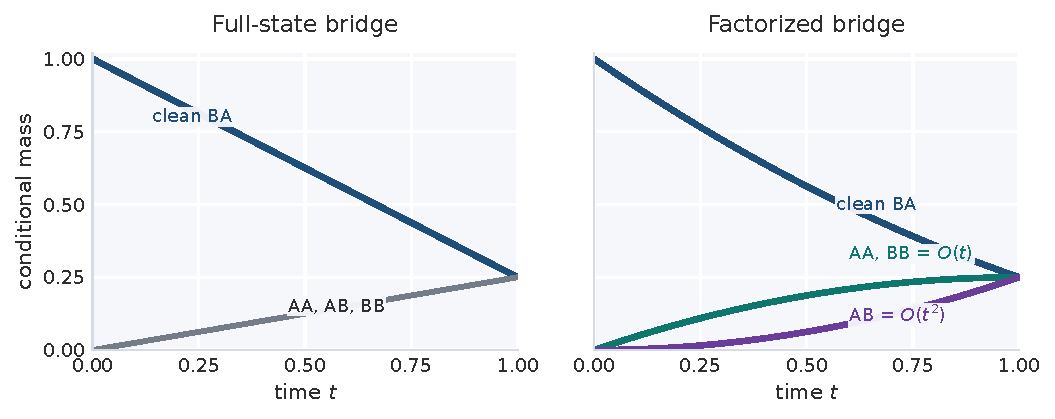
\includegraphics[width=0.92\textwidth]{figures/handouts/discrete_diffusion/fig_discrete_bridge_probabilities}
  \caption{Condition on the current bridge state \texttt{BA} in a two-token binary example.
  Under the exact full-state bridge, the alternative endpoint sequences \texttt{AA}, \texttt{AB}, and \texttt{BB} all enter at first order because one bridge time controls the whole sequence.
  Under the factorized bridge, \texttt{AA} and \texttt{BB} require one backward switch, while \texttt{AB} requires two independent switches and therefore appears only at second order.}
  \label{fig:full-vs-factorized-probabilities}
\end{figure}

This two-token toy calculation is the cleanest reason that coordinatewise marginals become sufficient after factorization.
The same distinction becomes more geometric on the two-dimensional ring example from the diffusion-models unit once we discretize the plane to a grid.
Bin the ring-mixture data law onto that grid, discretize the Gaussian reference law coordinatewise, and apply the factorized bridge \eqref{eq:factorized-mixture-path}.
At the level of marginals we still see the same kind of interpolation from the data endpoint law to the reference endpoint law.
The difference is in the sample-path geometry: the bridge no longer traces a Euclidean curve, and it instead moves by coordinatewise jumps between grid cells.

\begin{figure}[t]
  \centering
  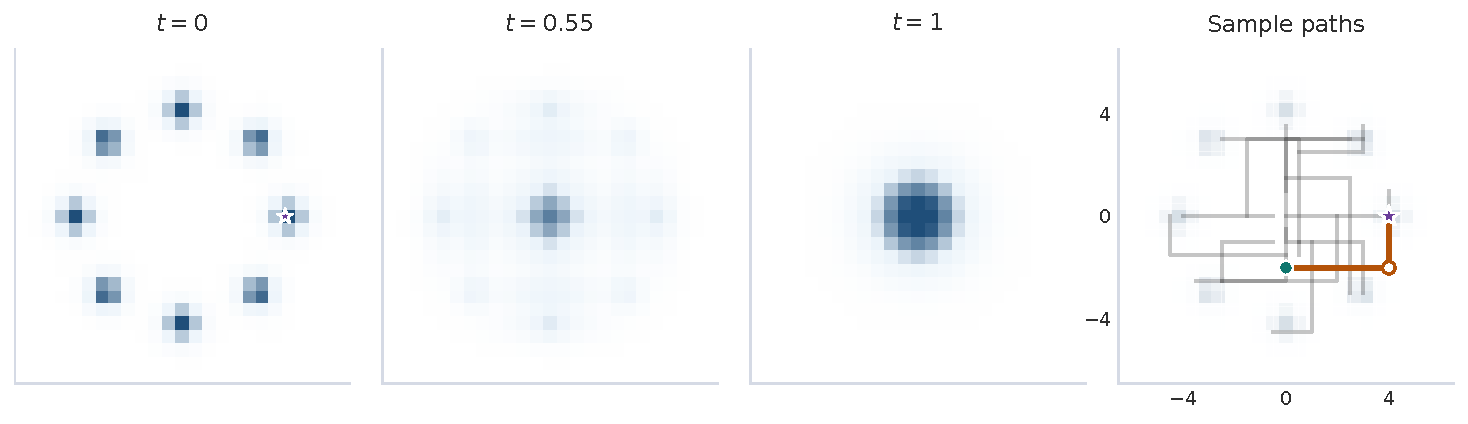
\includegraphics[width=\textwidth]{figures/handouts/discrete_diffusion/fig_discrete_spatial_bridge}
  \caption{A discretized version of the two-dimensional ring-mixture bridge.
  The first three panels show the bridge marginals on the grid at \(t=0\), \(t=0.55\), and \(t=1\).
  The last panel shows sample paths of the factorized bridge; the highlighted path starts from the starred data cell and ends at the teal reference draw.
  The marginal bridge still interpolates between the same endpoint laws, but individual paths move by one-coordinate jumps.}
  \label{fig:discrete-spatial-bridge}
\end{figure}

This is the discrete counterpart of the expectation-based picture in the continuous-state part of the diffusion-models unit.
There one learns a conditional expectation and reads off a velocity field on \(\R^2\).
Here the same bridge logic produces local jump intensities instead of a spatial vector field, which is why the finite-state description naturally passes through a generator.

For a sequence \(x\in\mathcal{V}^d\), let \(x^{j\to v}\) denote the neighbor obtained by replacing coordinate \(j\) by token \(v\).
The endpoint-conditioned generator is then as simple as possible.

\begin{proposition}[Endpoint-conditioned backward switch rule for the factorized bridge]
\label{prop:factorized-conditional-generator}
Let \(c_t\coloneqq -\dot\alpha_t/(1-\alpha_t)\), and assume \(0<\alpha_t<1\).
Then for every single-token neighbor \(x^{j\to v}\),
\begin{equation}
  Q_t^{x_0}\!\bigl(x^{j\to v}\mid x\bigr)
  =
  c_t\,\mathbf{1}\{v=x_{0,j}\}\,\mathbf{1}\{x_j\neq x_{0,j}\},
  \label{eq:factorized-conditional-generator}
\end{equation}
with diagonal chosen so that \(\sum_y Q_t^{x_0}(y\mid x)=0\).
\end{proposition}
\begin{proof}
Fix \(x_0\) and \(x\), and use the coordinatewise coupling \eqref{eq:factorized-coupling}.
If \(x_j=x_{0,j}\), then stepping backward does not require any change at coordinate \(j\).
If \(x_j\neq x_{0,j}\), conditioning on \(X_0=x_0\) and \(X_t=x\) forces \(\tau_j\le t\) and \(\Xi_j=x_j\), and the coordinate switches back exactly when \(\tau_j\in(t-h,t]\).
Therefore
\[
  \mathbb{P}(X_{t-h,j}=x_{0,j}\mid X_0=x_0,X_t=x, x_j\neq x_{0,j})
  =
  \frac{\alpha_{t-h}-\alpha_t}{1-\alpha_t}
  =
  hc_t+o(h).
\]
Independence of the switch times implies that simultaneous switches of two distinct coordinates are \(O(h^2)\), so they disappear at generator scale.
The only off-diagonal first-order moves are the backward switches in \eqref{eq:factorized-conditional-generator}.%
\end{proof}

To pass from the endpoint-conditioned generator to the marginal generator, we use the same posterior-averaging step as in the diffusion-models unit.

\begin{proposition}[Generator-level marginalization on a finite state space]
\label{prop:generator-marginalization}
Suppose
\[
  K_{t-h\mid t}(y\mid x)
  =
  \delta_x(y)+hQ_t(y\mid x)+o(h)
\]
and
\[
  K^{x_0}_{t-h\mid t}(y\mid x)
  =
  \delta_x(y)+hQ_t^{x_0}(y\mid x)+o(h)
\]
as \(h\downarrow 0\).
Then
\[
  Q_t(y\mid x)
  =
  \sum_{x_0\in S} Q_t^{x_0}(y\mid x)\,q_{0\mid t}(x_0\mid x).
\]
\end{proposition}
\begin{proof}
Apply \Cref{prop:finite-state-kernel-marginalization} with \(s=t-h\), insert the first-order expansions, subtract the common zeroth-order term \(\delta_x(y)\), divide by \(h\), and let \(h\downarrow 0\).%
\end{proof}

\begin{theorem}[Factorized generator rates depend only on coordinate marginals]
\label{thm:factorized-rates}
For the factorized mixture path \eqref{eq:factorized-mixture-path}, every off-diagonal single-token jump satisfies
\begin{equation}
  Q_t\!\bigl(x^{j\to v}\mid x\bigr)
  =
  c_t\,q_{0\mid t}\!\bigl(X_{0,j}=v\mid X_t=x\bigr),
  \qquad v\neq x_j.
  \label{eq:factorized-rate}
\end{equation}
\end{theorem}
\begin{proof}
Combine \Cref{prop:generator-marginalization} and \Cref{prop:factorized-conditional-generator}:
\[
  Q_t\!\bigl(x^{j\to v}\mid x\bigr)
  =
  \sum_{x_0\in S}
  c_t\,\mathbf{1}\{x_{0,j}=v\}\,\mathbf{1}\{x_j\neq x_{0,j}\}\,
  q_{0\mid t}(x_0\mid x).
\]
If \(v\neq x_j\), then the second indicator is automatically one on the event \(\{x_{0,j}=v\}\), so
\[
  Q_t\!\bigl(x^{j\to v}\mid x\bigr)
  =
  c_t\sum_{x_0\in S}\mathbf{1}\{x_{0,j}=v\}\,q_{0\mid t}(x_0\mid x)
  =
  c_t\,q_{0\mid t}(X_{0,j}=v\mid X_t=x).
\]
\end{proof}

If we write
\[
  \mu_{t,j}(x)\coloneqq \E[e_{X_{0,j}}\mid X_t=x]\in\R^{|\mathcal{V}|},
\]
then \Cref{thm:factorized-rates} becomes
\begin{equation}
  Q_t\!\bigl(x^{j\to v}\mid x\bigr)
  =
  c_t\,\mu_{t,j}(x)_v,
  \qquad v\neq x_j.
  \label{eq:factorized-rate-onehot}
\end{equation}
This is the cleanest statement of the simplification.
The full posterior over endpoint sequences has not disappeared.
It is still the exact posterior \(q_{0\mid t}(x_0\mid x)\) of the factorized bridge.
What the factorized bridge changes is the local move set: once only one-token backward switches are allowed at first order, the reverse rates query that posterior only through one-coordinate marginals.
So the approximation is in the bridge geometry, not in the posterior-averaging principle.
This is the generator-level reason that tokenwise classification becomes the practical training target.
The next theorem makes that precise: once the factorized bridge has been chosen, exact coordinate posteriors recover its exact reverse generator.

The full-state theorem above says that exact reverse kernels recover the correct law on any time grid.
For the factorized bridge, the parallel statement is now infinitesimal:
an ideal coordinatewise posterior model recovers the exact reverse generator of the chosen factorized bridge.
Recovering the corresponding marginal path on a time grid is then a separate numerical question, handled below by a bound in terms of accumulated one-step kernel error.

\begin{proposition}[Reverse Kolmogorov equation on a finite state space]
\label{prop:reverse-kolmogorov}
Let \(S\) be finite, let \(\pi_t\) be a differentiable path of probability mass functions on \(S\), and let \(Q_t\) be rate matrices whose entries depend continuously on \(t\).
Then the short-time relation
\[
  \pi_{t-h}(y)
  =
  \sum_{x\in S}
  \pi_t(x)\bigl[\delta_x(y)+hQ_t(y\mid x)\bigr]
  +o(h)
\]
for every \(y\in S\) is equivalent to the reverse Kolmogorov equation
\[
  -\frac{d}{dt}\pi_t(y)
  =
  \sum_{x\in S}
  \pi_t(x)\,Q_t(y\mid x),
  \qquad y\in S.
\]
Given the terminal condition \(\pi_1\), this linear ODE has a unique solution.
\end{proposition}
\begin{proof}
Because \(\sum_x \pi_t(x)\delta_x(y)=\pi_t(y)\), the short-time relation is
\[
  \pi_{t-h}(y)
  =
  \pi_t(y)
  +
  h\sum_{x\in S}\pi_t(x)\,Q_t(y\mid x)
  +
  o(h).
\]
Subtract \(\pi_t(y)\), divide by \(h\), and let \(h\downarrow 0\) to obtain the reverse Kolmogorov equation.
Conversely, if the reverse Kolmogorov equation holds, then differentiability gives
\[
  \pi_{t-h}(y)
  =
  \pi_t(y)-h\dot\pi_t(y)+o(h)
  =
  \pi_t(y)
  +
  h\sum_{x\in S}\pi_t(x)\,Q_t(y\mid x)
  +
  o(h),
\]
which is the short-time relation.
Uniqueness follows because this is a linear ODE on the finite-dimensional space \(\R^{|S|}\).%
\end{proof}

\begin{theorem}[Exact coordinate posteriors recover the factorized reverse generator]
\label{thm:factorized-infinitesimal-exactness}
For the factorized mixture path \eqref{eq:factorized-mixture-path}, suppose a model returns the exact coordinate marginals
\[
  \rho_{t,j}^\star(v\mid x)
  =
  q_{0\mid t}(X_{0,j}=v\mid X_t=x).
\]
Define the learned generator by
\[
  \hat Q_t^\star\!\bigl(x^{j\to v}\mid x\bigr)
  \coloneqq
  c_t\,\rho_{t,j}^\star(v\mid x),
  \qquad v\neq x_j,
\]
with diagonal chosen so that \(\sum_y \hat Q_t^\star(y\mid x)=0\).
Then \(\hat Q_t^\star=Q_t\), where \(Q_t\) is the exact reverse generator of the factorized bridge.
Consequently the factorized marginal path \(p_t\) is the unique solution of
\[
  -\frac{d}{dt}p_t(y)
  =
  \sum_{x\in S} p_t(x)\,\hat Q_t^\star(y\mid x),
  \qquad
  p_1 \text{ fixed},
\]
so the exact reverse CTMC for the factorized bridge transports the factorized marginal path back to \(p_0\).
\end{theorem}
\begin{proof}
The equality \(\hat Q_t^\star=Q_t\) is exactly \Cref{thm:factorized-rates}.
Because \(Q_t\) is the exact reverse generator of the factorized bridge,
\[
  K_{t-h\mid t}(y\mid x)
  =
  \delta_x(y)+hQ_t(y\mid x)+o(h).
\]
Combining this with \Cref{prop:reverse-kernels-transport} gives
\[
  p_{t-h}(y)
  =
  \sum_{x\in S}
  p_t(x)\bigl[\delta_x(y)+hQ_t(y\mid x)\bigr]
  +o(h).
\]
By \Cref{prop:reverse-kolmogorov}, the path \(p_t\) therefore solves the reverse Kolmogorov equation with generator \(Q_t=\hat Q_t^\star\).
Uniqueness gives the claim.%
\end{proof}

At this point the modeling approximation is fully visible.
The full-state sequence model and the factorized sequence model are different bridges, so they have different posteriors and different intermediate marginals.
But once the factorized bridge is chosen, \Cref{thm:factorized-infinitesimal-exactness} says that exact coordinate posteriors recover its exact reverse generator.
Equivalently, within the factorized model class the marginal dynamics are completely identified by the coordinate posteriors.
The remaining approximation is then only numerical: how accurately a discrete-time sampler tracks that reverse CTMC.

The exactness theorem above identifies the practical target immediately.
Inside the factorized bridge, learning the reverse dynamics means learning the coordinatewise posterior marginals that determine the reverse rates.
A network \(\rho_t^\theta\) therefore takes a current bridge state \(x\) and time \(t\) and outputs
\[
  \rho_{t,j}^\theta(v\mid x)
  \approx
  q_{0\mid t}(X_{0,j}=v\mid X_t=x).
\]
These outputs are still posterior objects: the full vector \(\mu_t(x)\) in the one-token case and the coordinatewise vectors \(\mu_{t,j}(x)\) in the factorized sequence case.
The statistical question is whether \(\rho_t^\theta\) learns the correct marginals.
The numerical question, which enters only after the model is trained, is how accurately a discrete-time sampler tracks the reverse CTMC determined by those marginals.
Tokenwise cross-entropy addresses the first question.

\begin{proposition}[Cross-entropy is the proper factorized objective]
\label{prop:cross-entropy-proper}
Fix \(t,x,j\), and write
\[
  \pi_j(v)\coloneqq q_{0\mid t}(X_{0,j}=v\mid X_t=x).
\]
For any candidate categorical distribution \(\rho(v)\),
\[
  \E_{V\sim \pi_j}[-\log \rho(V)]
  =
  H(\pi_j)+\operatorname{KL}(\pi_j\|\rho).
\]
Hence the expected tokenwise negative log-likelihood is minimized uniquely at \(\rho=\pi_j\).
\end{proposition}
\begin{proof}
Expand the expectation and add/subtract \(\log \pi_j(v)\):
\[
  \E_{V\sim \pi_j}[-\log \rho(V)]
  =
  \sum_v \pi_j(v)\log\frac{\pi_j(v)}{\rho(v)}
  -
  \sum_v \pi_j(v)\log \pi_j(v)
  =
  \operatorname{KL}(\pi_j\|\rho)+H(\pi_j).
\]
Only the KL term depends on \(\rho\), and it is minimized uniquely when \(\rho=\pi_j\).%
\end{proof}

The corresponding training loss is
\begin{equation}
  \mathcal{L}_{\mathrm{disc}}(\theta)
  =
  \E_{X_0\sim p_0,\; X_t\sim K_{t\mid 0}(\cdot\mid X_0),\; t\sim \mathrm{Unif}[0,1]}
  \left[
    \sum_{j=1}^d
    -\log \rho_{t,j}^\theta(X_{0,j}\mid X_t)
  \right],
  \label{eq:discrete-classification-loss}
\end{equation}
which is exactly the discrete flow-matching objective used by \citet[Eq.~(28) and Prop.~5]{gat2024discrete}.
So classification is not an extra heuristic layered on top of the bridge picture.
It is the proper scoring rule for the posterior statistics that the factorized generator actually needs.
It therefore gives the training loop directly.

\begin{algorithm}[H]
  \caption{Training a factorized discrete diffusion model}
  \label{alg:discrete-diffusion-training}
  \begin{algorithmic}[1]
    \Require Data sampler for \(p_0\), base marginals \(r_1,\dots,r_d\), schedule \(\alpha_t\), posterior network \(\rho_t^\theta\)
    \For{training steps}
      \State Sample \(x_0\sim p_0\) and \(t\sim \mathrm{Unif}[0,1]\)
      \For{\(j=1,\dots,d\) in parallel}
        \State Sample \(B_j\sim \mathrm{Bernoulli}(\alpha_t)\) and \(\Xi_j\sim r_j\)
        \If{\(B_j=1\)}
          \State Set \(x_{t,j}\gets x_{0,j}\)
        \Else
          \State Set \(x_{t,j}\gets \Xi_j\)
        \EndIf
      \EndFor
      \State Form \(x_t=(x_{t,1},\dots,x_{t,d})\)
      \State Evaluate \(\rho_{t,j}^\theta(\cdot\mid x_t)\) for all \(j\)
      \State Compute \(\ell\gets \sum_{j=1}^d -\log \rho_{t,j}^\theta(x_{0,j}\mid x_t)\)
      \State Take a gradient step on \(\ell\)
    \EndFor
  \end{algorithmic}
\end{algorithm}

Once \(\rho_t^\theta\) is trained, we obtain an approximate generator by
\[
  \hat Q_t^\theta(x^{j\to v}\mid x)
  =
  c_t\,\rho_{t,j}^\theta(v\mid x),
  \qquad v\neq x_j.
\]
An exact simulator would sample a CTMC from this generator.
For intuition, the simplest approximation is a parallel Euler step, which keeps the \(O(h)\) single-token events and ignores the \(O(h^2)\) simultaneous jumps over a step of size \(h\).

\begin{algorithm}[H]
  \caption{Euler sampling for the learned CTMC}
  \label{alg:discrete-diffusion-sampling}
  \begin{algorithmic}[1]
    \Require Base sampler for \(p_1\), time grid \(1=t_K>\cdots>t_0=0\), schedule factor \(c_t\), learned posterior network \(\rho_t^\theta\)
    \State Sample \(X_{t_K}\sim p_1\)
    \For{\(k=K,K-1,\dots,1\)}
      \State Set \(t\gets t_k\), \(h\gets t_k-t_{k-1}\), \(x\gets X_{t_k}\)
      \State Evaluate \(\rho_{t,j}^\theta(\cdot\mid x)\) for all coordinates \(j\)
      \For{\(j=1,\dots,d\) in parallel}
        \For{each \(v\neq x_j\)}
          \State \(\tilde p_j(v\mid x_j)\gets h\,c_t\,\rho_{t,j}^\theta(v\mid x)\)
        \EndFor
        \State \(\tilde p_j(x_j\mid x_j)\gets 1-h\sum_{v\neq x_j} c_t\,\rho_{t,j}^\theta(v\mid x)\)
        \State Sample \(X_{t_{k-1},j}\sim \mathrm{Categorical}(\tilde p_j(\cdot\mid x_j))\)
      \EndFor
      \State Set \(X_{t_{k-1}}\gets (X_{t_{k-1},1},\dots,X_{t_{k-1},d})\)
    \EndFor
    \State \Return \(X_{t_0}\)
  \end{algorithmic}
\end{algorithm}

Euler is only the time discretization.
The structural approximation happened earlier, when we replaced the full \(|\mathcal{V}|^d\)-state model by the factorized local bridge.
That distinction matters because classification is learning the posterior statistics needed by the chosen local generator, while Euler is only approximating the CTMC generated by those statistics.
For the per-coordinate categorical probabilities in \Cref{alg:discrete-diffusion-sampling} to be valid, we choose a grid fine enough that
\[
  h\,c_t\le 1
\]
at every step; this guarantees \(\tilde p_j(x_j\mid x_j)\ge 0\).
With that understood, the Euler sampler is one concrete family of approximate kernels \(\hat K_k\).

This isolates the remaining numerical question.
Fix a time grid and let \(K_k=K_{t_{k-1}\mid t_k}\) denote the exact reverse kernels of the factorized bridge on that grid.
Any practical sampler, including \Cref{alg:discrete-diffusion-sampling}, replaces \(K_k\) by approximate kernels \(\hat K_k\).
The only question is how those one-step kernel errors accumulate.

\begin{proposition}[Accumulated one-step kernel error controls gridwise marginal error]
\label{prop:accumulated-kernel-error}
Fix a decreasing grid \(1=t_K>\cdots>t_0=0\).
Let \(K_k=K_{t_{k-1}\mid t_k}\) be the exact reverse kernels of a bridge path, and let \(\hat K_k\) be any approximate reverse kernels on the same grid.
Start both chains from the same terminal law,
\[
  p_K=\hat p_K=p_1,
\]
and define
\[
  p_{k-1}=p_k K_k,
  \qquad
  \hat p_{k-1}=\hat p_k \hat K_k,
  \qquad k=K,\dots,1.
\]
For each step set
\[
  \varepsilon_k
  \coloneqq
  \sup_{x\in S}
  \sum_{y\in S}
  \bigl|\hat K_k(y\mid x)-K_k(y\mid x)\bigr|.
\]
Then for every \(m=0,\dots,K\),
\[
  \|\hat p_m-p_m\|_1
  \le
  \sum_{k=m+1}^K \varepsilon_k.
\]
In particular,
\[
  \|\hat p_0-p_0\|_1
  \le
  \sum_{k=1}^K \varepsilon_k.
\]
\end{proposition}
\begin{proof}
If \(m\) is any signed mass function on \(S\) and \(K\) is any Markov kernel, then
\[
  \|mK\|_1
  =
  \sum_{y\in S}
  \left|\sum_{x\in S} m(x)\,K(y\mid x)\right|
  \le
  \sum_{x\in S}|m(x)|\sum_{y\in S}K(y\mid x)
  =
  \|m\|_1.
\]
So Markov kernels are \(\ell_1\)-contractive.
Now
\[
  \hat p_{k-1}-p_{k-1}
  =
  (\hat p_k-p_k)\hat K_k
  +
  p_k(\hat K_k-K_k),
\]
and therefore
\[
  \|\hat p_{k-1}-p_{k-1}\|_1
  \le
  \|(\hat p_k-p_k)\hat K_k\|_1
  +
  \|p_k(\hat K_k-K_k)\|_1
  \le
  \|\hat p_k-p_k\|_1+\varepsilon_k.
\]
Iterating backward from \(\|\hat p_K-p_K\|_1=0\) gives the stated bound for every grid point.%
\end{proof}

\begin{corollary}[Small-step recovery of the factorized marginal path]
\label{cor:factorized-small-step-recovery}
Consider the factorized bridge \eqref{eq:factorized-mixture-path}, and suppose the learned posterior model is ideal so that \(\rho_{t,j}^\star(v\mid x)=q_{0\mid t}(X_{0,j}=v\mid X_t=x)\).
For each grid \(\Pi^{(n)}=\{1=t^{(n)}_{K_n}>\cdots>t^{(n)}_0=0\}\), let \(K_k^{(n)}\) be the exact reverse kernels of the factorized bridge and let \(\hat K_k^{(n)}\) be any approximate kernels built from those exact coordinate marginals.
If
\[
  \sum_{k=1}^{K_n}
  \sup_{x\in S}\sum_{y\in S}
  \bigl|\hat K_k^{(n)}(y\mid x)-K_k^{(n)}(y\mid x)\bigr|
  \longrightarrow 0
  \qquad\text{as } n\to\infty,
\]
then the approximate reverse chain converges at every grid point to the marginal path of the factorized bridge.
In particular,
\[
  \|\hat p_0^{(n)}-p_0\|_1\to 0.
\]
\end{corollary}
\begin{proof}
By \Cref{thm:factorized-infinitesimal-exactness}, the exact coordinate marginals recover the exact reverse generator of the factorized bridge.
Hence the exact reverse kernels \(K_k^{(n)}\) are the correct kernels for that bridge on the grid \(\Pi^{(n)}\).
Applying \Cref{prop:accumulated-kernel-error} to each grid gives the result.%
\end{proof}

This is the precise sense in which the practical factorized sampler becomes exact.
It does not say that the factorized bridge reproduces the exact full-state bridge on \(\mathcal{V}^d\); that modeling approximation was made earlier.
It says that once the factorized bridge is chosen, exact coordinate posteriors plus vanishing one-step kernel error recover its marginal path, and therefore its data endpoint \(p_0\), in the many-step limit.

\begin{exercise}[Reading factorized reverse rates]
\label{ex:reading-factorized-rates}
Stay inside the factorized bridge on the binary vocabulary \(\mathcal{V}=\{A,B\}\), and let the current bridge state be \(x=\texttt{BA}\).
Suppose
\[
  q_{0\mid t}(X_{0,1}=A\mid X_t=x)=0.6,
  \qquad
  q_{0\mid t}(X_{0,1}=B\mid X_t=x)=0.4,
\]
\[
  q_{0\mid t}(X_{0,2}=A\mid X_t=x)=0.2,
  \qquad
  q_{0\mid t}(X_{0,2}=B\mid X_t=x)=0.8,
\]
and \(c_t=3\).
\begin{enumerate}[leftmargin=*]
  \item Compute the off-diagonal reverse rates from \(\texttt{BA}\) to \(\texttt{AA}\) and to \(\texttt{BB}\).
  \item Compute the diagonal entry \(Q_t(\texttt{BA}\mid \texttt{BA})\).
  \item Explain why no table of joint probabilities \(q_{0\mid t}(X_{0,1},X_{0,2}\mid X_t=x)\) appears in these rates.
\end{enumerate}
\end{exercise}
\SolutionBox[10]{The neighbor \(\texttt{AA}\) is \(x^{1\to A}\), so \eqref{eq:factorized-rate} gives
\[
  Q_t(\texttt{AA}\mid \texttt{BA})
  =
  3\cdot q_{0\mid t}(X_{0,1}=A\mid X_t=x)
  =
  3(0.6)
  =
  1.8.
\]
Similarly \(\texttt{BB}=x^{2\to B}\), so
\[
  Q_t(\texttt{BB}\mid \texttt{BA})
  =
  3\cdot q_{0\mid t}(X_{0,2}=B\mid X_t=x)
  =
  3(0.8)
  =
  2.4.
\]
The row sum must vanish, hence
\[
  Q_t(\texttt{BA}\mid \texttt{BA})=-(1.8+2.4)=-4.2.
\]
No joint two-token table appears because the factorized bridge only allows one-token backward switches at first order.
Once the local move set is restricted to \(x^{j\to v}\), the reverse generator queries the posterior only through one-coordinate marginals.}

\begin{exercise}[Why only one-token jumps survive at first order]
\label{ex:one-token-jumps}
Use the factorized coupling \eqref{eq:factorized-coupling}.
Fix two distinct coordinates \(j\neq k\), and suppose both are currently away from their \(t=0\) endpoint values, so \(x_j\neq x_{0,j}\) and \(x_k\neq x_{0,k}\).
\begin{enumerate}[leftmargin=*]
  \item Show that
  \[
    \mathbb{P}\bigl(X_{t-h,j}=x_{0,j},\,X_{t-h,k}=x_{0,k}\mid X_0=x_0,\;X_t=x\bigr)
    =
    O(h^2).
  \]
  \item Explain why this implies that two-token jumps disappear at generator scale.
  \item Conclude that the generator-level reverse object only needs the coordinate marginals \(q_{0\mid t}(X_{0,j}=v\mid X_t=x)\), not simultaneous two-token switch probabilities.
\end{enumerate}
\end{exercise}
\SolutionBox[12]{Conditionally on \(X_0=x_0\) and \(X_t=x\), each coordinate that is away from its \(t=0\) endpoint switches back exactly when its switch time lies in \((t-h,t]\).
For one coordinate this has probability
\[
  \mathbb{P}(\tau_j\in (t-h,t]\mid \tau_j\le t)
  =
  hc_t+o(h).
\]
Because the switch times are independent across coordinates,
\begin{align*}
  &\mathbb{P}\bigl(X_{t-h,j}=x_{0,j},\,X_{t-h,k}=x_{0,k}\mid X_0=x_0,\;X_t=x\bigr) \\
  &\qquad=
  \mathbb{P}(\tau_j\in (t-h,t]\mid \tau_j\le t)\,
  \mathbb{P}(\tau_k\in (t-h,t]\mid \tau_k\le t)
  =
  \bigl(hc_t+o(h)\bigr)^2
  =
  O(h^2).
\end{align*}
After dividing by \(h\) to form the generator, any \(O(h^2)\) event vanishes.
So the first-order reverse dynamics can only move along one-token neighbors.
That is the structural reason the generator depends only on one-coordinate posterior marginals: simultaneous two-token switch probabilities never appear at first order.}

\subsection{Masked diffusion as a sharpened special case}
\label{subsec:masked-diffusion}

Masked diffusion makes the factorized story even cleaner by collapsing the reference law to a point mass.
It is not a new approximation layer; it is a particularly simple factorized bridge.
Adjoin an absorbing token \([\mathrm{MASK}]\notin\mathcal{V}\), set \(r_j=\delta_{[\mathrm{MASK}]}\) for every coordinate, and let
\[
  p_1=\delta_{[\mathrm{MASK}]^d}.
\]
Each coordinate now either keeps the \(t=0\) endpoint token or is replaced by \([\mathrm{MASK}]\).
Equivalently, the factorized bridge becomes
\begin{equation}
  K_{t\mid 0}(x\mid x_0)
  =
  \prod_{j=1}^d
  \Bigl[
    \alpha_t\,\delta_{x_{0,j}}(x_j)
    +
    (1-\alpha_t)\,\delta_{[\mathrm{MASK}]}(x_j)
  \Bigr].
  \label{eq:masked-factorized-bridge}
\end{equation}
This is the absorbing-mask version of the same factorized bridge picture.

\begin{corollary}[Revealed coordinates are already solved]
\label{cor:masked-revealed}
If \(X_{t,j}\neq [\mathrm{MASK}]\), then
\[
  q_{0\mid t}(X_{0,j}=X_{t,j}\mid X_t)=1
\]
and
\[
  q_{0\mid t}(X_{0,j}=v\mid X_t)=0
  \qquad \text{for } v\neq X_{t,j}.
\]
\end{corollary}
\begin{proof}
Under the masked bridge, a revealed token can only arise by keeping the \(t=0\) endpoint token.
So any endpoint sequence compatible with \(X_t\) must satisfy \(X_{0,j}=X_{t,j}\).%
\end{proof}

The second simplification is specific to the absorbing mask.
Once the current state tells us which coordinates are revealed and which are masked, the schedule factor contributes the same scalar weight to every compatible endpoint sequence.
After normalization it cancels.

\begin{proposition}[The masked posterior does not depend on time]
\label{prop:masked-time-independent}
Let \(x\in(\mathcal{V}\cup\{[\mathrm{MASK}]\})^d\), and define
\[
  U(x)\coloneqq \{j:x_j\neq [\mathrm{MASK}]\},
  \qquad
  M(x)\coloneqq \{j:x_j=[\mathrm{MASK}]\}.
\]
For the masked factorized bridge,
\begin{equation}
  K_{t\mid 0}(x\mid x_0)
  =
  \alpha_t^{|U(x)|}(1-\alpha_t)^{|M(x)|}
  \prod_{j\in U(x)} \mathbf{1}\{x_{0,j}=x_j\}.
  \label{eq:masked-likelihood-factor}
\end{equation}
Consequently,
\begin{equation}
  q_{0\mid t}(x_0\mid x)
  \propto
  p_0(x_0)\prod_{j\in U(x)}\mathbf{1}\{x_{0,j}=x_j\},
  \label{eq:masked-posterior-t-free}
\end{equation}
so the posterior depends on the masked pattern and the revealed tokens, but not on \(t\).
\end{proposition}
\begin{proof}
Each revealed coordinate contributes \(\alpha_t\,\mathbf{1}\{x_{0,j}=x_j\}\), and each masked coordinate contributes \(1-\alpha_t\).
Multiplying over coordinates gives \eqref{eq:masked-likelihood-factor}.
Bayes' rule then yields
\[
  q_{0\mid t}(x_0\mid x)
  \propto
  p_0(x_0)\,\alpha_t^{|U(x)|}(1-\alpha_t)^{|M(x)|}
  \prod_{j\in U(x)}\mathbf{1}\{x_{0,j}=x_j\}.
\]
The schedule factor does not depend on \(x_0\), so it cancels during normalization.%
\end{proof}

Equivalently, once we observe a masked row \(x\), the posterior is just the data law \(p_0\) renormalized on the set of endpoint sequences that agree with the revealed coordinates \(x_{U(x)}\).
The only role of the forward schedule is to contribute the common scalar \(\alpha_t^{|U(x)|}(1-\alpha_t)^{|M(x)|}\), and that scalar disappears when we normalize.

This is the posterior explanation for two familiar implementation choices.
First, the network can ignore time in the purely masked setting because the target posterior is time-independent \citep[Prop.~6 and App.~E.8]{gat2024discrete}.
Second, the loss can be restricted to masked positions because revealed coordinates already have degenerate posteriors.
That is exactly why the absorbing mask collapses the generic bridge problem to ordinary prediction on the masked coordinates.

\begin{exercise}[Why the schedule cancels in the masked case]
\label{ex:masked-cancel}
Fix a masked bridge state \(x\), and let \(U(x)\) and \(M(x)\) denote its revealed and masked coordinates.
\begin{enumerate}[leftmargin=*]
  \item Starting from \eqref{eq:masked-likelihood-factor}, show that every endpoint sequence compatible with the revealed coordinates receives the same factor
  \[
    \alpha_t^{|U(x)|}(1-\alpha_t)^{|M(x)|}.
  \]
  \item Use Bayes' rule to derive \eqref{eq:masked-posterior-t-free}.
  \item For a masked coordinate \(j\in M(x)\), prove that for every token \(v\in\mathcal{V}\),
  \[
    q_{0\mid t}(X_{0,j}=v\mid X_t=x)
    =
    \mathbb{P}_{X_0\sim p_0}\bigl(X_{0,j}=v \mid X_{0,U(x)}=x_{U(x)}\bigr).
  \]
  \item Why can the loss be restricted to masked positions?
\end{enumerate}
\end{exercise}
\SolutionBox[14]{By \eqref{eq:masked-likelihood-factor},
\[
  K_{t\mid 0}(x\mid x_0)
  =
  \alpha_t^{|U(x)|}(1-\alpha_t)^{|M(x)|}
  \prod_{i\in U(x)}\mathbf{1}\{x_{0,i}=x_i\}.
\]
So every endpoint sequence \(x_0\) compatible with the revealed coordinates gets the same schedule-dependent factor, and every incompatible sequence gets likelihood zero.
Bayes' rule gives
\[
  q_{0\mid t}(x_0\mid x)
  \propto
  p_0(x_0)\,
  \alpha_t^{|U(x)|}(1-\alpha_t)^{|M(x)|}
  \prod_{i\in U(x)}\mathbf{1}\{x_{0,i}=x_i\}.
\]
The schedule factor does not depend on \(x_0\), so it cancels during normalization:
\[
  q_{0\mid t}(x_0\mid x)
  \propto
  p_0(x_0)\prod_{i\in U(x)}\mathbf{1}\{x_{0,i}=x_i\}.
\]
Therefore, for \(j\in M(x)\),
\[
  q_{0\mid t}(X_{0,j}=v\mid X_t=x)
  =
  \mathbb{P}_{X_0\sim p_0}\bigl(X_{0,j}=v \mid X_{0,U(x)}=x_{U(x)}\bigr).
\]
Revealed positions can be dropped from the loss because their posteriors are already point masses by \Cref{cor:masked-revealed}; only the masked coordinates still carry uncertainty.}

\subsection{Connection back to the Euclidean expectation lens}
\label{subsec:euclidean-connection}

The bridge-first parallel with the Euclidean setting can be written explicitly:
\[
  \begin{aligned}
    \text{Euclidean bridge:}\qquad
    &\text{learn }
    \E[\dot X_t\mid X_t=x]
    \text{ or }
    \E[X_0\mid X_t=x].\\[0.35em]
    \text{Full finite-state bridge on }S:\qquad
    &\text{learn }
    \E[e_{X_0}\mid X_t=x]
    =
    q_{0\mid t}(\cdot\mid x).\\[0.35em]
    \text{Factorized bridge on }\mathcal{V}^d:\qquad
    &\text{learn }
    \E[e_{X_{0,j}}\mid X_t=x]
    =
    q_{0\mid t}(X_{0,j}=\cdot\mid X_t=x)
    \text{ for each }j.
  \end{aligned}
\]

The Euclidean model cannot represent the full posterior by a finite-dimensional simplex vector, so it learns the conditional expectations under that posterior that are infinitesimally sufficient for the marginal dynamics.
The one-token discrete model can represent the full posterior exactly, because a one-hot expectation on a finite set is already a probability vector.
The factorized sequence model makes the parallel tractability move: it keeps the posterior-averaging principle but chooses a local jump geometry whose infinitesimal rates depend only on coordinatewise posterior marginals.
Within that factorized model, those marginals still recover the correct reverse dynamics and therefore the correct endpoint law \(p_0\).
That is the precise sense in which practical discrete diffusion reduces to classification.

So the clean conclusion is not that discrete diffusion secretly stops being distributional.
It is the opposite.
The exact finite-state story is fully distributional from the start, and tokenwise classification appears only after we decide to approximate the full sequence model by a factorized local bridge.

\begin{exercise}[Classify the bridge]
\label{ex:classify-the-bridge}
For each scenario below, decide whether the tokenwise-classification reduction developed above is exact at the generator level, exact only in the masked/time-independent special case, or only approximate.
In each case, identify the first-order reverse move set and the first model change you would try if that reduction fails.
\begin{enumerate}[leftmargin=*]
  \item A one-token categorical bridge with a known schedule.
  \item A factorized sequence bridge with independent switch times.
  \item A masked bridge where the network is trained only on masked positions.
  \item A coupled bridge in which two-token moves occur at first order.
\end{enumerate}
\end{exercise}
\SolutionBox[14]{For the one-token categorical bridge, classification is exact at the generator level:
the reverse chain can jump from the current token \(x\) to any token \(v\neq x\), and the rates are exactly the posterior coordinates \(q_{0\mid t}(X_0=v\mid X_t=x)\).
For the factorized sequence bridge, classification is again exact at the generator level:
the first-order move set consists of one-token neighbors \(x^{j\to v}\), and the corresponding rates are exactly the coordinate marginals \(q_{0\mid t}(X_{0,j}=v\mid X_t=x)\).
For the masked bridge, this is the masked/time-independent special case of the factorized bridge, so the reduction remains exact at the generator level:
the uncertain moves live only on masked coordinates, the posterior ignores \(t\), and training can therefore be restricted to masked positions whose posteriors are not already degenerate.
For a coupled bridge with two-token moves at first order, classification is only approximate.
The reverse generator now needs block moves or other nonlocal jumps, so a tokenwise classifier is missing the first-order object itself.
The first fix is to enlarge the learned reverse object, for example by modeling blockwise posteriors or a richer reverse kernel that can score coupled edits.}

\subsection{Other discrete variants}
\label{subsec:other-discrete-variants}

The discussion above focused on one model class:
a factorized bridge, its reverse CTMC, and the discrete flow-matching objective that learns the posterior marginals needed by that generator.
That is the cleanest setup for developing the distributional picture without fragmentation.

Other named discrete diffusion models can mostly be understood as changing one of three ingredients while keeping the same bridge-first logic.
The uniform multinomial kernel of \citet[\S4]{hoogeboom2021argmax} is the basic one-token categorical instance of this story.
Absorbing-mask models are the sharpened special case from \Cref{subsec:masked-diffusion}; in discrete time this is the absorbing-state construction in \citet[\S3.1]{austin2021structured}, while in the present flow-matching setup the posterior simplification is exactly the one stated in \citep[Prop.~6 and App.~E.8]{gat2024discrete}.
Richer D3PM-style constructions play the same role by changing the one-token forward corruption kernel in the discrete-time model \citep[\S3.1--3.3]{austin2021structured}; in the bridge-first view used here, that changes the local geometry while leaving the posterior-averaging principle intact.

So the real conceptual distinction is not between many separate algorithms.
It is between the exact full-state bridge, the tractable factorized bridge, and the numerical schemes used to approximate reverse-time sampling once that bridge has been chosen.
Carried back to the main notes, the lesson is the same as in the Euclidean diffusion story: choose a bridge, identify the conditional object that is sufficient for reverse-time transport, and then ask which tractable approximation preserves that sufficiency.
The discrete setting is simply the case where, for some bridges, that conditional object is a literal posterior vector rather than a lower-dimensional summary.

\bibliographystyle{plainnat}
\makeatletter
\begingroup
\let\input@path\@empty
\IfFileExists{references.bib}{%
  \gdef\stat221bibpath{references}%
}{%
  \IfFileExists{../references.bib}{%
    \gdef\stat221bibpath{../references}%
  }{%
    \gdef\stat221bibpath{../../references}%
  }%
}
\endgroup
\makeatother
\bibliography{\stat221bibpath}

\end{document}
"
%   (Low-level direct build: if you invoke latexmk manually, set -jobname to the
%    titled output so the compiled PDF matches the standard naming scheme.)
\newif\ifshowsolutions
\showsolutionsfalse
\ifdefined\STATshowsolutions
  \showsolutionstrue
\fi
\ifcsname STAT221SOLUTIONS\endcsname
  \showsolutionstrue
\fi

% Solutions/workspace boxes (controlled by \ifshowsolutions).
% Usage: \SolutionBox[<workspace lines>]{<solution body>}
\newcommand{\SolutionBox}[2][10]{%
  \ifshowsolutions
    \begin{tcolorbox}[stat221panelgray,title={Solution}]
    #2
    \end{tcolorbox}
  \else
    \begin{tcolorbox}[stat221panelgray,unbreakable,title={Workspace}]
    \vspace{#1\baselineskip}
    \end{tcolorbox}
  \fi
}

\title{Discrete diffusion as posterior learning}
\author{}
\date{}

\begin{document}
\maketitle

\section[Discrete diffusion as posterior learning]{Discrete diffusion as posterior learning}
\label{sec:discrete-posterior-learning}

Fix a finite state space \(S\).
This handout takes the diffusion unit's bridge-first viewpoint and specializes it to a setting where the reverse-time object can sometimes be represented exactly.
The central ingredients are the endpoint laws \(p_0\) and \(p_1\), the chosen bridge \(K_{t\mid 0}(\cdot\mid x_0)\), and the endpoint posterior \(q_{0\mid t}\) induced by that bridge.
In finite state spaces the resulting question becomes unusually clean: when does reverse sampling reduce to classification, and when does tractability require a change in the bridge itself?

Let \(p_0\) be the data law on \(S\), let \(p_1\) be a reference law, and let \(K_{t\mid 0}(\cdot\mid x_0)\) be a conditional probability path with
\[
  K_{0\mid 0}(\cdot\mid x_0)=\delta_{x_0},
  \qquad
  K_{1\mid 0}(\cdot\mid x_0)=p_1.
\]
Averaging over \(X_0\sim p_0\) gives the marginal law \(p_t\), and Bayes' rule gives the endpoint posterior
\[
  q_{0\mid t}(x_0\mid x)
  =
  \frac{p_0(x_0)K_{t\mid 0}(x\mid x_0)}{p_t(x)}.
\]
If we knew this posterior exactly, reverse sampling would be straightforward:
sample an endpoint from \(q_{0\mid t}(\cdot\mid x)\) and then take the bridge step conditioned on that endpoint.
This is the finite-state specialization of the posterior-averaging mechanism developed in the diffusion-models unit.

When \(S\) is small, the one-hot conditional expectation \(\E[e_{X_0}\mid X_t=x]\) is already the full posterior vector \(q_{0\mid t}(\cdot\mid x)\).
For a one-token vocabulary model that means classifier outputs can represent the exact reverse-time object.
For the full sequence state space \(S=\mathcal{V}^d\), the same statement remains true but becomes computationally useless because the simplex has size \(|\mathcal{V}|^d\).
Practical discrete diffusion therefore changes the bridge, not the posterior-averaging principle: it replaces the exact full-sequence bridge by a coordinatewise bridge whose reverse generator depends only on coordinatewise posterior marginals.
The discussion below follows that progression from the exact finite-state bridge to the exact full-sequence model and then to the factorized sequence bridge used in practice.

\subsection{Exact posterior learning on a finite state space}
\label{subsec:finite-state-full-posterior}

We now specialize the bridge and posterior notation of the diffusion-models unit to a finite state space \(S\).
Let \(p_0\) be the data law, \(p_1\) a reference law, and
\[
  K_{t\mid 0}(\cdot\mid x_0),
  \qquad
  K_{0\mid 0}(\cdot\mid x_0)=\delta_{x_0},
  \qquad
  K_{1\mid 0}(\cdot\mid x_0)=p_1
\]
is a conditional probability path.
The corresponding marginal path is
\[
  p_t(x)=\sum_{x_0\in S} p_0(x_0)\,K_{t\mid 0}(x\mid x_0),
\]
and Bayes' rule gives the posterior over the \(t=0\) endpoint states,
\[
  q_{0\mid t}(x_0\mid x)
  =
  \frac{p_0(x_0)K_{t\mid 0}(x\mid x_0)}{p_t(x)}.
\]
This formula is understood on the support of \(p_t\), that is, for states \(x\) with \(p_t(x)>0\).

In the Euclidean development of the diffusion-models unit, one passes from the full posterior to conditional expectations that are infinitesimally sufficient.
On a finite state space, a one-hot embedding of the \(t=0\) endpoint loses no information, so the same conditional expectation is the full posterior itself.
Suppressing the dependence on \(S\), write \(e_z\in\R^{|S|}\) for the basis vector indexed by \(z\in S\).

\begin{proposition}[The one-hot conditional expectation is the full posterior]
\label{prop:full-state-onehot}
Define
\[
  \mu_t(x)\coloneqq \E[e_{X_0}\mid X_t=x]\in\R^{|S|}.
\]
Then
\begin{equation}
  \mu_t(x)_z
  =
  q_{0\mid t}(X_0=z\mid X_t=x),
  \qquad z\in S.
  \label{eq:full-state-onehot}
\end{equation}
\end{proposition}
\begin{proof}
Because \(e_{X_0}=e_z\) on the event \(\{X_0=z\}\),
\[
  \mu_t(x)
  =
  \sum_{z\in S} e_z\,\mathbb{P}(X_0=z\mid X_t=x).
\]
Taking the \(z\)th coordinate gives \eqref{eq:full-state-onehot}.%
\end{proof}

\Cref{prop:full-state-onehot} is the finite-state version of the Euclidean expectation reduction, except that here the reduction is exact.
In Euclidean space, quantities like \(\E[\dot X_t\mid X_t=x]\) or \(\E[X_0\mid X_t=x]\) summarize a richer posterior.
For a finite state space, the one-hot expectation \(\E[e_{X_0}\mid X_t=x]\) already is the posterior.
When \(S=\mathcal{V}\), a classifier over the vocabulary is therefore an exact posterior model.

\begin{figure}[t]
  \centering
  \begin{tikzpicture}[font=\small]
  \tikzset{
    panel/.style={
      rounded corners=7pt,
      draw=stat221Gray!30,
      fill=stat221GrayLight,
      line width=0.85pt,
    },
    infobox/.style={
      rounded corners=5pt,
      draw=stat221Blue!55!black,
      fill=white,
      line width=0.85pt,
      inner sep=8pt,
      text width=4.6cm,
      align=left,
    },
    coordlabel/.style={
      font=\footnotesize,
      fill=white,
      inner sep=1.5pt,
      text=stat221Gray,
    },
  }

  \path[use as bounding box] (-0.1,-0.1) rectangle (13.9,5.25);
  \draw[panel] (0,0) rectangle (13.7,4.95);

  \node[font=\small\bfseries,text=stat221Gray] at (3.10,4.58)
    {The posterior lives in the simplex};
  \node[font=\small\bfseries,text=stat221Gray] at (10.28,4.58)
    {Its coordinates are the reverse rates};

  \coordinate (A) at (0.95,0.78);
  \coordinate (B) at (5.85,0.78);
  \coordinate (C) at (3.40,3.95);
  \coordinate (P) at (2.76,1.50);

  \fill[white] (A) -- (B) -- (C) -- cycle;
  \draw[stat221Gray!70,line width=1.05pt] (A) -- (B) -- (C) -- cycle;

  % Constant-coordinate lines through the posterior point.
  \draw[stat221Blue!70!black,densely dashed,line width=1.0pt]
    ($(A)!0.5!(B)$) -- ($(A)!0.5!(C)$);
  \draw[stat221Green!70!black,densely dashed,line width=1.0pt]
    ($(B)!0.3!(A)$) -- ($(B)!0.3!(C)$);
  \draw[stat221Purple!70!black,densely dashed,line width=1.0pt]
    ($(C)!0.2!(A)$) -- ($(C)!0.2!(B)$);

  \filldraw[fill=stat221BlueLight,draw=stat221Blue!70!black,line width=0.9pt] (A) circle (0.16);
  \filldraw[fill=stat221GreenLight,draw=stat221Green!70!black,line width=0.9pt] (B) circle (0.16);
  \filldraw[fill=stat221PurpleLight,draw=stat221Purple!70!black,line width=0.9pt] (C) circle (0.16);
  \node[font=\small\bfseries,text=stat221Blue!75!black] at ($(A)+(-0.38,-0.28)$) {\(A\)};
  \node[font=\small\bfseries,text=stat221Green!60!black] at ($(B)+(0.38,-0.28)$) {\(B\)};
  \node[font=\small\bfseries,text=stat221Purple!60!black] at ($(C)+(0.00,0.35)$) {\(C\)};

  \filldraw[fill=stat221Gray,draw=white,line width=0.9pt] (P) circle (0.12);
  \draw[stat221Gray!60,line width=0.8pt] (P) -- +(0.55,0.55);
  \node[font=\small,text=stat221Gray,align=left] at ($(P)+(0.68,0.68)$)
    {\(\mu_t(x)\)};
  \node[font=\scriptsize,text=stat221Gray,align=left] at ($(P)+(0.92,0.28)$)
    {\(=q_{0\mid t}(\cdot\mid x)\)};

  \node[coordlabel,text=stat221Blue!75!black] at (1.80,2.38) {\(A=0.5\)};
  \node[coordlabel,text=stat221Green!60!black] at (4.85,2.10) {\(B=0.3\)};
  \node[coordlabel,text=stat221Purple!60!black] at (2.35,1.02) {\(C=0.2\)};

  \node[infobox] (info) at (10.30,2.45) {%
    \(\displaystyle \mu_t(x)=(0.5,\,0.3,\,0.2)\)

    \vspace{0.45em}
    \textcolor{stat221Blue!75!black}{\(Q_t^{\mathrm{rev}}(A\mid x)=0.5\,c_t\)}

    \textcolor{stat221Green!60!black}{\(Q_t^{\mathrm{rev}}(B\mid x)=0.3\,c_t\)}

    \textcolor{stat221Purple!60!black}{\(Q_t^{\mathrm{rev}}(C\mid x)=0.2\,c_t\)}

    \vspace{0.55em}
    The reverse generator is \(c_t\) times these coordinates.};
\end{tikzpicture}

  \caption{In the one-token setting, the posterior is literally a point in the simplex over endpoint states.
  Learning that point is genuinely distributional, and the reverse generator just rescales its coordinates by the common jump rate \(c_t\).}
  \label{fig:one-token-distributional}
\end{figure}

This is the discrete analogue of the conditional-versus-marginal story in the diffusion-models unit.
We observe the current bridge state \(X_t=x\), infer the conditional law of the endpoint \(X_0\mid X_t=x\), and then use a sampled endpoint to take the reverse bridge step.
The only difference from the Euclidean case is that on a finite set the relevant posterior can sometimes be represented exactly by a finite vector.

Operationally, an exact finite-state bridge can therefore be sampled in two stages.
Given a current state \(x_t\) and an earlier time \(s<t\), first draw an endpoint and then draw from the bridge conditioned on that endpoint:
\[
  \tilde X_0\sim q_{0\mid t}(\cdot\mid x_t),
  \qquad
  X_s\sim K^{\tilde X_0}_{s\mid t}(\cdot\mid x_t).
\]
Marginalizing \(\tilde X_0\) recovers the exact earlier-time kernel \(K_{s\mid t}(\cdot\mid x_t)\).
So in the one-token case there is no approximation to explain away: infer the full conditional law of \(X_0\mid X_t=x_t\), sample an endpoint from it, and then take the exact bridge step conditioned on that sample.

\begin{proposition}[Endpoint-conditioned bridge marginalization on a finite state space]
\label{prop:finite-state-kernel-marginalization}
Let \(0\le s\le t\le 1\).
Write \(K^{x_0}_{s\mid t}(\cdot\mid x_t)\) for the bridge kernel from time \(t\) to the earlier time \(s\) conditioned on the endpoint \(X_0=x_0\).
Then
\[
  K_{s\mid t}(y\mid x_t)
  =
  \sum_{x_0\in S}
  K^{x_0}_{s\mid t}(y\mid x_t)\,
  q_{0\mid t}(x_0\mid x_t).
\]
\end{proposition}
\begin{proof}
For states \(x_t\) with \(p_t(x_t)>0\), the law of total probability gives
\[
  \mathbb{P}(X_s=y\mid X_t=x_t)
  =
  \sum_{x_0\in S}
  \mathbb{P}(X_s=y\mid X_0=x_0,X_t=x_t)\,
  \mathbb{P}(X_0=x_0\mid X_t=x_t).
\]
This is exactly the displayed identity.%
\end{proof}

\begin{proposition}[Exact reverse kernels transport the marginal path]
\label{prop:reverse-kernels-transport}
For every \(0\le s\le t\le 1\),
\[
  p_s(y)
  =
  \sum_{x\in S} p_t(x)\,K_{s\mid t}(y\mid x),
  \qquad y\in S.
\]
\end{proposition}
\begin{proof}
Again by the law of total probability,
\[
  p_s(y)
  =
  \sum_{x\in S}
  \mathbb{P}(X_t=x)\,\mathbb{P}(X_s=y\mid X_t=x)
  =
  \sum_{x\in S} p_t(x)\,K_{s\mid t}(y\mid x).
\]
\end{proof}

The diffusion-models unit combines these two identities into a domain-agnostic exactness theorem:
if at every grid time \(t_k\) we can sample \(\tilde X_0\sim\mathrm{Law}(X_0\mid X_{t_k}=x)\) from the exact endpoint posterior and then sample the reverse step from \(K^{\tilde X_0}_{t_{k-1}\mid t_k}(\cdot\mid x)\), then reverse sampling is exact on any grid.
On a finite state space the same statement applies verbatim.
So for the exact one-token or full-sequence model there is no approximation to explain away: once the full posterior is exact, every reverse step uses the exact bridge kernel.
The generator formulas below are the infinitesimal version of that general result.

To make that infinitesimal picture concrete, consider the finite-state mixture path
\begin{equation}
  K_{t\mid 0}(x\mid x_0)
  =
  \alpha_t\,\delta_{x_0}(x)+(1-\alpha_t)\,r(x),
  \qquad x,x_0\in S,
  \label{eq:full-state-mixture-path}
\end{equation}
where \(r\) is a reference law on \(S\), and \(\alpha:[0,1]\to[0,1]\) is differentiable and nonincreasing with \(\alpha_0=1\) and \(\alpha_1=0\).
This is the simplest categorical bridge on a one-token state space.
If we instead take \(S=\mathcal{V}^d\), then \eqref{eq:full-state-mixture-path} is a mathematically exact non-factorized sequence model: the state space is all endpoint sequences, and the learned output would be a posterior over complete sequences rather than over individual coordinates.

A useful coupling introduces a single switch time.
Draw \(\tau\) with survival function \(\mathbb{P}(\tau>t)=\alpha_t\), draw \(\Xi\sim r\) independently, and set
\begin{equation}
  X_t=
  \begin{cases}
    X_0, & t<\tau,\\
    \Xi, & t\ge \tau.
  \end{cases}
  \label{eq:full-state-mixture-coupling}
\end{equation}
Then \eqref{eq:full-state-mixture-coupling} realizes exactly the bridge \eqref{eq:full-state-mixture-path}.
To describe reverse-time motion infinitesimally, we use a time-dependent rate matrix \(Q_t\), meaning that over a short backward step of length \(h\),
\[
  K_{t-h\mid t}(y\mid x)
  =
  \delta_x(y)+hQ_t(y\mid x)+o(h).
\]
So the off-diagonal entries \(Q_t(y\mid x)\) are first-order jump intensities from \(x\) to \(y\).

\begin{proposition}[Full-state generator rates are posterior probabilities]
\label{prop:full-state-rates}
Let \(K_{t\mid 0}\) be the full-state mixture path \eqref{eq:full-state-mixture-path}, and define
\[
  c_t\coloneqq -\frac{\dot\alpha_t}{1-\alpha_t},
  \qquad 0<\alpha_t<1.
\]
Then for every \(y\neq x\),
\begin{equation}
  Q_t(y\mid x)
  =
  c_t\,q_{0\mid t}(X_0=y\mid X_t=x)
  =
  c_t\,\mu_t(x)_y.
  \label{eq:full-state-rate}
\end{equation}
\end{proposition}
\begin{proof}
Fix \(x_0\in S\) and use the coupling \eqref{eq:full-state-mixture-coupling}.
If \(x\neq x_0\), then conditioning on \(X_0=x_0\) and \(X_t=x\) forces \(\tau\le t\) and \(\Xi=x\).
Moving from \(t\) to \(t-h\), the chain switches from \(x\) back to \(x_0\) exactly when \(\tau\in(t-h,t]\), so
\[
  \mathbb{P}(X_{t-h}=x_0\mid X_0=x_0,X_t=x)
  =
  \frac{\alpha_{t-h}-\alpha_t}{1-\alpha_t}
  =
  hc_t+o(h).
\]
No other off-diagonal jump is possible, and if \(x=x_0\) there is no off-diagonal jump at all.
So the endpoint-conditioned generator is
\[
  Q_t^{x_0}(y\mid x)
  =
  c_t\,\mathbf{1}\{y=x_0\}\,\mathbf{1}\{x\neq x_0\}.
\]
Averaging against the posterior gives
\[
  Q_t(y\mid x)
  =
  \sum_{x_0\in S} Q_t^{x_0}(y\mid x)\,q_{0\mid t}(x_0\mid x)
  =
  c_t\,q_{0\mid t}(X_0=y\mid X_t=x)
\]
for \(y\neq x\).
The identity with \(\mu_t(x)\) follows from \Cref{prop:full-state-onehot}.%
\end{proof}

Equation \eqref{eq:full-state-rate} is the infinitesimal version of the exact two-stage bridge step above.
It says that one-dimensional discrete diffusion is already fully distributional.
There is no distinction between predicting a label distribution and predicting the full posterior over endpoint states because those are the same vector when \(S=\mathcal{V}\).
The same statement remains mathematically true for \(S=\mathcal{V}^d\), but now the classifier would need \(|\mathcal{V}|^d\) outputs and the local bridge could point toward arbitrary full sequences.
That is exact and usually intractable.

\begin{exercise}[Posterior vector or label?]
\label{ex:posterior-vector-vs-label}
Stay in the one-token bridge \(S=\mathcal{V}\), fix a current token \(x\), and write
\[
  \mu_t(x)=\E[e_{X_0}\mid X_t=x].
\]
\begin{enumerate}[leftmargin=*]
  \item Use \eqref{eq:full-state-onehot} to show that \(\mu_t(x)\) is a probability vector on \(\mathcal{V}\).
  \item Using \eqref{eq:full-state-rate}, write the off-diagonal reverse rates \(Q_t(v\mid x)\) for \(v\neq x\) directly in terms of \(\mu_t(x)\).
  \item Explain why keeping only the argmax token \(\arg\max_v \mu_t(x)_v\) is not enough to reconstruct the reverse generator.
\end{enumerate}
\end{exercise}
\SolutionBox[10]{From \eqref{eq:full-state-onehot},
\[
  \mu_t(x)_v=q_{0\mid t}(X_0=v\mid X_t=x)\ge 0
  \qquad\text{for every }v\in\mathcal{V},
\]
and therefore
\[
  \sum_{v\in\mathcal{V}}\mu_t(x)_v
  =
  \sum_{v\in\mathcal{V}} q_{0\mid t}(X_0=v\mid X_t=x)
  =
  1.
\]
So \(\mu_t(x)\) lies in the simplex.
Equation \eqref{eq:full-state-rate} gives
\[
  Q_t(v\mid x)=c_t\,\mu_t(x)_v,
  \qquad v\neq x.
\]
Thus every off-diagonal rate is one coordinate of the posterior vector.
Keeping only the argmax token loses the sizes of the nonmaximal coordinates and therefore loses the relative jump intensities toward the other destinations.
It also loses the total escape rate
\[
  \sum_{v\neq x} Q_t(v\mid x)=c_t\bigl(1-\mu_t(x)_x\bigr),
\]
so even the diagonal entry cannot be reconstructed from the argmax alone.}

\begin{exercise}[A tiny vocabulary posterior and reverse-rate computation]
\label{ex:tiny-vocab}
Let \(\mathcal{V}=\{A,B,C\}\), let
\[
  p_0(A)=\frac12,
  \qquad
  p_0(B)=\frac13,
  \qquad
  p_0(C)=\frac16,
\]
let the reference law be uniform \(r(A)=r(B)=r(C)=1/3\), and suppose \(\alpha_t=1/4\).
If we observe \(X_t=B\), then:
\begin{enumerate}[leftmargin=*]
  \item Compute \(K_{t\mid 0}(B\mid A)\), \(K_{t\mid 0}(B\mid B)\), and \(K_{t\mid 0}(B\mid C)\).
  \item Use Bayes' rule to compute the posterior vector
  \[
    q_{0\mid t}(\cdot\mid B).
  \]
  \item If \(c_t=2\), compute the off-diagonal reverse rates \(Q_t(A\mid B)\) and \(Q_t(C\mid B)\), and then determine the diagonal entry \(Q_t(B\mid B)\).
\end{enumerate}
\end{exercise}
\SolutionBox[14]{The one-token bridge is
\[
  K_{t\mid 0}(x\mid x_0)=\alpha_t\,\delta_{x_0}(x)+(1-\alpha_t)\,r(x).
\]
With \(\alpha_t=1/4\) and \(r(B)=1/3\),
\[
  K_{t\mid 0}(B\mid A)=\frac34\cdot \frac13=\frac14,
  \qquad
  K_{t\mid 0}(B\mid B)=\frac14+\frac34\cdot \frac13=\frac12,
  \qquad
  K_{t\mid 0}(B\mid C)=\frac14.
\]
The unnormalized posterior weights are therefore
\[
  p_0(A)K_{t\mid 0}(B\mid A)=\frac12\cdot\frac14=\frac18,
  \qquad
  p_0(B)K_{t\mid 0}(B\mid B)=\frac13\cdot\frac12=\frac16,
  \qquad
  p_0(C)K_{t\mid 0}(B\mid C)=\frac16\cdot\frac14=\frac1{24}.
\]
Their sum is
\[
  \frac18+\frac16+\frac1{24}=\frac13,
\]
so
\[
  q_{0\mid t}(A\mid B)=\frac{1/8}{1/3}=\frac38,
  \qquad
  q_{0\mid t}(B\mid B)=\frac{1/6}{1/3}=\frac12,
  \qquad
  q_{0\mid t}(C\mid B)=\frac{1/24}{1/3}=\frac18.
\]
Using \eqref{eq:full-state-rate} with \(c_t=2\),
\[
  Q_t(A\mid B)=2\cdot \frac38=\frac34,
  \qquad
  Q_t(C\mid B)=2\cdot \frac18=\frac14.
\]
The row sum must vanish, so
\[
  Q_t(B\mid B)=-\Bigl(Q_t(A\mid B)+Q_t(C\mid B)\Bigr)=-1.
\]}

\subsection{The factorized bridge on sequences}
\label{subsec:factorized-approximation}

Now take sequences \(x_0\in\mathcal{V}^d\).
The previous subsection already tells us what the exact sequence model would be.
We would simply keep the same finite-state construction and enlarge the state space itself to \(S=\mathcal{V}^d\).
Then the posterior \(q_{0\mid t}(\cdot\mid x)\) would be a distribution over complete endpoint sequences, not over individual coordinates.
Nothing about posterior averaging changes in that exact model; the only change is that the simplex now has dimension \(|\mathcal{V}|^d-1\), which is conceptually clean and usually computationally hopeless.

Practical discrete diffusion therefore makes its tractability move at the level of the bridge, not at the level of posterior averaging.
Write \(K^{\mathrm{full}}_{t\mid 0}\), \(p_t^{\mathrm{full}}\), and \(q^{\mathrm{full}}_{0\mid t}\) for the exact full-state bridge, its marginal path, and its posterior.
We then replace that bridge by a coordinatewise bridge \(K^{\mathrm{fac}}_{t\mid 0}\), with its own marginal path \(p_t^{\mathrm{fac}}\) and posterior \(q^{\mathrm{fac}}_{0\mid t}\).
This is the modeling approximation.
The exact and factorized sequence models share the same endpoints \(p_0\) and \(p_1\), but for \(t\in(0,1)\) they induce different intermediate marginals and different posteriors because they are genuinely different bridges.
What survives unchanged is the organizing principle from the diffusion-models unit:
once a bridge has been fixed, its reverse generator is obtained by averaging endpoint-conditioned bridge steps against the posterior of that same bridge.

Campbell's finite-state CTMC picture remains the reference description \citep[\S3.1 and \S4.2]{campbell2022continuous}.
In the factorized bridge studied here, the first-order moves switch one token at a time.
Using the same differentiable nonincreasing schedule \(\alpha:[0,1]\to[0,1]\), write
\[
  p_1(x)=\prod_{j=1}^d r_j(x_j)
\]
for the product reference law.
The factorized mixture path is
\begin{equation}
  K^{\mathrm{fac}}_{t\mid 0}(x\mid x_0)
  =
  \prod_{j=1}^d
  \Bigl[
    \alpha_t\,\delta_{x_{0,j}}(x_j)
    +
    (1-\alpha_t)\,r_j(x_j)
  \Bigr].
  \label{eq:factorized-mixture-path}
\end{equation}
Each coordinate independently keeps its \(t=0\) endpoint token with probability \(\alpha_t\) or is redrawn from the reference marginal \(r_j\) with probability \(1-\alpha_t\).
Because \(\alpha_0=1\) and \(\alpha_1=0\), this bridge still satisfies
\[
  K^{\mathrm{fac}}_{0\mid 0}(\cdot\mid x_0)=\delta_{x_0},
  \qquad
  K^{\mathrm{fac}}_{1\mid 0}(\cdot\mid x_0)=p_1,
\]
so the factorized model keeps the same endpoint laws as the exact full-state bridge even though the intermediate path changes.
The joint posterior \(q^{\mathrm{fac}}_{0\mid t}(x_0\mid x)\) still exists, but the local move set of the reverse dynamics has changed.
To keep notation readable, from this point until the masked-diffusion subsection we again write \(K_{t\mid 0}\), \(p_t\), and \(q_{0\mid t}\) for the factorized bridge and its induced posterior.

A convenient coupling again makes the geometry explicit.
For each coordinate \(j\), draw an independent switch time \(\tau_j\) with \(\mathbb{P}(\tau_j>t)=\alpha_t\) and an independent reference token \(\Xi_j\sim r_j\), and set
\begin{equation}
  X_{t,j}=
  \begin{cases}
    X_{0,j}, & t<\tau_j,\\
    \Xi_j, & t\ge \tau_j.
  \end{cases}
  \label{eq:factorized-coupling}
\end{equation}
Then \eqref{eq:factorized-coupling} realizes exactly the bridge \eqref{eq:factorized-mixture-path}.
More importantly, it shows why the first-order generator is local.
Over a short interval of length \(h\), a single coordinate switches back to its \(t=0\) endpoint with probability \(O(h)\), while simultaneous switches of two coordinates occur with probability \(O(h^2)\).

\begin{figure}[t]
  \centering
  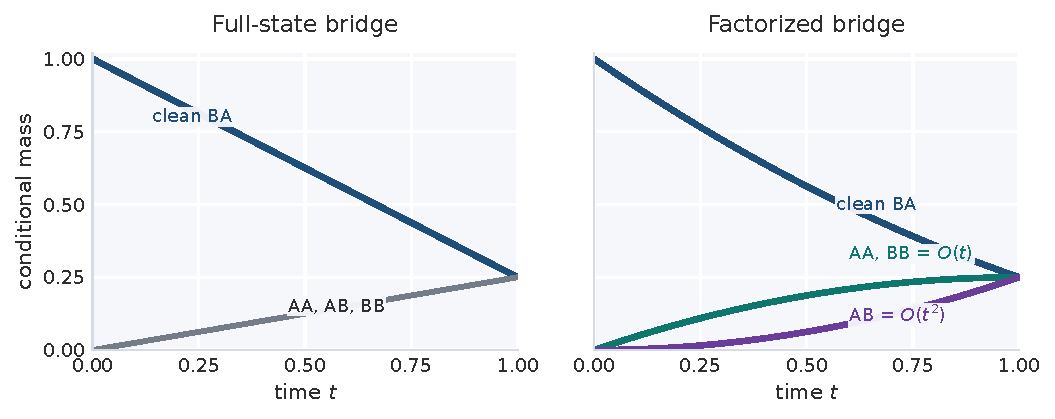
\includegraphics[width=0.92\textwidth]{figures/handouts/discrete_diffusion/fig_discrete_bridge_probabilities}
  \caption{Condition on the current bridge state \texttt{BA} in a two-token binary example.
  Under the exact full-state bridge, the alternative endpoint sequences \texttt{AA}, \texttt{AB}, and \texttt{BB} all enter at first order because one bridge time controls the whole sequence.
  Under the factorized bridge, \texttt{AA} and \texttt{BB} require one backward switch, while \texttt{AB} requires two independent switches and therefore appears only at second order.}
  \label{fig:full-vs-factorized-probabilities}
\end{figure}

This two-token toy calculation is the cleanest reason that coordinatewise marginals become sufficient after factorization.
The same distinction becomes more geometric on the two-dimensional ring example from the diffusion-models unit once we discretize the plane to a grid.
Bin the ring-mixture data law onto that grid, discretize the Gaussian reference law coordinatewise, and apply the factorized bridge \eqref{eq:factorized-mixture-path}.
At the level of marginals we still see the same kind of interpolation from the data endpoint law to the reference endpoint law.
The difference is in the sample-path geometry: the bridge no longer traces a Euclidean curve, and it instead moves by coordinatewise jumps between grid cells.

\begin{figure}[t]
  \centering
  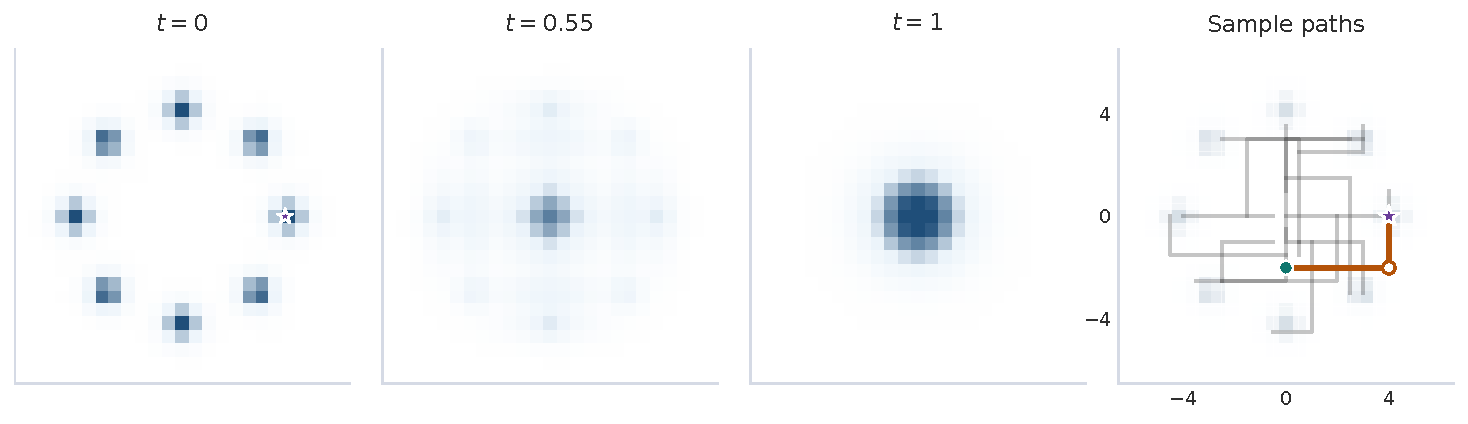
\includegraphics[width=\textwidth]{figures/handouts/discrete_diffusion/fig_discrete_spatial_bridge}
  \caption{A discretized version of the two-dimensional ring-mixture bridge.
  The first three panels show the bridge marginals on the grid at \(t=0\), \(t=0.55\), and \(t=1\).
  The last panel shows sample paths of the factorized bridge; the highlighted path starts from the starred data cell and ends at the teal reference draw.
  The marginal bridge still interpolates between the same endpoint laws, but individual paths move by one-coordinate jumps.}
  \label{fig:discrete-spatial-bridge}
\end{figure}

This is the discrete counterpart of the expectation-based picture in the continuous-state part of the diffusion-models unit.
There one learns a conditional expectation and reads off a velocity field on \(\R^2\).
Here the same bridge logic produces local jump intensities instead of a spatial vector field, which is why the finite-state description naturally passes through a generator.

For a sequence \(x\in\mathcal{V}^d\), let \(x^{j\to v}\) denote the neighbor obtained by replacing coordinate \(j\) by token \(v\).
The endpoint-conditioned generator is then as simple as possible.

\begin{proposition}[Endpoint-conditioned backward switch rule for the factorized bridge]
\label{prop:factorized-conditional-generator}
Let \(c_t\coloneqq -\dot\alpha_t/(1-\alpha_t)\), and assume \(0<\alpha_t<1\).
Then for every single-token neighbor \(x^{j\to v}\),
\begin{equation}
  Q_t^{x_0}\!\bigl(x^{j\to v}\mid x\bigr)
  =
  c_t\,\mathbf{1}\{v=x_{0,j}\}\,\mathbf{1}\{x_j\neq x_{0,j}\},
  \label{eq:factorized-conditional-generator}
\end{equation}
with diagonal chosen so that \(\sum_y Q_t^{x_0}(y\mid x)=0\).
\end{proposition}
\begin{proof}
Fix \(x_0\) and \(x\), and use the coordinatewise coupling \eqref{eq:factorized-coupling}.
If \(x_j=x_{0,j}\), then stepping backward does not require any change at coordinate \(j\).
If \(x_j\neq x_{0,j}\), conditioning on \(X_0=x_0\) and \(X_t=x\) forces \(\tau_j\le t\) and \(\Xi_j=x_j\), and the coordinate switches back exactly when \(\tau_j\in(t-h,t]\).
Therefore
\[
  \mathbb{P}(X_{t-h,j}=x_{0,j}\mid X_0=x_0,X_t=x, x_j\neq x_{0,j})
  =
  \frac{\alpha_{t-h}-\alpha_t}{1-\alpha_t}
  =
  hc_t+o(h).
\]
Independence of the switch times implies that simultaneous switches of two distinct coordinates are \(O(h^2)\), so they disappear at generator scale.
The only off-diagonal first-order moves are the backward switches in \eqref{eq:factorized-conditional-generator}.%
\end{proof}

To pass from the endpoint-conditioned generator to the marginal generator, we use the same posterior-averaging step as in the diffusion-models unit.

\begin{proposition}[Generator-level marginalization on a finite state space]
\label{prop:generator-marginalization}
Suppose
\[
  K_{t-h\mid t}(y\mid x)
  =
  \delta_x(y)+hQ_t(y\mid x)+o(h)
\]
and
\[
  K^{x_0}_{t-h\mid t}(y\mid x)
  =
  \delta_x(y)+hQ_t^{x_0}(y\mid x)+o(h)
\]
as \(h\downarrow 0\).
Then
\[
  Q_t(y\mid x)
  =
  \sum_{x_0\in S} Q_t^{x_0}(y\mid x)\,q_{0\mid t}(x_0\mid x).
\]
\end{proposition}
\begin{proof}
Apply \Cref{prop:finite-state-kernel-marginalization} with \(s=t-h\), insert the first-order expansions, subtract the common zeroth-order term \(\delta_x(y)\), divide by \(h\), and let \(h\downarrow 0\).%
\end{proof}

\begin{theorem}[Factorized generator rates depend only on coordinate marginals]
\label{thm:factorized-rates}
For the factorized mixture path \eqref{eq:factorized-mixture-path}, every off-diagonal single-token jump satisfies
\begin{equation}
  Q_t\!\bigl(x^{j\to v}\mid x\bigr)
  =
  c_t\,q_{0\mid t}\!\bigl(X_{0,j}=v\mid X_t=x\bigr),
  \qquad v\neq x_j.
  \label{eq:factorized-rate}
\end{equation}
\end{theorem}
\begin{proof}
Combine \Cref{prop:generator-marginalization} and \Cref{prop:factorized-conditional-generator}:
\[
  Q_t\!\bigl(x^{j\to v}\mid x\bigr)
  =
  \sum_{x_0\in S}
  c_t\,\mathbf{1}\{x_{0,j}=v\}\,\mathbf{1}\{x_j\neq x_{0,j}\}\,
  q_{0\mid t}(x_0\mid x).
\]
If \(v\neq x_j\), then the second indicator is automatically one on the event \(\{x_{0,j}=v\}\), so
\[
  Q_t\!\bigl(x^{j\to v}\mid x\bigr)
  =
  c_t\sum_{x_0\in S}\mathbf{1}\{x_{0,j}=v\}\,q_{0\mid t}(x_0\mid x)
  =
  c_t\,q_{0\mid t}(X_{0,j}=v\mid X_t=x).
\]
\end{proof}

If we write
\[
  \mu_{t,j}(x)\coloneqq \E[e_{X_{0,j}}\mid X_t=x]\in\R^{|\mathcal{V}|},
\]
then \Cref{thm:factorized-rates} becomes
\begin{equation}
  Q_t\!\bigl(x^{j\to v}\mid x\bigr)
  =
  c_t\,\mu_{t,j}(x)_v,
  \qquad v\neq x_j.
  \label{eq:factorized-rate-onehot}
\end{equation}
This is the cleanest statement of the simplification.
The full posterior over endpoint sequences has not disappeared.
It is still the exact posterior \(q_{0\mid t}(x_0\mid x)\) of the factorized bridge.
What the factorized bridge changes is the local move set: once only one-token backward switches are allowed at first order, the reverse rates query that posterior only through one-coordinate marginals.
So the approximation is in the bridge geometry, not in the posterior-averaging principle.
This is the generator-level reason that tokenwise classification becomes the practical training target.
The next theorem makes that precise: once the factorized bridge has been chosen, exact coordinate posteriors recover its exact reverse generator.

The full-state theorem above says that exact reverse kernels recover the correct law on any time grid.
For the factorized bridge, the parallel statement is now infinitesimal:
an ideal coordinatewise posterior model recovers the exact reverse generator of the chosen factorized bridge.
Recovering the corresponding marginal path on a time grid is then a separate numerical question, handled below by a bound in terms of accumulated one-step kernel error.

\begin{proposition}[Reverse Kolmogorov equation on a finite state space]
\label{prop:reverse-kolmogorov}
Let \(S\) be finite, let \(\pi_t\) be a differentiable path of probability mass functions on \(S\), and let \(Q_t\) be rate matrices whose entries depend continuously on \(t\).
Then the short-time relation
\[
  \pi_{t-h}(y)
  =
  \sum_{x\in S}
  \pi_t(x)\bigl[\delta_x(y)+hQ_t(y\mid x)\bigr]
  +o(h)
\]
for every \(y\in S\) is equivalent to the reverse Kolmogorov equation
\[
  -\frac{d}{dt}\pi_t(y)
  =
  \sum_{x\in S}
  \pi_t(x)\,Q_t(y\mid x),
  \qquad y\in S.
\]
Given the terminal condition \(\pi_1\), this linear ODE has a unique solution.
\end{proposition}
\begin{proof}
Because \(\sum_x \pi_t(x)\delta_x(y)=\pi_t(y)\), the short-time relation is
\[
  \pi_{t-h}(y)
  =
  \pi_t(y)
  +
  h\sum_{x\in S}\pi_t(x)\,Q_t(y\mid x)
  +
  o(h).
\]
Subtract \(\pi_t(y)\), divide by \(h\), and let \(h\downarrow 0\) to obtain the reverse Kolmogorov equation.
Conversely, if the reverse Kolmogorov equation holds, then differentiability gives
\[
  \pi_{t-h}(y)
  =
  \pi_t(y)-h\dot\pi_t(y)+o(h)
  =
  \pi_t(y)
  +
  h\sum_{x\in S}\pi_t(x)\,Q_t(y\mid x)
  +
  o(h),
\]
which is the short-time relation.
Uniqueness follows because this is a linear ODE on the finite-dimensional space \(\R^{|S|}\).%
\end{proof}

\begin{theorem}[Exact coordinate posteriors recover the factorized reverse generator]
\label{thm:factorized-infinitesimal-exactness}
For the factorized mixture path \eqref{eq:factorized-mixture-path}, suppose a model returns the exact coordinate marginals
\[
  \rho_{t,j}^\star(v\mid x)
  =
  q_{0\mid t}(X_{0,j}=v\mid X_t=x).
\]
Define the learned generator by
\[
  \hat Q_t^\star\!\bigl(x^{j\to v}\mid x\bigr)
  \coloneqq
  c_t\,\rho_{t,j}^\star(v\mid x),
  \qquad v\neq x_j,
\]
with diagonal chosen so that \(\sum_y \hat Q_t^\star(y\mid x)=0\).
Then \(\hat Q_t^\star=Q_t\), where \(Q_t\) is the exact reverse generator of the factorized bridge.
Consequently the factorized marginal path \(p_t\) is the unique solution of
\[
  -\frac{d}{dt}p_t(y)
  =
  \sum_{x\in S} p_t(x)\,\hat Q_t^\star(y\mid x),
  \qquad
  p_1 \text{ fixed},
\]
so the exact reverse CTMC for the factorized bridge transports the factorized marginal path back to \(p_0\).
\end{theorem}
\begin{proof}
The equality \(\hat Q_t^\star=Q_t\) is exactly \Cref{thm:factorized-rates}.
Because \(Q_t\) is the exact reverse generator of the factorized bridge,
\[
  K_{t-h\mid t}(y\mid x)
  =
  \delta_x(y)+hQ_t(y\mid x)+o(h).
\]
Combining this with \Cref{prop:reverse-kernels-transport} gives
\[
  p_{t-h}(y)
  =
  \sum_{x\in S}
  p_t(x)\bigl[\delta_x(y)+hQ_t(y\mid x)\bigr]
  +o(h).
\]
By \Cref{prop:reverse-kolmogorov}, the path \(p_t\) therefore solves the reverse Kolmogorov equation with generator \(Q_t=\hat Q_t^\star\).
Uniqueness gives the claim.%
\end{proof}

At this point the modeling approximation is fully visible.
The full-state sequence model and the factorized sequence model are different bridges, so they have different posteriors and different intermediate marginals.
But once the factorized bridge is chosen, \Cref{thm:factorized-infinitesimal-exactness} says that exact coordinate posteriors recover its exact reverse generator.
Equivalently, within the factorized model class the marginal dynamics are completely identified by the coordinate posteriors.
The remaining approximation is then only numerical: how accurately a discrete-time sampler tracks that reverse CTMC.

The exactness theorem above identifies the practical target immediately.
Inside the factorized bridge, learning the reverse dynamics means learning the coordinatewise posterior marginals that determine the reverse rates.
A network \(\rho_t^\theta\) therefore takes a current bridge state \(x\) and time \(t\) and outputs
\[
  \rho_{t,j}^\theta(v\mid x)
  \approx
  q_{0\mid t}(X_{0,j}=v\mid X_t=x).
\]
These outputs are still posterior objects: the full vector \(\mu_t(x)\) in the one-token case and the coordinatewise vectors \(\mu_{t,j}(x)\) in the factorized sequence case.
The statistical question is whether \(\rho_t^\theta\) learns the correct marginals.
The numerical question, which enters only after the model is trained, is how accurately a discrete-time sampler tracks the reverse CTMC determined by those marginals.
Tokenwise cross-entropy addresses the first question.

\begin{proposition}[Cross-entropy is the proper factorized objective]
\label{prop:cross-entropy-proper}
Fix \(t,x,j\), and write
\[
  \pi_j(v)\coloneqq q_{0\mid t}(X_{0,j}=v\mid X_t=x).
\]
For any candidate categorical distribution \(\rho(v)\),
\[
  \E_{V\sim \pi_j}[-\log \rho(V)]
  =
  H(\pi_j)+\operatorname{KL}(\pi_j\|\rho).
\]
Hence the expected tokenwise negative log-likelihood is minimized uniquely at \(\rho=\pi_j\).
\end{proposition}
\begin{proof}
Expand the expectation and add/subtract \(\log \pi_j(v)\):
\[
  \E_{V\sim \pi_j}[-\log \rho(V)]
  =
  \sum_v \pi_j(v)\log\frac{\pi_j(v)}{\rho(v)}
  -
  \sum_v \pi_j(v)\log \pi_j(v)
  =
  \operatorname{KL}(\pi_j\|\rho)+H(\pi_j).
\]
Only the KL term depends on \(\rho\), and it is minimized uniquely when \(\rho=\pi_j\).%
\end{proof}

The corresponding training loss is
\begin{equation}
  \mathcal{L}_{\mathrm{disc}}(\theta)
  =
  \E_{X_0\sim p_0,\; X_t\sim K_{t\mid 0}(\cdot\mid X_0),\; t\sim \mathrm{Unif}[0,1]}
  \left[
    \sum_{j=1}^d
    -\log \rho_{t,j}^\theta(X_{0,j}\mid X_t)
  \right],
  \label{eq:discrete-classification-loss}
\end{equation}
which is exactly the discrete flow-matching objective used by \citet[Eq.~(28) and Prop.~5]{gat2024discrete}.
So classification is not an extra heuristic layered on top of the bridge picture.
It is the proper scoring rule for the posterior statistics that the factorized generator actually needs.
It therefore gives the training loop directly.

\begin{algorithm}[H]
  \caption{Training a factorized discrete diffusion model}
  \label{alg:discrete-diffusion-training}
  \begin{algorithmic}[1]
    \Require Data sampler for \(p_0\), base marginals \(r_1,\dots,r_d\), schedule \(\alpha_t\), posterior network \(\rho_t^\theta\)
    \For{training steps}
      \State Sample \(x_0\sim p_0\) and \(t\sim \mathrm{Unif}[0,1]\)
      \For{\(j=1,\dots,d\) in parallel}
        \State Sample \(B_j\sim \mathrm{Bernoulli}(\alpha_t)\) and \(\Xi_j\sim r_j\)
        \If{\(B_j=1\)}
          \State Set \(x_{t,j}\gets x_{0,j}\)
        \Else
          \State Set \(x_{t,j}\gets \Xi_j\)
        \EndIf
      \EndFor
      \State Form \(x_t=(x_{t,1},\dots,x_{t,d})\)
      \State Evaluate \(\rho_{t,j}^\theta(\cdot\mid x_t)\) for all \(j\)
      \State Compute \(\ell\gets \sum_{j=1}^d -\log \rho_{t,j}^\theta(x_{0,j}\mid x_t)\)
      \State Take a gradient step on \(\ell\)
    \EndFor
  \end{algorithmic}
\end{algorithm}

Once \(\rho_t^\theta\) is trained, we obtain an approximate generator by
\[
  \hat Q_t^\theta(x^{j\to v}\mid x)
  =
  c_t\,\rho_{t,j}^\theta(v\mid x),
  \qquad v\neq x_j.
\]
An exact simulator would sample a CTMC from this generator.
For intuition, the simplest approximation is a parallel Euler step, which keeps the \(O(h)\) single-token events and ignores the \(O(h^2)\) simultaneous jumps over a step of size \(h\).

\begin{algorithm}[H]
  \caption{Euler sampling for the learned CTMC}
  \label{alg:discrete-diffusion-sampling}
  \begin{algorithmic}[1]
    \Require Base sampler for \(p_1\), time grid \(1=t_K>\cdots>t_0=0\), schedule factor \(c_t\), learned posterior network \(\rho_t^\theta\)
    \State Sample \(X_{t_K}\sim p_1\)
    \For{\(k=K,K-1,\dots,1\)}
      \State Set \(t\gets t_k\), \(h\gets t_k-t_{k-1}\), \(x\gets X_{t_k}\)
      \State Evaluate \(\rho_{t,j}^\theta(\cdot\mid x)\) for all coordinates \(j\)
      \For{\(j=1,\dots,d\) in parallel}
        \For{each \(v\neq x_j\)}
          \State \(\tilde p_j(v\mid x_j)\gets h\,c_t\,\rho_{t,j}^\theta(v\mid x)\)
        \EndFor
        \State \(\tilde p_j(x_j\mid x_j)\gets 1-h\sum_{v\neq x_j} c_t\,\rho_{t,j}^\theta(v\mid x)\)
        \State Sample \(X_{t_{k-1},j}\sim \mathrm{Categorical}(\tilde p_j(\cdot\mid x_j))\)
      \EndFor
      \State Set \(X_{t_{k-1}}\gets (X_{t_{k-1},1},\dots,X_{t_{k-1},d})\)
    \EndFor
    \State \Return \(X_{t_0}\)
  \end{algorithmic}
\end{algorithm}

Euler is only the time discretization.
The structural approximation happened earlier, when we replaced the full \(|\mathcal{V}|^d\)-state model by the factorized local bridge.
That distinction matters because classification is learning the posterior statistics needed by the chosen local generator, while Euler is only approximating the CTMC generated by those statistics.
For the per-coordinate categorical probabilities in \Cref{alg:discrete-diffusion-sampling} to be valid, we choose a grid fine enough that
\[
  h\,c_t\le 1
\]
at every step; this guarantees \(\tilde p_j(x_j\mid x_j)\ge 0\).
With that understood, the Euler sampler is one concrete family of approximate kernels \(\hat K_k\).

This isolates the remaining numerical question.
Fix a time grid and let \(K_k=K_{t_{k-1}\mid t_k}\) denote the exact reverse kernels of the factorized bridge on that grid.
Any practical sampler, including \Cref{alg:discrete-diffusion-sampling}, replaces \(K_k\) by approximate kernels \(\hat K_k\).
The only question is how those one-step kernel errors accumulate.

\begin{proposition}[Accumulated one-step kernel error controls gridwise marginal error]
\label{prop:accumulated-kernel-error}
Fix a decreasing grid \(1=t_K>\cdots>t_0=0\).
Let \(K_k=K_{t_{k-1}\mid t_k}\) be the exact reverse kernels of a bridge path, and let \(\hat K_k\) be any approximate reverse kernels on the same grid.
Start both chains from the same terminal law,
\[
  p_K=\hat p_K=p_1,
\]
and define
\[
  p_{k-1}=p_k K_k,
  \qquad
  \hat p_{k-1}=\hat p_k \hat K_k,
  \qquad k=K,\dots,1.
\]
For each step set
\[
  \varepsilon_k
  \coloneqq
  \sup_{x\in S}
  \sum_{y\in S}
  \bigl|\hat K_k(y\mid x)-K_k(y\mid x)\bigr|.
\]
Then for every \(m=0,\dots,K\),
\[
  \|\hat p_m-p_m\|_1
  \le
  \sum_{k=m+1}^K \varepsilon_k.
\]
In particular,
\[
  \|\hat p_0-p_0\|_1
  \le
  \sum_{k=1}^K \varepsilon_k.
\]
\end{proposition}
\begin{proof}
If \(m\) is any signed mass function on \(S\) and \(K\) is any Markov kernel, then
\[
  \|mK\|_1
  =
  \sum_{y\in S}
  \left|\sum_{x\in S} m(x)\,K(y\mid x)\right|
  \le
  \sum_{x\in S}|m(x)|\sum_{y\in S}K(y\mid x)
  =
  \|m\|_1.
\]
So Markov kernels are \(\ell_1\)-contractive.
Now
\[
  \hat p_{k-1}-p_{k-1}
  =
  (\hat p_k-p_k)\hat K_k
  +
  p_k(\hat K_k-K_k),
\]
and therefore
\[
  \|\hat p_{k-1}-p_{k-1}\|_1
  \le
  \|(\hat p_k-p_k)\hat K_k\|_1
  +
  \|p_k(\hat K_k-K_k)\|_1
  \le
  \|\hat p_k-p_k\|_1+\varepsilon_k.
\]
Iterating backward from \(\|\hat p_K-p_K\|_1=0\) gives the stated bound for every grid point.%
\end{proof}

\begin{corollary}[Small-step recovery of the factorized marginal path]
\label{cor:factorized-small-step-recovery}
Consider the factorized bridge \eqref{eq:factorized-mixture-path}, and suppose the learned posterior model is ideal so that \(\rho_{t,j}^\star(v\mid x)=q_{0\mid t}(X_{0,j}=v\mid X_t=x)\).
For each grid \(\Pi^{(n)}=\{1=t^{(n)}_{K_n}>\cdots>t^{(n)}_0=0\}\), let \(K_k^{(n)}\) be the exact reverse kernels of the factorized bridge and let \(\hat K_k^{(n)}\) be any approximate kernels built from those exact coordinate marginals.
If
\[
  \sum_{k=1}^{K_n}
  \sup_{x\in S}\sum_{y\in S}
  \bigl|\hat K_k^{(n)}(y\mid x)-K_k^{(n)}(y\mid x)\bigr|
  \longrightarrow 0
  \qquad\text{as } n\to\infty,
\]
then the approximate reverse chain converges at every grid point to the marginal path of the factorized bridge.
In particular,
\[
  \|\hat p_0^{(n)}-p_0\|_1\to 0.
\]
\end{corollary}
\begin{proof}
By \Cref{thm:factorized-infinitesimal-exactness}, the exact coordinate marginals recover the exact reverse generator of the factorized bridge.
Hence the exact reverse kernels \(K_k^{(n)}\) are the correct kernels for that bridge on the grid \(\Pi^{(n)}\).
Applying \Cref{prop:accumulated-kernel-error} to each grid gives the result.%
\end{proof}

This is the precise sense in which the practical factorized sampler becomes exact.
It does not say that the factorized bridge reproduces the exact full-state bridge on \(\mathcal{V}^d\); that modeling approximation was made earlier.
It says that once the factorized bridge is chosen, exact coordinate posteriors plus vanishing one-step kernel error recover its marginal path, and therefore its data endpoint \(p_0\), in the many-step limit.

\begin{exercise}[Reading factorized reverse rates]
\label{ex:reading-factorized-rates}
Stay inside the factorized bridge on the binary vocabulary \(\mathcal{V}=\{A,B\}\), and let the current bridge state be \(x=\texttt{BA}\).
Suppose
\[
  q_{0\mid t}(X_{0,1}=A\mid X_t=x)=0.6,
  \qquad
  q_{0\mid t}(X_{0,1}=B\mid X_t=x)=0.4,
\]
\[
  q_{0\mid t}(X_{0,2}=A\mid X_t=x)=0.2,
  \qquad
  q_{0\mid t}(X_{0,2}=B\mid X_t=x)=0.8,
\]
and \(c_t=3\).
\begin{enumerate}[leftmargin=*]
  \item Compute the off-diagonal reverse rates from \(\texttt{BA}\) to \(\texttt{AA}\) and to \(\texttt{BB}\).
  \item Compute the diagonal entry \(Q_t(\texttt{BA}\mid \texttt{BA})\).
  \item Explain why no table of joint probabilities \(q_{0\mid t}(X_{0,1},X_{0,2}\mid X_t=x)\) appears in these rates.
\end{enumerate}
\end{exercise}
\SolutionBox[10]{The neighbor \(\texttt{AA}\) is \(x^{1\to A}\), so \eqref{eq:factorized-rate} gives
\[
  Q_t(\texttt{AA}\mid \texttt{BA})
  =
  3\cdot q_{0\mid t}(X_{0,1}=A\mid X_t=x)
  =
  3(0.6)
  =
  1.8.
\]
Similarly \(\texttt{BB}=x^{2\to B}\), so
\[
  Q_t(\texttt{BB}\mid \texttt{BA})
  =
  3\cdot q_{0\mid t}(X_{0,2}=B\mid X_t=x)
  =
  3(0.8)
  =
  2.4.
\]
The row sum must vanish, hence
\[
  Q_t(\texttt{BA}\mid \texttt{BA})=-(1.8+2.4)=-4.2.
\]
No joint two-token table appears because the factorized bridge only allows one-token backward switches at first order.
Once the local move set is restricted to \(x^{j\to v}\), the reverse generator queries the posterior only through one-coordinate marginals.}

\begin{exercise}[Why only one-token jumps survive at first order]
\label{ex:one-token-jumps}
Use the factorized coupling \eqref{eq:factorized-coupling}.
Fix two distinct coordinates \(j\neq k\), and suppose both are currently away from their \(t=0\) endpoint values, so \(x_j\neq x_{0,j}\) and \(x_k\neq x_{0,k}\).
\begin{enumerate}[leftmargin=*]
  \item Show that
  \[
    \mathbb{P}\bigl(X_{t-h,j}=x_{0,j},\,X_{t-h,k}=x_{0,k}\mid X_0=x_0,\;X_t=x\bigr)
    =
    O(h^2).
  \]
  \item Explain why this implies that two-token jumps disappear at generator scale.
  \item Conclude that the generator-level reverse object only needs the coordinate marginals \(q_{0\mid t}(X_{0,j}=v\mid X_t=x)\), not simultaneous two-token switch probabilities.
\end{enumerate}
\end{exercise}
\SolutionBox[12]{Conditionally on \(X_0=x_0\) and \(X_t=x\), each coordinate that is away from its \(t=0\) endpoint switches back exactly when its switch time lies in \((t-h,t]\).
For one coordinate this has probability
\[
  \mathbb{P}(\tau_j\in (t-h,t]\mid \tau_j\le t)
  =
  hc_t+o(h).
\]
Because the switch times are independent across coordinates,
\begin{align*}
  &\mathbb{P}\bigl(X_{t-h,j}=x_{0,j},\,X_{t-h,k}=x_{0,k}\mid X_0=x_0,\;X_t=x\bigr) \\
  &\qquad=
  \mathbb{P}(\tau_j\in (t-h,t]\mid \tau_j\le t)\,
  \mathbb{P}(\tau_k\in (t-h,t]\mid \tau_k\le t)
  =
  \bigl(hc_t+o(h)\bigr)^2
  =
  O(h^2).
\end{align*}
After dividing by \(h\) to form the generator, any \(O(h^2)\) event vanishes.
So the first-order reverse dynamics can only move along one-token neighbors.
That is the structural reason the generator depends only on one-coordinate posterior marginals: simultaneous two-token switch probabilities never appear at first order.}

\subsection{Masked diffusion as a sharpened special case}
\label{subsec:masked-diffusion}

Masked diffusion makes the factorized story even cleaner by collapsing the reference law to a point mass.
It is not a new approximation layer; it is a particularly simple factorized bridge.
Adjoin an absorbing token \([\mathrm{MASK}]\notin\mathcal{V}\), set \(r_j=\delta_{[\mathrm{MASK}]}\) for every coordinate, and let
\[
  p_1=\delta_{[\mathrm{MASK}]^d}.
\]
Each coordinate now either keeps the \(t=0\) endpoint token or is replaced by \([\mathrm{MASK}]\).
Equivalently, the factorized bridge becomes
\begin{equation}
  K_{t\mid 0}(x\mid x_0)
  =
  \prod_{j=1}^d
  \Bigl[
    \alpha_t\,\delta_{x_{0,j}}(x_j)
    +
    (1-\alpha_t)\,\delta_{[\mathrm{MASK}]}(x_j)
  \Bigr].
  \label{eq:masked-factorized-bridge}
\end{equation}
This is the absorbing-mask version of the same factorized bridge picture.

\begin{corollary}[Revealed coordinates are already solved]
\label{cor:masked-revealed}
If \(X_{t,j}\neq [\mathrm{MASK}]\), then
\[
  q_{0\mid t}(X_{0,j}=X_{t,j}\mid X_t)=1
\]
and
\[
  q_{0\mid t}(X_{0,j}=v\mid X_t)=0
  \qquad \text{for } v\neq X_{t,j}.
\]
\end{corollary}
\begin{proof}
Under the masked bridge, a revealed token can only arise by keeping the \(t=0\) endpoint token.
So any endpoint sequence compatible with \(X_t\) must satisfy \(X_{0,j}=X_{t,j}\).%
\end{proof}

The second simplification is specific to the absorbing mask.
Once the current state tells us which coordinates are revealed and which are masked, the schedule factor contributes the same scalar weight to every compatible endpoint sequence.
After normalization it cancels.

\begin{proposition}[The masked posterior does not depend on time]
\label{prop:masked-time-independent}
Let \(x\in(\mathcal{V}\cup\{[\mathrm{MASK}]\})^d\), and define
\[
  U(x)\coloneqq \{j:x_j\neq [\mathrm{MASK}]\},
  \qquad
  M(x)\coloneqq \{j:x_j=[\mathrm{MASK}]\}.
\]
For the masked factorized bridge,
\begin{equation}
  K_{t\mid 0}(x\mid x_0)
  =
  \alpha_t^{|U(x)|}(1-\alpha_t)^{|M(x)|}
  \prod_{j\in U(x)} \mathbf{1}\{x_{0,j}=x_j\}.
  \label{eq:masked-likelihood-factor}
\end{equation}
Consequently,
\begin{equation}
  q_{0\mid t}(x_0\mid x)
  \propto
  p_0(x_0)\prod_{j\in U(x)}\mathbf{1}\{x_{0,j}=x_j\},
  \label{eq:masked-posterior-t-free}
\end{equation}
so the posterior depends on the masked pattern and the revealed tokens, but not on \(t\).
\end{proposition}
\begin{proof}
Each revealed coordinate contributes \(\alpha_t\,\mathbf{1}\{x_{0,j}=x_j\}\), and each masked coordinate contributes \(1-\alpha_t\).
Multiplying over coordinates gives \eqref{eq:masked-likelihood-factor}.
Bayes' rule then yields
\[
  q_{0\mid t}(x_0\mid x)
  \propto
  p_0(x_0)\,\alpha_t^{|U(x)|}(1-\alpha_t)^{|M(x)|}
  \prod_{j\in U(x)}\mathbf{1}\{x_{0,j}=x_j\}.
\]
The schedule factor does not depend on \(x_0\), so it cancels during normalization.%
\end{proof}

Equivalently, once we observe a masked row \(x\), the posterior is just the data law \(p_0\) renormalized on the set of endpoint sequences that agree with the revealed coordinates \(x_{U(x)}\).
The only role of the forward schedule is to contribute the common scalar \(\alpha_t^{|U(x)|}(1-\alpha_t)^{|M(x)|}\), and that scalar disappears when we normalize.

This is the posterior explanation for two familiar implementation choices.
First, the network can ignore time in the purely masked setting because the target posterior is time-independent \citep[Prop.~6 and App.~E.8]{gat2024discrete}.
Second, the loss can be restricted to masked positions because revealed coordinates already have degenerate posteriors.
That is exactly why the absorbing mask collapses the generic bridge problem to ordinary prediction on the masked coordinates.

\begin{exercise}[Why the schedule cancels in the masked case]
\label{ex:masked-cancel}
Fix a masked bridge state \(x\), and let \(U(x)\) and \(M(x)\) denote its revealed and masked coordinates.
\begin{enumerate}[leftmargin=*]
  \item Starting from \eqref{eq:masked-likelihood-factor}, show that every endpoint sequence compatible with the revealed coordinates receives the same factor
  \[
    \alpha_t^{|U(x)|}(1-\alpha_t)^{|M(x)|}.
  \]
  \item Use Bayes' rule to derive \eqref{eq:masked-posterior-t-free}.
  \item For a masked coordinate \(j\in M(x)\), prove that for every token \(v\in\mathcal{V}\),
  \[
    q_{0\mid t}(X_{0,j}=v\mid X_t=x)
    =
    \mathbb{P}_{X_0\sim p_0}\bigl(X_{0,j}=v \mid X_{0,U(x)}=x_{U(x)}\bigr).
  \]
  \item Why can the loss be restricted to masked positions?
\end{enumerate}
\end{exercise}
\SolutionBox[14]{By \eqref{eq:masked-likelihood-factor},
\[
  K_{t\mid 0}(x\mid x_0)
  =
  \alpha_t^{|U(x)|}(1-\alpha_t)^{|M(x)|}
  \prod_{i\in U(x)}\mathbf{1}\{x_{0,i}=x_i\}.
\]
So every endpoint sequence \(x_0\) compatible with the revealed coordinates gets the same schedule-dependent factor, and every incompatible sequence gets likelihood zero.
Bayes' rule gives
\[
  q_{0\mid t}(x_0\mid x)
  \propto
  p_0(x_0)\,
  \alpha_t^{|U(x)|}(1-\alpha_t)^{|M(x)|}
  \prod_{i\in U(x)}\mathbf{1}\{x_{0,i}=x_i\}.
\]
The schedule factor does not depend on \(x_0\), so it cancels during normalization:
\[
  q_{0\mid t}(x_0\mid x)
  \propto
  p_0(x_0)\prod_{i\in U(x)}\mathbf{1}\{x_{0,i}=x_i\}.
\]
Therefore, for \(j\in M(x)\),
\[
  q_{0\mid t}(X_{0,j}=v\mid X_t=x)
  =
  \mathbb{P}_{X_0\sim p_0}\bigl(X_{0,j}=v \mid X_{0,U(x)}=x_{U(x)}\bigr).
\]
Revealed positions can be dropped from the loss because their posteriors are already point masses by \Cref{cor:masked-revealed}; only the masked coordinates still carry uncertainty.}

\subsection{Connection back to the Euclidean expectation lens}
\label{subsec:euclidean-connection}

The bridge-first parallel with the Euclidean setting can be written explicitly:
\[
  \begin{aligned}
    \text{Euclidean bridge:}\qquad
    &\text{learn }
    \E[\dot X_t\mid X_t=x]
    \text{ or }
    \E[X_0\mid X_t=x].\\[0.35em]
    \text{Full finite-state bridge on }S:\qquad
    &\text{learn }
    \E[e_{X_0}\mid X_t=x]
    =
    q_{0\mid t}(\cdot\mid x).\\[0.35em]
    \text{Factorized bridge on }\mathcal{V}^d:\qquad
    &\text{learn }
    \E[e_{X_{0,j}}\mid X_t=x]
    =
    q_{0\mid t}(X_{0,j}=\cdot\mid X_t=x)
    \text{ for each }j.
  \end{aligned}
\]

The Euclidean model cannot represent the full posterior by a finite-dimensional simplex vector, so it learns the conditional expectations under that posterior that are infinitesimally sufficient for the marginal dynamics.
The one-token discrete model can represent the full posterior exactly, because a one-hot expectation on a finite set is already a probability vector.
The factorized sequence model makes the parallel tractability move: it keeps the posterior-averaging principle but chooses a local jump geometry whose infinitesimal rates depend only on coordinatewise posterior marginals.
Within that factorized model, those marginals still recover the correct reverse dynamics and therefore the correct endpoint law \(p_0\).
That is the precise sense in which practical discrete diffusion reduces to classification.

So the clean conclusion is not that discrete diffusion secretly stops being distributional.
It is the opposite.
The exact finite-state story is fully distributional from the start, and tokenwise classification appears only after we decide to approximate the full sequence model by a factorized local bridge.

\begin{exercise}[Classify the bridge]
\label{ex:classify-the-bridge}
For each scenario below, decide whether the tokenwise-classification reduction developed above is exact at the generator level, exact only in the masked/time-independent special case, or only approximate.
In each case, identify the first-order reverse move set and the first model change you would try if that reduction fails.
\begin{enumerate}[leftmargin=*]
  \item A one-token categorical bridge with a known schedule.
  \item A factorized sequence bridge with independent switch times.
  \item A masked bridge where the network is trained only on masked positions.
  \item A coupled bridge in which two-token moves occur at first order.
\end{enumerate}
\end{exercise}
\SolutionBox[14]{For the one-token categorical bridge, classification is exact at the generator level:
the reverse chain can jump from the current token \(x\) to any token \(v\neq x\), and the rates are exactly the posterior coordinates \(q_{0\mid t}(X_0=v\mid X_t=x)\).
For the factorized sequence bridge, classification is again exact at the generator level:
the first-order move set consists of one-token neighbors \(x^{j\to v}\), and the corresponding rates are exactly the coordinate marginals \(q_{0\mid t}(X_{0,j}=v\mid X_t=x)\).
For the masked bridge, this is the masked/time-independent special case of the factorized bridge, so the reduction remains exact at the generator level:
the uncertain moves live only on masked coordinates, the posterior ignores \(t\), and training can therefore be restricted to masked positions whose posteriors are not already degenerate.
For a coupled bridge with two-token moves at first order, classification is only approximate.
The reverse generator now needs block moves or other nonlocal jumps, so a tokenwise classifier is missing the first-order object itself.
The first fix is to enlarge the learned reverse object, for example by modeling blockwise posteriors or a richer reverse kernel that can score coupled edits.}

\subsection{Other discrete variants}
\label{subsec:other-discrete-variants}

The discussion above focused on one model class:
a factorized bridge, its reverse CTMC, and the discrete flow-matching objective that learns the posterior marginals needed by that generator.
That is the cleanest setup for developing the distributional picture without fragmentation.

Other named discrete diffusion models can mostly be understood as changing one of three ingredients while keeping the same bridge-first logic.
The uniform multinomial kernel of \citet[\S4]{hoogeboom2021argmax} is the basic one-token categorical instance of this story.
Absorbing-mask models are the sharpened special case from \Cref{subsec:masked-diffusion}; in discrete time this is the absorbing-state construction in \citet[\S3.1]{austin2021structured}, while in the present flow-matching setup the posterior simplification is exactly the one stated in \citep[Prop.~6 and App.~E.8]{gat2024discrete}.
Richer D3PM-style constructions play the same role by changing the one-token forward corruption kernel in the discrete-time model \citep[\S3.1--3.3]{austin2021structured}; in the bridge-first view used here, that changes the local geometry while leaving the posterior-averaging principle intact.

So the real conceptual distinction is not between many separate algorithms.
It is between the exact full-state bridge, the tractable factorized bridge, and the numerical schemes used to approximate reverse-time sampling once that bridge has been chosen.
Carried back to the main notes, the lesson is the same as in the Euclidean diffusion story: choose a bridge, identify the conditional object that is sufficient for reverse-time transport, and then ask which tractable approximation preserves that sufficiency.
The discrete setting is simply the case where, for some bridges, that conditional object is a literal posterior vector rather than a lower-dimensional summary.

\bibliographystyle{plainnat}
\makeatletter
\begingroup
\let\input@path\@empty
\IfFileExists{references.bib}{%
  \gdef\stat221bibpath{references}%
}{%
  \IfFileExists{../references.bib}{%
    \gdef\stat221bibpath{../references}%
  }{%
    \gdef\stat221bibpath{../../references}%
  }%
}
\endgroup
\makeatother
\bibliography{\stat221bibpath}

\end{document}
"
%   (Low-level direct build: if you invoke latexmk manually, set -jobname to the
%    titled output so the compiled PDF matches the standard naming scheme.)
\newif\ifshowsolutions
\showsolutionsfalse
\ifdefined\STATshowsolutions
  \showsolutionstrue
\fi
\ifcsname STAT221SOLUTIONS\endcsname
  \showsolutionstrue
\fi

% Solutions/workspace boxes (controlled by \ifshowsolutions).
% Usage: \SolutionBox[<workspace lines>]{<solution body>}
\newcommand{\SolutionBox}[2][10]{%
  \ifshowsolutions
    \begin{tcolorbox}[stat221panelgray,title={Solution}]
    #2
    \end{tcolorbox}
  \else
    \begin{tcolorbox}[stat221panelgray,unbreakable,title={Workspace}]
    \vspace{#1\baselineskip}
    \end{tcolorbox}
  \fi
}

\title{Discrete diffusion as posterior learning}
\author{}
\date{}

\begin{document}
\maketitle

\section[Discrete diffusion as posterior learning]{Discrete diffusion as posterior learning}
\label{sec:discrete-posterior-learning}

Fix a finite state space \(S\).
This handout takes the diffusion unit's bridge-first viewpoint and specializes it to a setting where the reverse-time object can sometimes be represented exactly.
The central ingredients are the endpoint laws \(p_0\) and \(p_1\), the chosen bridge \(K_{t\mid 0}(\cdot\mid x_0)\), and the endpoint posterior \(q_{0\mid t}\) induced by that bridge.
In finite state spaces the resulting question becomes unusually clean: when does reverse sampling reduce to classification, and when does tractability require a change in the bridge itself?

Let \(p_0\) be the data law on \(S\), let \(p_1\) be a reference law, and let \(K_{t\mid 0}(\cdot\mid x_0)\) be a conditional probability path with
\[
  K_{0\mid 0}(\cdot\mid x_0)=\delta_{x_0},
  \qquad
  K_{1\mid 0}(\cdot\mid x_0)=p_1.
\]
Averaging over \(X_0\sim p_0\) gives the marginal law \(p_t\), and Bayes' rule gives the endpoint posterior
\[
  q_{0\mid t}(x_0\mid x)
  =
  \frac{p_0(x_0)K_{t\mid 0}(x\mid x_0)}{p_t(x)}.
\]
If we knew this posterior exactly, reverse sampling would be straightforward:
sample an endpoint from \(q_{0\mid t}(\cdot\mid x)\) and then take the bridge step conditioned on that endpoint.
This is the finite-state specialization of the posterior-averaging mechanism developed in the diffusion-models unit.

When \(S\) is small, the one-hot conditional expectation \(\E[e_{X_0}\mid X_t=x]\) is already the full posterior vector \(q_{0\mid t}(\cdot\mid x)\).
For a one-token vocabulary model that means classifier outputs can represent the exact reverse-time object.
For the full sequence state space \(S=\mathcal{V}^d\), the same statement remains true but becomes computationally useless because the simplex has size \(|\mathcal{V}|^d\).
Practical discrete diffusion therefore changes the bridge, not the posterior-averaging principle: it replaces the exact full-sequence bridge by a coordinatewise bridge whose reverse generator depends only on coordinatewise posterior marginals.
The discussion below follows that progression from the exact finite-state bridge to the exact full-sequence model and then to the factorized sequence bridge used in practice.

\subsection{Exact posterior learning on a finite state space}
\label{subsec:finite-state-full-posterior}

We now specialize the bridge and posterior notation of the diffusion-models unit to a finite state space \(S\).
Let \(p_0\) be the data law, \(p_1\) a reference law, and
\[
  K_{t\mid 0}(\cdot\mid x_0),
  \qquad
  K_{0\mid 0}(\cdot\mid x_0)=\delta_{x_0},
  \qquad
  K_{1\mid 0}(\cdot\mid x_0)=p_1
\]
is a conditional probability path.
The corresponding marginal path is
\[
  p_t(x)=\sum_{x_0\in S} p_0(x_0)\,K_{t\mid 0}(x\mid x_0),
\]
and Bayes' rule gives the posterior over the \(t=0\) endpoint states,
\[
  q_{0\mid t}(x_0\mid x)
  =
  \frac{p_0(x_0)K_{t\mid 0}(x\mid x_0)}{p_t(x)}.
\]
This formula is understood on the support of \(p_t\), that is, for states \(x\) with \(p_t(x)>0\).

In the Euclidean development of the diffusion-models unit, one passes from the full posterior to conditional expectations that are infinitesimally sufficient.
On a finite state space, a one-hot embedding of the \(t=0\) endpoint loses no information, so the same conditional expectation is the full posterior itself.
Suppressing the dependence on \(S\), write \(e_z\in\R^{|S|}\) for the basis vector indexed by \(z\in S\).

\begin{proposition}[The one-hot conditional expectation is the full posterior]
\label{prop:full-state-onehot}
Define
\[
  \mu_t(x)\coloneqq \E[e_{X_0}\mid X_t=x]\in\R^{|S|}.
\]
Then
\begin{equation}
  \mu_t(x)_z
  =
  q_{0\mid t}(X_0=z\mid X_t=x),
  \qquad z\in S.
  \label{eq:full-state-onehot}
\end{equation}
\end{proposition}
\begin{proof}
Because \(e_{X_0}=e_z\) on the event \(\{X_0=z\}\),
\[
  \mu_t(x)
  =
  \sum_{z\in S} e_z\,\mathbb{P}(X_0=z\mid X_t=x).
\]
Taking the \(z\)th coordinate gives \eqref{eq:full-state-onehot}.%
\end{proof}

\Cref{prop:full-state-onehot} is the finite-state version of the Euclidean expectation reduction, except that here the reduction is exact.
In Euclidean space, quantities like \(\E[\dot X_t\mid X_t=x]\) or \(\E[X_0\mid X_t=x]\) summarize a richer posterior.
For a finite state space, the one-hot expectation \(\E[e_{X_0}\mid X_t=x]\) already is the posterior.
When \(S=\mathcal{V}\), a classifier over the vocabulary is therefore an exact posterior model.

\begin{figure}[t]
  \centering
  \begin{tikzpicture}[font=\small]
  \tikzset{
    panel/.style={
      rounded corners=7pt,
      draw=stat221Gray!30,
      fill=stat221GrayLight,
      line width=0.85pt,
    },
    infobox/.style={
      rounded corners=5pt,
      draw=stat221Blue!55!black,
      fill=white,
      line width=0.85pt,
      inner sep=8pt,
      text width=4.6cm,
      align=left,
    },
    coordlabel/.style={
      font=\footnotesize,
      fill=white,
      inner sep=1.5pt,
      text=stat221Gray,
    },
  }

  \path[use as bounding box] (-0.1,-0.1) rectangle (13.9,5.25);
  \draw[panel] (0,0) rectangle (13.7,4.95);

  \node[font=\small\bfseries,text=stat221Gray] at (3.10,4.58)
    {The posterior lives in the simplex};
  \node[font=\small\bfseries,text=stat221Gray] at (10.28,4.58)
    {Its coordinates are the reverse rates};

  \coordinate (A) at (0.95,0.78);
  \coordinate (B) at (5.85,0.78);
  \coordinate (C) at (3.40,3.95);
  \coordinate (P) at (2.76,1.50);

  \fill[white] (A) -- (B) -- (C) -- cycle;
  \draw[stat221Gray!70,line width=1.05pt] (A) -- (B) -- (C) -- cycle;

  % Constant-coordinate lines through the posterior point.
  \draw[stat221Blue!70!black,densely dashed,line width=1.0pt]
    ($(A)!0.5!(B)$) -- ($(A)!0.5!(C)$);
  \draw[stat221Green!70!black,densely dashed,line width=1.0pt]
    ($(B)!0.3!(A)$) -- ($(B)!0.3!(C)$);
  \draw[stat221Purple!70!black,densely dashed,line width=1.0pt]
    ($(C)!0.2!(A)$) -- ($(C)!0.2!(B)$);

  \filldraw[fill=stat221BlueLight,draw=stat221Blue!70!black,line width=0.9pt] (A) circle (0.16);
  \filldraw[fill=stat221GreenLight,draw=stat221Green!70!black,line width=0.9pt] (B) circle (0.16);
  \filldraw[fill=stat221PurpleLight,draw=stat221Purple!70!black,line width=0.9pt] (C) circle (0.16);
  \node[font=\small\bfseries,text=stat221Blue!75!black] at ($(A)+(-0.38,-0.28)$) {\(A\)};
  \node[font=\small\bfseries,text=stat221Green!60!black] at ($(B)+(0.38,-0.28)$) {\(B\)};
  \node[font=\small\bfseries,text=stat221Purple!60!black] at ($(C)+(0.00,0.35)$) {\(C\)};

  \filldraw[fill=stat221Gray,draw=white,line width=0.9pt] (P) circle (0.12);
  \draw[stat221Gray!60,line width=0.8pt] (P) -- +(0.55,0.55);
  \node[font=\small,text=stat221Gray,align=left] at ($(P)+(0.68,0.68)$)
    {\(\mu_t(x)\)};
  \node[font=\scriptsize,text=stat221Gray,align=left] at ($(P)+(0.92,0.28)$)
    {\(=q_{0\mid t}(\cdot\mid x)\)};

  \node[coordlabel,text=stat221Blue!75!black] at (1.80,2.38) {\(A=0.5\)};
  \node[coordlabel,text=stat221Green!60!black] at (4.85,2.10) {\(B=0.3\)};
  \node[coordlabel,text=stat221Purple!60!black] at (2.35,1.02) {\(C=0.2\)};

  \node[infobox] (info) at (10.30,2.45) {%
    \(\displaystyle \mu_t(x)=(0.5,\,0.3,\,0.2)\)

    \vspace{0.45em}
    \textcolor{stat221Blue!75!black}{\(Q_t^{\mathrm{rev}}(A\mid x)=0.5\,c_t\)}

    \textcolor{stat221Green!60!black}{\(Q_t^{\mathrm{rev}}(B\mid x)=0.3\,c_t\)}

    \textcolor{stat221Purple!60!black}{\(Q_t^{\mathrm{rev}}(C\mid x)=0.2\,c_t\)}

    \vspace{0.55em}
    The reverse generator is \(c_t\) times these coordinates.};
\end{tikzpicture}

  \caption{In the one-token setting, the posterior is literally a point in the simplex over endpoint states.
  Learning that point is genuinely distributional, and the reverse generator just rescales its coordinates by the common jump rate \(c_t\).}
  \label{fig:one-token-distributional}
\end{figure}

This is the discrete analogue of the conditional-versus-marginal story in the diffusion-models unit.
We observe the current bridge state \(X_t=x\), infer the conditional law of the endpoint \(X_0\mid X_t=x\), and then use a sampled endpoint to take the reverse bridge step.
The only difference from the Euclidean case is that on a finite set the relevant posterior can sometimes be represented exactly by a finite vector.

Operationally, an exact finite-state bridge can therefore be sampled in two stages.
Given a current state \(x_t\) and an earlier time \(s<t\), first draw an endpoint and then draw from the bridge conditioned on that endpoint:
\[
  \tilde X_0\sim q_{0\mid t}(\cdot\mid x_t),
  \qquad
  X_s\sim K^{\tilde X_0}_{s\mid t}(\cdot\mid x_t).
\]
Marginalizing \(\tilde X_0\) recovers the exact earlier-time kernel \(K_{s\mid t}(\cdot\mid x_t)\).
So in the one-token case there is no approximation to explain away: infer the full conditional law of \(X_0\mid X_t=x_t\), sample an endpoint from it, and then take the exact bridge step conditioned on that sample.

\begin{proposition}[Endpoint-conditioned bridge marginalization on a finite state space]
\label{prop:finite-state-kernel-marginalization}
Let \(0\le s\le t\le 1\).
Write \(K^{x_0}_{s\mid t}(\cdot\mid x_t)\) for the bridge kernel from time \(t\) to the earlier time \(s\) conditioned on the endpoint \(X_0=x_0\).
Then
\[
  K_{s\mid t}(y\mid x_t)
  =
  \sum_{x_0\in S}
  K^{x_0}_{s\mid t}(y\mid x_t)\,
  q_{0\mid t}(x_0\mid x_t).
\]
\end{proposition}
\begin{proof}
For states \(x_t\) with \(p_t(x_t)>0\), the law of total probability gives
\[
  \mathbb{P}(X_s=y\mid X_t=x_t)
  =
  \sum_{x_0\in S}
  \mathbb{P}(X_s=y\mid X_0=x_0,X_t=x_t)\,
  \mathbb{P}(X_0=x_0\mid X_t=x_t).
\]
This is exactly the displayed identity.%
\end{proof}

\begin{proposition}[Exact reverse kernels transport the marginal path]
\label{prop:reverse-kernels-transport}
For every \(0\le s\le t\le 1\),
\[
  p_s(y)
  =
  \sum_{x\in S} p_t(x)\,K_{s\mid t}(y\mid x),
  \qquad y\in S.
\]
\end{proposition}
\begin{proof}
Again by the law of total probability,
\[
  p_s(y)
  =
  \sum_{x\in S}
  \mathbb{P}(X_t=x)\,\mathbb{P}(X_s=y\mid X_t=x)
  =
  \sum_{x\in S} p_t(x)\,K_{s\mid t}(y\mid x).
\]
\end{proof}

The diffusion-models unit combines these two identities into a domain-agnostic exactness theorem:
if at every grid time \(t_k\) we can sample \(\tilde X_0\sim\mathrm{Law}(X_0\mid X_{t_k}=x)\) from the exact endpoint posterior and then sample the reverse step from \(K^{\tilde X_0}_{t_{k-1}\mid t_k}(\cdot\mid x)\), then reverse sampling is exact on any grid.
On a finite state space the same statement applies verbatim.
So for the exact one-token or full-sequence model there is no approximation to explain away: once the full posterior is exact, every reverse step uses the exact bridge kernel.
The generator formulas below are the infinitesimal version of that general result.

To make that infinitesimal picture concrete, consider the finite-state mixture path
\begin{equation}
  K_{t\mid 0}(x\mid x_0)
  =
  \alpha_t\,\delta_{x_0}(x)+(1-\alpha_t)\,r(x),
  \qquad x,x_0\in S,
  \label{eq:full-state-mixture-path}
\end{equation}
where \(r\) is a reference law on \(S\), and \(\alpha:[0,1]\to[0,1]\) is differentiable and nonincreasing with \(\alpha_0=1\) and \(\alpha_1=0\).
This is the simplest categorical bridge on a one-token state space.
If we instead take \(S=\mathcal{V}^d\), then \eqref{eq:full-state-mixture-path} is a mathematically exact non-factorized sequence model: the state space is all endpoint sequences, and the learned output would be a posterior over complete sequences rather than over individual coordinates.

A useful coupling introduces a single switch time.
Draw \(\tau\) with survival function \(\mathbb{P}(\tau>t)=\alpha_t\), draw \(\Xi\sim r\) independently, and set
\begin{equation}
  X_t=
  \begin{cases}
    X_0, & t<\tau,\\
    \Xi, & t\ge \tau.
  \end{cases}
  \label{eq:full-state-mixture-coupling}
\end{equation}
Then \eqref{eq:full-state-mixture-coupling} realizes exactly the bridge \eqref{eq:full-state-mixture-path}.
To describe reverse-time motion infinitesimally, we use a time-dependent rate matrix \(Q_t\), meaning that over a short backward step of length \(h\),
\[
  K_{t-h\mid t}(y\mid x)
  =
  \delta_x(y)+hQ_t(y\mid x)+o(h).
\]
So the off-diagonal entries \(Q_t(y\mid x)\) are first-order jump intensities from \(x\) to \(y\).

\begin{proposition}[Full-state generator rates are posterior probabilities]
\label{prop:full-state-rates}
Let \(K_{t\mid 0}\) be the full-state mixture path \eqref{eq:full-state-mixture-path}, and define
\[
  c_t\coloneqq -\frac{\dot\alpha_t}{1-\alpha_t},
  \qquad 0<\alpha_t<1.
\]
Then for every \(y\neq x\),
\begin{equation}
  Q_t(y\mid x)
  =
  c_t\,q_{0\mid t}(X_0=y\mid X_t=x)
  =
  c_t\,\mu_t(x)_y.
  \label{eq:full-state-rate}
\end{equation}
\end{proposition}
\begin{proof}
Fix \(x_0\in S\) and use the coupling \eqref{eq:full-state-mixture-coupling}.
If \(x\neq x_0\), then conditioning on \(X_0=x_0\) and \(X_t=x\) forces \(\tau\le t\) and \(\Xi=x\).
Moving from \(t\) to \(t-h\), the chain switches from \(x\) back to \(x_0\) exactly when \(\tau\in(t-h,t]\), so
\[
  \mathbb{P}(X_{t-h}=x_0\mid X_0=x_0,X_t=x)
  =
  \frac{\alpha_{t-h}-\alpha_t}{1-\alpha_t}
  =
  hc_t+o(h).
\]
No other off-diagonal jump is possible, and if \(x=x_0\) there is no off-diagonal jump at all.
So the endpoint-conditioned generator is
\[
  Q_t^{x_0}(y\mid x)
  =
  c_t\,\mathbf{1}\{y=x_0\}\,\mathbf{1}\{x\neq x_0\}.
\]
Averaging against the posterior gives
\[
  Q_t(y\mid x)
  =
  \sum_{x_0\in S} Q_t^{x_0}(y\mid x)\,q_{0\mid t}(x_0\mid x)
  =
  c_t\,q_{0\mid t}(X_0=y\mid X_t=x)
\]
for \(y\neq x\).
The identity with \(\mu_t(x)\) follows from \Cref{prop:full-state-onehot}.%
\end{proof}

Equation \eqref{eq:full-state-rate} is the infinitesimal version of the exact two-stage bridge step above.
It says that one-dimensional discrete diffusion is already fully distributional.
There is no distinction between predicting a label distribution and predicting the full posterior over endpoint states because those are the same vector when \(S=\mathcal{V}\).
The same statement remains mathematically true for \(S=\mathcal{V}^d\), but now the classifier would need \(|\mathcal{V}|^d\) outputs and the local bridge could point toward arbitrary full sequences.
That is exact and usually intractable.

\begin{exercise}[Posterior vector or label?]
\label{ex:posterior-vector-vs-label}
Stay in the one-token bridge \(S=\mathcal{V}\), fix a current token \(x\), and write
\[
  \mu_t(x)=\E[e_{X_0}\mid X_t=x].
\]
\begin{enumerate}[leftmargin=*]
  \item Use \eqref{eq:full-state-onehot} to show that \(\mu_t(x)\) is a probability vector on \(\mathcal{V}\).
  \item Using \eqref{eq:full-state-rate}, write the off-diagonal reverse rates \(Q_t(v\mid x)\) for \(v\neq x\) directly in terms of \(\mu_t(x)\).
  \item Explain why keeping only the argmax token \(\arg\max_v \mu_t(x)_v\) is not enough to reconstruct the reverse generator.
\end{enumerate}
\end{exercise}
\SolutionBox[10]{From \eqref{eq:full-state-onehot},
\[
  \mu_t(x)_v=q_{0\mid t}(X_0=v\mid X_t=x)\ge 0
  \qquad\text{for every }v\in\mathcal{V},
\]
and therefore
\[
  \sum_{v\in\mathcal{V}}\mu_t(x)_v
  =
  \sum_{v\in\mathcal{V}} q_{0\mid t}(X_0=v\mid X_t=x)
  =
  1.
\]
So \(\mu_t(x)\) lies in the simplex.
Equation \eqref{eq:full-state-rate} gives
\[
  Q_t(v\mid x)=c_t\,\mu_t(x)_v,
  \qquad v\neq x.
\]
Thus every off-diagonal rate is one coordinate of the posterior vector.
Keeping only the argmax token loses the sizes of the nonmaximal coordinates and therefore loses the relative jump intensities toward the other destinations.
It also loses the total escape rate
\[
  \sum_{v\neq x} Q_t(v\mid x)=c_t\bigl(1-\mu_t(x)_x\bigr),
\]
so even the diagonal entry cannot be reconstructed from the argmax alone.}

\begin{exercise}[A tiny vocabulary posterior and reverse-rate computation]
\label{ex:tiny-vocab}
Let \(\mathcal{V}=\{A,B,C\}\), let
\[
  p_0(A)=\frac12,
  \qquad
  p_0(B)=\frac13,
  \qquad
  p_0(C)=\frac16,
\]
let the reference law be uniform \(r(A)=r(B)=r(C)=1/3\), and suppose \(\alpha_t=1/4\).
If we observe \(X_t=B\), then:
\begin{enumerate}[leftmargin=*]
  \item Compute \(K_{t\mid 0}(B\mid A)\), \(K_{t\mid 0}(B\mid B)\), and \(K_{t\mid 0}(B\mid C)\).
  \item Use Bayes' rule to compute the posterior vector
  \[
    q_{0\mid t}(\cdot\mid B).
  \]
  \item If \(c_t=2\), compute the off-diagonal reverse rates \(Q_t(A\mid B)\) and \(Q_t(C\mid B)\), and then determine the diagonal entry \(Q_t(B\mid B)\).
\end{enumerate}
\end{exercise}
\SolutionBox[14]{The one-token bridge is
\[
  K_{t\mid 0}(x\mid x_0)=\alpha_t\,\delta_{x_0}(x)+(1-\alpha_t)\,r(x).
\]
With \(\alpha_t=1/4\) and \(r(B)=1/3\),
\[
  K_{t\mid 0}(B\mid A)=\frac34\cdot \frac13=\frac14,
  \qquad
  K_{t\mid 0}(B\mid B)=\frac14+\frac34\cdot \frac13=\frac12,
  \qquad
  K_{t\mid 0}(B\mid C)=\frac14.
\]
The unnormalized posterior weights are therefore
\[
  p_0(A)K_{t\mid 0}(B\mid A)=\frac12\cdot\frac14=\frac18,
  \qquad
  p_0(B)K_{t\mid 0}(B\mid B)=\frac13\cdot\frac12=\frac16,
  \qquad
  p_0(C)K_{t\mid 0}(B\mid C)=\frac16\cdot\frac14=\frac1{24}.
\]
Their sum is
\[
  \frac18+\frac16+\frac1{24}=\frac13,
\]
so
\[
  q_{0\mid t}(A\mid B)=\frac{1/8}{1/3}=\frac38,
  \qquad
  q_{0\mid t}(B\mid B)=\frac{1/6}{1/3}=\frac12,
  \qquad
  q_{0\mid t}(C\mid B)=\frac{1/24}{1/3}=\frac18.
\]
Using \eqref{eq:full-state-rate} with \(c_t=2\),
\[
  Q_t(A\mid B)=2\cdot \frac38=\frac34,
  \qquad
  Q_t(C\mid B)=2\cdot \frac18=\frac14.
\]
The row sum must vanish, so
\[
  Q_t(B\mid B)=-\Bigl(Q_t(A\mid B)+Q_t(C\mid B)\Bigr)=-1.
\]}

\subsection{The factorized bridge on sequences}
\label{subsec:factorized-approximation}

Now take sequences \(x_0\in\mathcal{V}^d\).
The previous subsection already tells us what the exact sequence model would be.
We would simply keep the same finite-state construction and enlarge the state space itself to \(S=\mathcal{V}^d\).
Then the posterior \(q_{0\mid t}(\cdot\mid x)\) would be a distribution over complete endpoint sequences, not over individual coordinates.
Nothing about posterior averaging changes in that exact model; the only change is that the simplex now has dimension \(|\mathcal{V}|^d-1\), which is conceptually clean and usually computationally hopeless.

Practical discrete diffusion therefore makes its tractability move at the level of the bridge, not at the level of posterior averaging.
Write \(K^{\mathrm{full}}_{t\mid 0}\), \(p_t^{\mathrm{full}}\), and \(q^{\mathrm{full}}_{0\mid t}\) for the exact full-state bridge, its marginal path, and its posterior.
We then replace that bridge by a coordinatewise bridge \(K^{\mathrm{fac}}_{t\mid 0}\), with its own marginal path \(p_t^{\mathrm{fac}}\) and posterior \(q^{\mathrm{fac}}_{0\mid t}\).
This is the modeling approximation.
The exact and factorized sequence models share the same endpoints \(p_0\) and \(p_1\), but for \(t\in(0,1)\) they induce different intermediate marginals and different posteriors because they are genuinely different bridges.
What survives unchanged is the organizing principle from the diffusion-models unit:
once a bridge has been fixed, its reverse generator is obtained by averaging endpoint-conditioned bridge steps against the posterior of that same bridge.

Campbell's finite-state CTMC picture remains the reference description \citep[\S3.1 and \S4.2]{campbell2022continuous}.
In the factorized bridge studied here, the first-order moves switch one token at a time.
Using the same differentiable nonincreasing schedule \(\alpha:[0,1]\to[0,1]\), write
\[
  p_1(x)=\prod_{j=1}^d r_j(x_j)
\]
for the product reference law.
The factorized mixture path is
\begin{equation}
  K^{\mathrm{fac}}_{t\mid 0}(x\mid x_0)
  =
  \prod_{j=1}^d
  \Bigl[
    \alpha_t\,\delta_{x_{0,j}}(x_j)
    +
    (1-\alpha_t)\,r_j(x_j)
  \Bigr].
  \label{eq:factorized-mixture-path}
\end{equation}
Each coordinate independently keeps its \(t=0\) endpoint token with probability \(\alpha_t\) or is redrawn from the reference marginal \(r_j\) with probability \(1-\alpha_t\).
Because \(\alpha_0=1\) and \(\alpha_1=0\), this bridge still satisfies
\[
  K^{\mathrm{fac}}_{0\mid 0}(\cdot\mid x_0)=\delta_{x_0},
  \qquad
  K^{\mathrm{fac}}_{1\mid 0}(\cdot\mid x_0)=p_1,
\]
so the factorized model keeps the same endpoint laws as the exact full-state bridge even though the intermediate path changes.
The joint posterior \(q^{\mathrm{fac}}_{0\mid t}(x_0\mid x)\) still exists, but the local move set of the reverse dynamics has changed.
To keep notation readable, from this point until the masked-diffusion subsection we again write \(K_{t\mid 0}\), \(p_t\), and \(q_{0\mid t}\) for the factorized bridge and its induced posterior.

A convenient coupling again makes the geometry explicit.
For each coordinate \(j\), draw an independent switch time \(\tau_j\) with \(\mathbb{P}(\tau_j>t)=\alpha_t\) and an independent reference token \(\Xi_j\sim r_j\), and set
\begin{equation}
  X_{t,j}=
  \begin{cases}
    X_{0,j}, & t<\tau_j,\\
    \Xi_j, & t\ge \tau_j.
  \end{cases}
  \label{eq:factorized-coupling}
\end{equation}
Then \eqref{eq:factorized-coupling} realizes exactly the bridge \eqref{eq:factorized-mixture-path}.
More importantly, it shows why the first-order generator is local.
Over a short interval of length \(h\), a single coordinate switches back to its \(t=0\) endpoint with probability \(O(h)\), while simultaneous switches of two coordinates occur with probability \(O(h^2)\).

\begin{figure}[t]
  \centering
  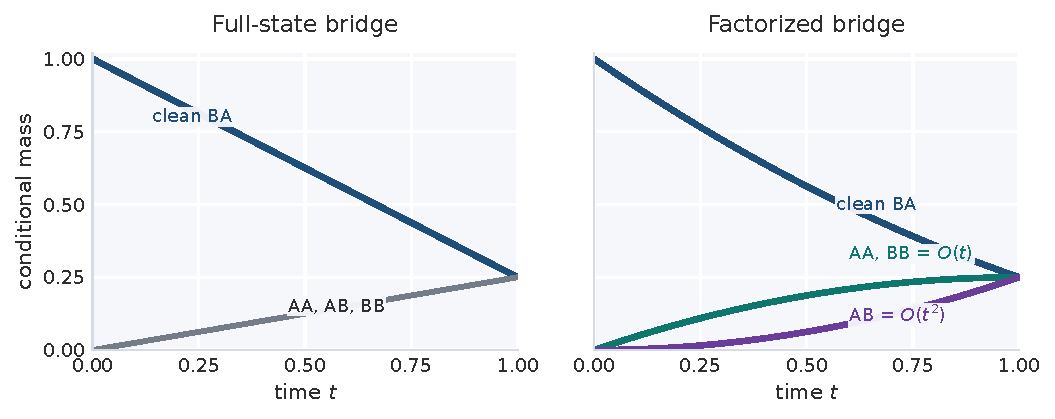
\includegraphics[width=0.92\textwidth]{figures/handouts/discrete_diffusion/fig_discrete_bridge_probabilities}
  \caption{Condition on the current bridge state \texttt{BA} in a two-token binary example.
  Under the exact full-state bridge, the alternative endpoint sequences \texttt{AA}, \texttt{AB}, and \texttt{BB} all enter at first order because one bridge time controls the whole sequence.
  Under the factorized bridge, \texttt{AA} and \texttt{BB} require one backward switch, while \texttt{AB} requires two independent switches and therefore appears only at second order.}
  \label{fig:full-vs-factorized-probabilities}
\end{figure}

This two-token toy calculation is the cleanest reason that coordinatewise marginals become sufficient after factorization.
The same distinction becomes more geometric on the two-dimensional ring example from the diffusion-models unit once we discretize the plane to a grid.
Bin the ring-mixture data law onto that grid, discretize the Gaussian reference law coordinatewise, and apply the factorized bridge \eqref{eq:factorized-mixture-path}.
At the level of marginals we still see the same kind of interpolation from the data endpoint law to the reference endpoint law.
The difference is in the sample-path geometry: the bridge no longer traces a Euclidean curve, and it instead moves by coordinatewise jumps between grid cells.

\begin{figure}[t]
  \centering
  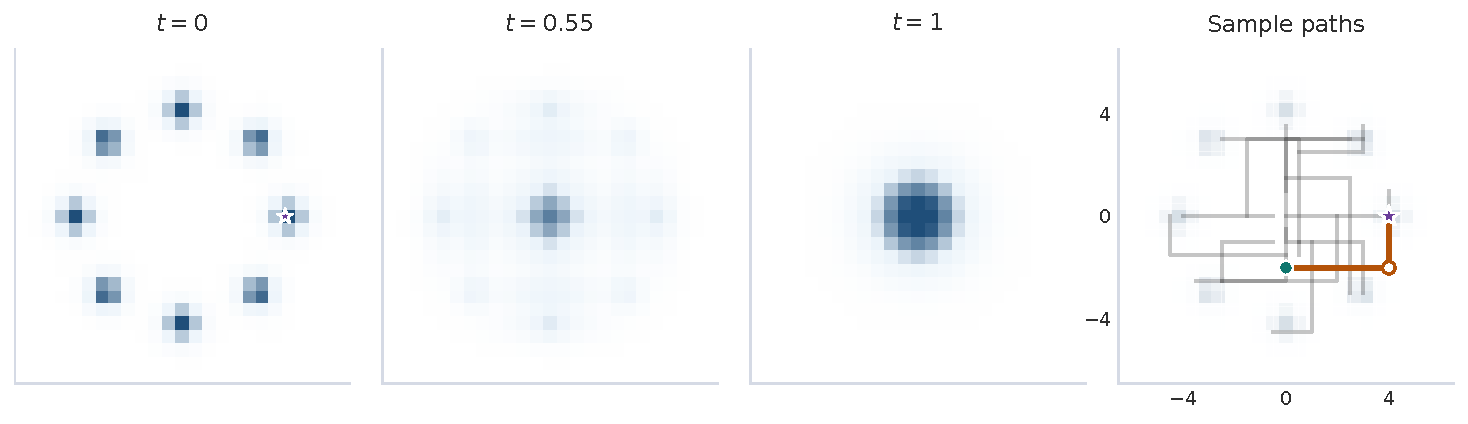
\includegraphics[width=\textwidth]{figures/handouts/discrete_diffusion/fig_discrete_spatial_bridge}
  \caption{A discretized version of the two-dimensional ring-mixture bridge.
  The first three panels show the bridge marginals on the grid at \(t=0\), \(t=0.55\), and \(t=1\).
  The last panel shows sample paths of the factorized bridge; the highlighted path starts from the starred data cell and ends at the teal reference draw.
  The marginal bridge still interpolates between the same endpoint laws, but individual paths move by one-coordinate jumps.}
  \label{fig:discrete-spatial-bridge}
\end{figure}

This is the discrete counterpart of the expectation-based picture in the continuous-state part of the diffusion-models unit.
There one learns a conditional expectation and reads off a velocity field on \(\R^2\).
Here the same bridge logic produces local jump intensities instead of a spatial vector field, which is why the finite-state description naturally passes through a generator.

For a sequence \(x\in\mathcal{V}^d\), let \(x^{j\to v}\) denote the neighbor obtained by replacing coordinate \(j\) by token \(v\).
The endpoint-conditioned generator is then as simple as possible.

\begin{proposition}[Endpoint-conditioned backward switch rule for the factorized bridge]
\label{prop:factorized-conditional-generator}
Let \(c_t\coloneqq -\dot\alpha_t/(1-\alpha_t)\), and assume \(0<\alpha_t<1\).
Then for every single-token neighbor \(x^{j\to v}\),
\begin{equation}
  Q_t^{x_0}\!\bigl(x^{j\to v}\mid x\bigr)
  =
  c_t\,\mathbf{1}\{v=x_{0,j}\}\,\mathbf{1}\{x_j\neq x_{0,j}\},
  \label{eq:factorized-conditional-generator}
\end{equation}
with diagonal chosen so that \(\sum_y Q_t^{x_0}(y\mid x)=0\).
\end{proposition}
\begin{proof}
Fix \(x_0\) and \(x\), and use the coordinatewise coupling \eqref{eq:factorized-coupling}.
If \(x_j=x_{0,j}\), then stepping backward does not require any change at coordinate \(j\).
If \(x_j\neq x_{0,j}\), conditioning on \(X_0=x_0\) and \(X_t=x\) forces \(\tau_j\le t\) and \(\Xi_j=x_j\), and the coordinate switches back exactly when \(\tau_j\in(t-h,t]\).
Therefore
\[
  \mathbb{P}(X_{t-h,j}=x_{0,j}\mid X_0=x_0,X_t=x, x_j\neq x_{0,j})
  =
  \frac{\alpha_{t-h}-\alpha_t}{1-\alpha_t}
  =
  hc_t+o(h).
\]
Independence of the switch times implies that simultaneous switches of two distinct coordinates are \(O(h^2)\), so they disappear at generator scale.
The only off-diagonal first-order moves are the backward switches in \eqref{eq:factorized-conditional-generator}.%
\end{proof}

To pass from the endpoint-conditioned generator to the marginal generator, we use the same posterior-averaging step as in the diffusion-models unit.

\begin{proposition}[Generator-level marginalization on a finite state space]
\label{prop:generator-marginalization}
Suppose
\[
  K_{t-h\mid t}(y\mid x)
  =
  \delta_x(y)+hQ_t(y\mid x)+o(h)
\]
and
\[
  K^{x_0}_{t-h\mid t}(y\mid x)
  =
  \delta_x(y)+hQ_t^{x_0}(y\mid x)+o(h)
\]
as \(h\downarrow 0\).
Then
\[
  Q_t(y\mid x)
  =
  \sum_{x_0\in S} Q_t^{x_0}(y\mid x)\,q_{0\mid t}(x_0\mid x).
\]
\end{proposition}
\begin{proof}
Apply \Cref{prop:finite-state-kernel-marginalization} with \(s=t-h\), insert the first-order expansions, subtract the common zeroth-order term \(\delta_x(y)\), divide by \(h\), and let \(h\downarrow 0\).%
\end{proof}

\begin{theorem}[Factorized generator rates depend only on coordinate marginals]
\label{thm:factorized-rates}
For the factorized mixture path \eqref{eq:factorized-mixture-path}, every off-diagonal single-token jump satisfies
\begin{equation}
  Q_t\!\bigl(x^{j\to v}\mid x\bigr)
  =
  c_t\,q_{0\mid t}\!\bigl(X_{0,j}=v\mid X_t=x\bigr),
  \qquad v\neq x_j.
  \label{eq:factorized-rate}
\end{equation}
\end{theorem}
\begin{proof}
Combine \Cref{prop:generator-marginalization} and \Cref{prop:factorized-conditional-generator}:
\[
  Q_t\!\bigl(x^{j\to v}\mid x\bigr)
  =
  \sum_{x_0\in S}
  c_t\,\mathbf{1}\{x_{0,j}=v\}\,\mathbf{1}\{x_j\neq x_{0,j}\}\,
  q_{0\mid t}(x_0\mid x).
\]
If \(v\neq x_j\), then the second indicator is automatically one on the event \(\{x_{0,j}=v\}\), so
\[
  Q_t\!\bigl(x^{j\to v}\mid x\bigr)
  =
  c_t\sum_{x_0\in S}\mathbf{1}\{x_{0,j}=v\}\,q_{0\mid t}(x_0\mid x)
  =
  c_t\,q_{0\mid t}(X_{0,j}=v\mid X_t=x).
\]
\end{proof}

If we write
\[
  \mu_{t,j}(x)\coloneqq \E[e_{X_{0,j}}\mid X_t=x]\in\R^{|\mathcal{V}|},
\]
then \Cref{thm:factorized-rates} becomes
\begin{equation}
  Q_t\!\bigl(x^{j\to v}\mid x\bigr)
  =
  c_t\,\mu_{t,j}(x)_v,
  \qquad v\neq x_j.
  \label{eq:factorized-rate-onehot}
\end{equation}
This is the cleanest statement of the simplification.
The full posterior over endpoint sequences has not disappeared.
It is still the exact posterior \(q_{0\mid t}(x_0\mid x)\) of the factorized bridge.
What the factorized bridge changes is the local move set: once only one-token backward switches are allowed at first order, the reverse rates query that posterior only through one-coordinate marginals.
So the approximation is in the bridge geometry, not in the posterior-averaging principle.
This is the generator-level reason that tokenwise classification becomes the practical training target.
The next theorem makes that precise: once the factorized bridge has been chosen, exact coordinate posteriors recover its exact reverse generator.

The full-state theorem above says that exact reverse kernels recover the correct law on any time grid.
For the factorized bridge, the parallel statement is now infinitesimal:
an ideal coordinatewise posterior model recovers the exact reverse generator of the chosen factorized bridge.
Recovering the corresponding marginal path on a time grid is then a separate numerical question, handled below by a bound in terms of accumulated one-step kernel error.

\begin{proposition}[Reverse Kolmogorov equation on a finite state space]
\label{prop:reverse-kolmogorov}
Let \(S\) be finite, let \(\pi_t\) be a differentiable path of probability mass functions on \(S\), and let \(Q_t\) be rate matrices whose entries depend continuously on \(t\).
Then the short-time relation
\[
  \pi_{t-h}(y)
  =
  \sum_{x\in S}
  \pi_t(x)\bigl[\delta_x(y)+hQ_t(y\mid x)\bigr]
  +o(h)
\]
for every \(y\in S\) is equivalent to the reverse Kolmogorov equation
\[
  -\frac{d}{dt}\pi_t(y)
  =
  \sum_{x\in S}
  \pi_t(x)\,Q_t(y\mid x),
  \qquad y\in S.
\]
Given the terminal condition \(\pi_1\), this linear ODE has a unique solution.
\end{proposition}
\begin{proof}
Because \(\sum_x \pi_t(x)\delta_x(y)=\pi_t(y)\), the short-time relation is
\[
  \pi_{t-h}(y)
  =
  \pi_t(y)
  +
  h\sum_{x\in S}\pi_t(x)\,Q_t(y\mid x)
  +
  o(h).
\]
Subtract \(\pi_t(y)\), divide by \(h\), and let \(h\downarrow 0\) to obtain the reverse Kolmogorov equation.
Conversely, if the reverse Kolmogorov equation holds, then differentiability gives
\[
  \pi_{t-h}(y)
  =
  \pi_t(y)-h\dot\pi_t(y)+o(h)
  =
  \pi_t(y)
  +
  h\sum_{x\in S}\pi_t(x)\,Q_t(y\mid x)
  +
  o(h),
\]
which is the short-time relation.
Uniqueness follows because this is a linear ODE on the finite-dimensional space \(\R^{|S|}\).%
\end{proof}

\begin{theorem}[Exact coordinate posteriors recover the factorized reverse generator]
\label{thm:factorized-infinitesimal-exactness}
For the factorized mixture path \eqref{eq:factorized-mixture-path}, suppose a model returns the exact coordinate marginals
\[
  \rho_{t,j}^\star(v\mid x)
  =
  q_{0\mid t}(X_{0,j}=v\mid X_t=x).
\]
Define the learned generator by
\[
  \hat Q_t^\star\!\bigl(x^{j\to v}\mid x\bigr)
  \coloneqq
  c_t\,\rho_{t,j}^\star(v\mid x),
  \qquad v\neq x_j,
\]
with diagonal chosen so that \(\sum_y \hat Q_t^\star(y\mid x)=0\).
Then \(\hat Q_t^\star=Q_t\), where \(Q_t\) is the exact reverse generator of the factorized bridge.
Consequently the factorized marginal path \(p_t\) is the unique solution of
\[
  -\frac{d}{dt}p_t(y)
  =
  \sum_{x\in S} p_t(x)\,\hat Q_t^\star(y\mid x),
  \qquad
  p_1 \text{ fixed},
\]
so the exact reverse CTMC for the factorized bridge transports the factorized marginal path back to \(p_0\).
\end{theorem}
\begin{proof}
The equality \(\hat Q_t^\star=Q_t\) is exactly \Cref{thm:factorized-rates}.
Because \(Q_t\) is the exact reverse generator of the factorized bridge,
\[
  K_{t-h\mid t}(y\mid x)
  =
  \delta_x(y)+hQ_t(y\mid x)+o(h).
\]
Combining this with \Cref{prop:reverse-kernels-transport} gives
\[
  p_{t-h}(y)
  =
  \sum_{x\in S}
  p_t(x)\bigl[\delta_x(y)+hQ_t(y\mid x)\bigr]
  +o(h).
\]
By \Cref{prop:reverse-kolmogorov}, the path \(p_t\) therefore solves the reverse Kolmogorov equation with generator \(Q_t=\hat Q_t^\star\).
Uniqueness gives the claim.%
\end{proof}

At this point the modeling approximation is fully visible.
The full-state sequence model and the factorized sequence model are different bridges, so they have different posteriors and different intermediate marginals.
But once the factorized bridge is chosen, \Cref{thm:factorized-infinitesimal-exactness} says that exact coordinate posteriors recover its exact reverse generator.
Equivalently, within the factorized model class the marginal dynamics are completely identified by the coordinate posteriors.
The remaining approximation is then only numerical: how accurately a discrete-time sampler tracks that reverse CTMC.

The exactness theorem above identifies the practical target immediately.
Inside the factorized bridge, learning the reverse dynamics means learning the coordinatewise posterior marginals that determine the reverse rates.
A network \(\rho_t^\theta\) therefore takes a current bridge state \(x\) and time \(t\) and outputs
\[
  \rho_{t,j}^\theta(v\mid x)
  \approx
  q_{0\mid t}(X_{0,j}=v\mid X_t=x).
\]
These outputs are still posterior objects: the full vector \(\mu_t(x)\) in the one-token case and the coordinatewise vectors \(\mu_{t,j}(x)\) in the factorized sequence case.
The statistical question is whether \(\rho_t^\theta\) learns the correct marginals.
The numerical question, which enters only after the model is trained, is how accurately a discrete-time sampler tracks the reverse CTMC determined by those marginals.
Tokenwise cross-entropy addresses the first question.

\begin{proposition}[Cross-entropy is the proper factorized objective]
\label{prop:cross-entropy-proper}
Fix \(t,x,j\), and write
\[
  \pi_j(v)\coloneqq q_{0\mid t}(X_{0,j}=v\mid X_t=x).
\]
For any candidate categorical distribution \(\rho(v)\),
\[
  \E_{V\sim \pi_j}[-\log \rho(V)]
  =
  H(\pi_j)+\operatorname{KL}(\pi_j\|\rho).
\]
Hence the expected tokenwise negative log-likelihood is minimized uniquely at \(\rho=\pi_j\).
\end{proposition}
\begin{proof}
Expand the expectation and add/subtract \(\log \pi_j(v)\):
\[
  \E_{V\sim \pi_j}[-\log \rho(V)]
  =
  \sum_v \pi_j(v)\log\frac{\pi_j(v)}{\rho(v)}
  -
  \sum_v \pi_j(v)\log \pi_j(v)
  =
  \operatorname{KL}(\pi_j\|\rho)+H(\pi_j).
\]
Only the KL term depends on \(\rho\), and it is minimized uniquely when \(\rho=\pi_j\).%
\end{proof}

The corresponding training loss is
\begin{equation}
  \mathcal{L}_{\mathrm{disc}}(\theta)
  =
  \E_{X_0\sim p_0,\; X_t\sim K_{t\mid 0}(\cdot\mid X_0),\; t\sim \mathrm{Unif}[0,1]}
  \left[
    \sum_{j=1}^d
    -\log \rho_{t,j}^\theta(X_{0,j}\mid X_t)
  \right],
  \label{eq:discrete-classification-loss}
\end{equation}
which is exactly the discrete flow-matching objective used by \citet[Eq.~(28) and Prop.~5]{gat2024discrete}.
So classification is not an extra heuristic layered on top of the bridge picture.
It is the proper scoring rule for the posterior statistics that the factorized generator actually needs.
It therefore gives the training loop directly.

\begin{algorithm}[H]
  \caption{Training a factorized discrete diffusion model}
  \label{alg:discrete-diffusion-training}
  \begin{algorithmic}[1]
    \Require Data sampler for \(p_0\), base marginals \(r_1,\dots,r_d\), schedule \(\alpha_t\), posterior network \(\rho_t^\theta\)
    \For{training steps}
      \State Sample \(x_0\sim p_0\) and \(t\sim \mathrm{Unif}[0,1]\)
      \For{\(j=1,\dots,d\) in parallel}
        \State Sample \(B_j\sim \mathrm{Bernoulli}(\alpha_t)\) and \(\Xi_j\sim r_j\)
        \If{\(B_j=1\)}
          \State Set \(x_{t,j}\gets x_{0,j}\)
        \Else
          \State Set \(x_{t,j}\gets \Xi_j\)
        \EndIf
      \EndFor
      \State Form \(x_t=(x_{t,1},\dots,x_{t,d})\)
      \State Evaluate \(\rho_{t,j}^\theta(\cdot\mid x_t)\) for all \(j\)
      \State Compute \(\ell\gets \sum_{j=1}^d -\log \rho_{t,j}^\theta(x_{0,j}\mid x_t)\)
      \State Take a gradient step on \(\ell\)
    \EndFor
  \end{algorithmic}
\end{algorithm}

Once \(\rho_t^\theta\) is trained, we obtain an approximate generator by
\[
  \hat Q_t^\theta(x^{j\to v}\mid x)
  =
  c_t\,\rho_{t,j}^\theta(v\mid x),
  \qquad v\neq x_j.
\]
An exact simulator would sample a CTMC from this generator.
For intuition, the simplest approximation is a parallel Euler step, which keeps the \(O(h)\) single-token events and ignores the \(O(h^2)\) simultaneous jumps over a step of size \(h\).

\begin{algorithm}[H]
  \caption{Euler sampling for the learned CTMC}
  \label{alg:discrete-diffusion-sampling}
  \begin{algorithmic}[1]
    \Require Base sampler for \(p_1\), time grid \(1=t_K>\cdots>t_0=0\), schedule factor \(c_t\), learned posterior network \(\rho_t^\theta\)
    \State Sample \(X_{t_K}\sim p_1\)
    \For{\(k=K,K-1,\dots,1\)}
      \State Set \(t\gets t_k\), \(h\gets t_k-t_{k-1}\), \(x\gets X_{t_k}\)
      \State Evaluate \(\rho_{t,j}^\theta(\cdot\mid x)\) for all coordinates \(j\)
      \For{\(j=1,\dots,d\) in parallel}
        \For{each \(v\neq x_j\)}
          \State \(\tilde p_j(v\mid x_j)\gets h\,c_t\,\rho_{t,j}^\theta(v\mid x)\)
        \EndFor
        \State \(\tilde p_j(x_j\mid x_j)\gets 1-h\sum_{v\neq x_j} c_t\,\rho_{t,j}^\theta(v\mid x)\)
        \State Sample \(X_{t_{k-1},j}\sim \mathrm{Categorical}(\tilde p_j(\cdot\mid x_j))\)
      \EndFor
      \State Set \(X_{t_{k-1}}\gets (X_{t_{k-1},1},\dots,X_{t_{k-1},d})\)
    \EndFor
    \State \Return \(X_{t_0}\)
  \end{algorithmic}
\end{algorithm}

Euler is only the time discretization.
The structural approximation happened earlier, when we replaced the full \(|\mathcal{V}|^d\)-state model by the factorized local bridge.
That distinction matters because classification is learning the posterior statistics needed by the chosen local generator, while Euler is only approximating the CTMC generated by those statistics.
For the per-coordinate categorical probabilities in \Cref{alg:discrete-diffusion-sampling} to be valid, we choose a grid fine enough that
\[
  h\,c_t\le 1
\]
at every step; this guarantees \(\tilde p_j(x_j\mid x_j)\ge 0\).
With that understood, the Euler sampler is one concrete family of approximate kernels \(\hat K_k\).

This isolates the remaining numerical question.
Fix a time grid and let \(K_k=K_{t_{k-1}\mid t_k}\) denote the exact reverse kernels of the factorized bridge on that grid.
Any practical sampler, including \Cref{alg:discrete-diffusion-sampling}, replaces \(K_k\) by approximate kernels \(\hat K_k\).
The only question is how those one-step kernel errors accumulate.

\begin{proposition}[Accumulated one-step kernel error controls gridwise marginal error]
\label{prop:accumulated-kernel-error}
Fix a decreasing grid \(1=t_K>\cdots>t_0=0\).
Let \(K_k=K_{t_{k-1}\mid t_k}\) be the exact reverse kernels of a bridge path, and let \(\hat K_k\) be any approximate reverse kernels on the same grid.
Start both chains from the same terminal law,
\[
  p_K=\hat p_K=p_1,
\]
and define
\[
  p_{k-1}=p_k K_k,
  \qquad
  \hat p_{k-1}=\hat p_k \hat K_k,
  \qquad k=K,\dots,1.
\]
For each step set
\[
  \varepsilon_k
  \coloneqq
  \sup_{x\in S}
  \sum_{y\in S}
  \bigl|\hat K_k(y\mid x)-K_k(y\mid x)\bigr|.
\]
Then for every \(m=0,\dots,K\),
\[
  \|\hat p_m-p_m\|_1
  \le
  \sum_{k=m+1}^K \varepsilon_k.
\]
In particular,
\[
  \|\hat p_0-p_0\|_1
  \le
  \sum_{k=1}^K \varepsilon_k.
\]
\end{proposition}
\begin{proof}
If \(m\) is any signed mass function on \(S\) and \(K\) is any Markov kernel, then
\[
  \|mK\|_1
  =
  \sum_{y\in S}
  \left|\sum_{x\in S} m(x)\,K(y\mid x)\right|
  \le
  \sum_{x\in S}|m(x)|\sum_{y\in S}K(y\mid x)
  =
  \|m\|_1.
\]
So Markov kernels are \(\ell_1\)-contractive.
Now
\[
  \hat p_{k-1}-p_{k-1}
  =
  (\hat p_k-p_k)\hat K_k
  +
  p_k(\hat K_k-K_k),
\]
and therefore
\[
  \|\hat p_{k-1}-p_{k-1}\|_1
  \le
  \|(\hat p_k-p_k)\hat K_k\|_1
  +
  \|p_k(\hat K_k-K_k)\|_1
  \le
  \|\hat p_k-p_k\|_1+\varepsilon_k.
\]
Iterating backward from \(\|\hat p_K-p_K\|_1=0\) gives the stated bound for every grid point.%
\end{proof}

\begin{corollary}[Small-step recovery of the factorized marginal path]
\label{cor:factorized-small-step-recovery}
Consider the factorized bridge \eqref{eq:factorized-mixture-path}, and suppose the learned posterior model is ideal so that \(\rho_{t,j}^\star(v\mid x)=q_{0\mid t}(X_{0,j}=v\mid X_t=x)\).
For each grid \(\Pi^{(n)}=\{1=t^{(n)}_{K_n}>\cdots>t^{(n)}_0=0\}\), let \(K_k^{(n)}\) be the exact reverse kernels of the factorized bridge and let \(\hat K_k^{(n)}\) be any approximate kernels built from those exact coordinate marginals.
If
\[
  \sum_{k=1}^{K_n}
  \sup_{x\in S}\sum_{y\in S}
  \bigl|\hat K_k^{(n)}(y\mid x)-K_k^{(n)}(y\mid x)\bigr|
  \longrightarrow 0
  \qquad\text{as } n\to\infty,
\]
then the approximate reverse chain converges at every grid point to the marginal path of the factorized bridge.
In particular,
\[
  \|\hat p_0^{(n)}-p_0\|_1\to 0.
\]
\end{corollary}
\begin{proof}
By \Cref{thm:factorized-infinitesimal-exactness}, the exact coordinate marginals recover the exact reverse generator of the factorized bridge.
Hence the exact reverse kernels \(K_k^{(n)}\) are the correct kernels for that bridge on the grid \(\Pi^{(n)}\).
Applying \Cref{prop:accumulated-kernel-error} to each grid gives the result.%
\end{proof}

This is the precise sense in which the practical factorized sampler becomes exact.
It does not say that the factorized bridge reproduces the exact full-state bridge on \(\mathcal{V}^d\); that modeling approximation was made earlier.
It says that once the factorized bridge is chosen, exact coordinate posteriors plus vanishing one-step kernel error recover its marginal path, and therefore its data endpoint \(p_0\), in the many-step limit.

\begin{exercise}[Reading factorized reverse rates]
\label{ex:reading-factorized-rates}
Stay inside the factorized bridge on the binary vocabulary \(\mathcal{V}=\{A,B\}\), and let the current bridge state be \(x=\texttt{BA}\).
Suppose
\[
  q_{0\mid t}(X_{0,1}=A\mid X_t=x)=0.6,
  \qquad
  q_{0\mid t}(X_{0,1}=B\mid X_t=x)=0.4,
\]
\[
  q_{0\mid t}(X_{0,2}=A\mid X_t=x)=0.2,
  \qquad
  q_{0\mid t}(X_{0,2}=B\mid X_t=x)=0.8,
\]
and \(c_t=3\).
\begin{enumerate}[leftmargin=*]
  \item Compute the off-diagonal reverse rates from \(\texttt{BA}\) to \(\texttt{AA}\) and to \(\texttt{BB}\).
  \item Compute the diagonal entry \(Q_t(\texttt{BA}\mid \texttt{BA})\).
  \item Explain why no table of joint probabilities \(q_{0\mid t}(X_{0,1},X_{0,2}\mid X_t=x)\) appears in these rates.
\end{enumerate}
\end{exercise}
\SolutionBox[10]{The neighbor \(\texttt{AA}\) is \(x^{1\to A}\), so \eqref{eq:factorized-rate} gives
\[
  Q_t(\texttt{AA}\mid \texttt{BA})
  =
  3\cdot q_{0\mid t}(X_{0,1}=A\mid X_t=x)
  =
  3(0.6)
  =
  1.8.
\]
Similarly \(\texttt{BB}=x^{2\to B}\), so
\[
  Q_t(\texttt{BB}\mid \texttt{BA})
  =
  3\cdot q_{0\mid t}(X_{0,2}=B\mid X_t=x)
  =
  3(0.8)
  =
  2.4.
\]
The row sum must vanish, hence
\[
  Q_t(\texttt{BA}\mid \texttt{BA})=-(1.8+2.4)=-4.2.
\]
No joint two-token table appears because the factorized bridge only allows one-token backward switches at first order.
Once the local move set is restricted to \(x^{j\to v}\), the reverse generator queries the posterior only through one-coordinate marginals.}

\begin{exercise}[Why only one-token jumps survive at first order]
\label{ex:one-token-jumps}
Use the factorized coupling \eqref{eq:factorized-coupling}.
Fix two distinct coordinates \(j\neq k\), and suppose both are currently away from their \(t=0\) endpoint values, so \(x_j\neq x_{0,j}\) and \(x_k\neq x_{0,k}\).
\begin{enumerate}[leftmargin=*]
  \item Show that
  \[
    \mathbb{P}\bigl(X_{t-h,j}=x_{0,j},\,X_{t-h,k}=x_{0,k}\mid X_0=x_0,\;X_t=x\bigr)
    =
    O(h^2).
  \]
  \item Explain why this implies that two-token jumps disappear at generator scale.
  \item Conclude that the generator-level reverse object only needs the coordinate marginals \(q_{0\mid t}(X_{0,j}=v\mid X_t=x)\), not simultaneous two-token switch probabilities.
\end{enumerate}
\end{exercise}
\SolutionBox[12]{Conditionally on \(X_0=x_0\) and \(X_t=x\), each coordinate that is away from its \(t=0\) endpoint switches back exactly when its switch time lies in \((t-h,t]\).
For one coordinate this has probability
\[
  \mathbb{P}(\tau_j\in (t-h,t]\mid \tau_j\le t)
  =
  hc_t+o(h).
\]
Because the switch times are independent across coordinates,
\begin{align*}
  &\mathbb{P}\bigl(X_{t-h,j}=x_{0,j},\,X_{t-h,k}=x_{0,k}\mid X_0=x_0,\;X_t=x\bigr) \\
  &\qquad=
  \mathbb{P}(\tau_j\in (t-h,t]\mid \tau_j\le t)\,
  \mathbb{P}(\tau_k\in (t-h,t]\mid \tau_k\le t)
  =
  \bigl(hc_t+o(h)\bigr)^2
  =
  O(h^2).
\end{align*}
After dividing by \(h\) to form the generator, any \(O(h^2)\) event vanishes.
So the first-order reverse dynamics can only move along one-token neighbors.
That is the structural reason the generator depends only on one-coordinate posterior marginals: simultaneous two-token switch probabilities never appear at first order.}

\subsection{Masked diffusion as a sharpened special case}
\label{subsec:masked-diffusion}

Masked diffusion makes the factorized story even cleaner by collapsing the reference law to a point mass.
It is not a new approximation layer; it is a particularly simple factorized bridge.
Adjoin an absorbing token \([\mathrm{MASK}]\notin\mathcal{V}\), set \(r_j=\delta_{[\mathrm{MASK}]}\) for every coordinate, and let
\[
  p_1=\delta_{[\mathrm{MASK}]^d}.
\]
Each coordinate now either keeps the \(t=0\) endpoint token or is replaced by \([\mathrm{MASK}]\).
Equivalently, the factorized bridge becomes
\begin{equation}
  K_{t\mid 0}(x\mid x_0)
  =
  \prod_{j=1}^d
  \Bigl[
    \alpha_t\,\delta_{x_{0,j}}(x_j)
    +
    (1-\alpha_t)\,\delta_{[\mathrm{MASK}]}(x_j)
  \Bigr].
  \label{eq:masked-factorized-bridge}
\end{equation}
This is the absorbing-mask version of the same factorized bridge picture.

\begin{corollary}[Revealed coordinates are already solved]
\label{cor:masked-revealed}
If \(X_{t,j}\neq [\mathrm{MASK}]\), then
\[
  q_{0\mid t}(X_{0,j}=X_{t,j}\mid X_t)=1
\]
and
\[
  q_{0\mid t}(X_{0,j}=v\mid X_t)=0
  \qquad \text{for } v\neq X_{t,j}.
\]
\end{corollary}
\begin{proof}
Under the masked bridge, a revealed token can only arise by keeping the \(t=0\) endpoint token.
So any endpoint sequence compatible with \(X_t\) must satisfy \(X_{0,j}=X_{t,j}\).%
\end{proof}

The second simplification is specific to the absorbing mask.
Once the current state tells us which coordinates are revealed and which are masked, the schedule factor contributes the same scalar weight to every compatible endpoint sequence.
After normalization it cancels.

\begin{proposition}[The masked posterior does not depend on time]
\label{prop:masked-time-independent}
Let \(x\in(\mathcal{V}\cup\{[\mathrm{MASK}]\})^d\), and define
\[
  U(x)\coloneqq \{j:x_j\neq [\mathrm{MASK}]\},
  \qquad
  M(x)\coloneqq \{j:x_j=[\mathrm{MASK}]\}.
\]
For the masked factorized bridge,
\begin{equation}
  K_{t\mid 0}(x\mid x_0)
  =
  \alpha_t^{|U(x)|}(1-\alpha_t)^{|M(x)|}
  \prod_{j\in U(x)} \mathbf{1}\{x_{0,j}=x_j\}.
  \label{eq:masked-likelihood-factor}
\end{equation}
Consequently,
\begin{equation}
  q_{0\mid t}(x_0\mid x)
  \propto
  p_0(x_0)\prod_{j\in U(x)}\mathbf{1}\{x_{0,j}=x_j\},
  \label{eq:masked-posterior-t-free}
\end{equation}
so the posterior depends on the masked pattern and the revealed tokens, but not on \(t\).
\end{proposition}
\begin{proof}
Each revealed coordinate contributes \(\alpha_t\,\mathbf{1}\{x_{0,j}=x_j\}\), and each masked coordinate contributes \(1-\alpha_t\).
Multiplying over coordinates gives \eqref{eq:masked-likelihood-factor}.
Bayes' rule then yields
\[
  q_{0\mid t}(x_0\mid x)
  \propto
  p_0(x_0)\,\alpha_t^{|U(x)|}(1-\alpha_t)^{|M(x)|}
  \prod_{j\in U(x)}\mathbf{1}\{x_{0,j}=x_j\}.
\]
The schedule factor does not depend on \(x_0\), so it cancels during normalization.%
\end{proof}

Equivalently, once we observe a masked row \(x\), the posterior is just the data law \(p_0\) renormalized on the set of endpoint sequences that agree with the revealed coordinates \(x_{U(x)}\).
The only role of the forward schedule is to contribute the common scalar \(\alpha_t^{|U(x)|}(1-\alpha_t)^{|M(x)|}\), and that scalar disappears when we normalize.

This is the posterior explanation for two familiar implementation choices.
First, the network can ignore time in the purely masked setting because the target posterior is time-independent \citep[Prop.~6 and App.~E.8]{gat2024discrete}.
Second, the loss can be restricted to masked positions because revealed coordinates already have degenerate posteriors.
That is exactly why the absorbing mask collapses the generic bridge problem to ordinary prediction on the masked coordinates.

\begin{exercise}[Why the schedule cancels in the masked case]
\label{ex:masked-cancel}
Fix a masked bridge state \(x\), and let \(U(x)\) and \(M(x)\) denote its revealed and masked coordinates.
\begin{enumerate}[leftmargin=*]
  \item Starting from \eqref{eq:masked-likelihood-factor}, show that every endpoint sequence compatible with the revealed coordinates receives the same factor
  \[
    \alpha_t^{|U(x)|}(1-\alpha_t)^{|M(x)|}.
  \]
  \item Use Bayes' rule to derive \eqref{eq:masked-posterior-t-free}.
  \item For a masked coordinate \(j\in M(x)\), prove that for every token \(v\in\mathcal{V}\),
  \[
    q_{0\mid t}(X_{0,j}=v\mid X_t=x)
    =
    \mathbb{P}_{X_0\sim p_0}\bigl(X_{0,j}=v \mid X_{0,U(x)}=x_{U(x)}\bigr).
  \]
  \item Why can the loss be restricted to masked positions?
\end{enumerate}
\end{exercise}
\SolutionBox[14]{By \eqref{eq:masked-likelihood-factor},
\[
  K_{t\mid 0}(x\mid x_0)
  =
  \alpha_t^{|U(x)|}(1-\alpha_t)^{|M(x)|}
  \prod_{i\in U(x)}\mathbf{1}\{x_{0,i}=x_i\}.
\]
So every endpoint sequence \(x_0\) compatible with the revealed coordinates gets the same schedule-dependent factor, and every incompatible sequence gets likelihood zero.
Bayes' rule gives
\[
  q_{0\mid t}(x_0\mid x)
  \propto
  p_0(x_0)\,
  \alpha_t^{|U(x)|}(1-\alpha_t)^{|M(x)|}
  \prod_{i\in U(x)}\mathbf{1}\{x_{0,i}=x_i\}.
\]
The schedule factor does not depend on \(x_0\), so it cancels during normalization:
\[
  q_{0\mid t}(x_0\mid x)
  \propto
  p_0(x_0)\prod_{i\in U(x)}\mathbf{1}\{x_{0,i}=x_i\}.
\]
Therefore, for \(j\in M(x)\),
\[
  q_{0\mid t}(X_{0,j}=v\mid X_t=x)
  =
  \mathbb{P}_{X_0\sim p_0}\bigl(X_{0,j}=v \mid X_{0,U(x)}=x_{U(x)}\bigr).
\]
Revealed positions can be dropped from the loss because their posteriors are already point masses by \Cref{cor:masked-revealed}; only the masked coordinates still carry uncertainty.}

\subsection{Connection back to the Euclidean expectation lens}
\label{subsec:euclidean-connection}

The bridge-first parallel with the Euclidean setting can be written explicitly:
\[
  \begin{aligned}
    \text{Euclidean bridge:}\qquad
    &\text{learn }
    \E[\dot X_t\mid X_t=x]
    \text{ or }
    \E[X_0\mid X_t=x].\\[0.35em]
    \text{Full finite-state bridge on }S:\qquad
    &\text{learn }
    \E[e_{X_0}\mid X_t=x]
    =
    q_{0\mid t}(\cdot\mid x).\\[0.35em]
    \text{Factorized bridge on }\mathcal{V}^d:\qquad
    &\text{learn }
    \E[e_{X_{0,j}}\mid X_t=x]
    =
    q_{0\mid t}(X_{0,j}=\cdot\mid X_t=x)
    \text{ for each }j.
  \end{aligned}
\]

The Euclidean model cannot represent the full posterior by a finite-dimensional simplex vector, so it learns the conditional expectations under that posterior that are infinitesimally sufficient for the marginal dynamics.
The one-token discrete model can represent the full posterior exactly, because a one-hot expectation on a finite set is already a probability vector.
The factorized sequence model makes the parallel tractability move: it keeps the posterior-averaging principle but chooses a local jump geometry whose infinitesimal rates depend only on coordinatewise posterior marginals.
Within that factorized model, those marginals still recover the correct reverse dynamics and therefore the correct endpoint law \(p_0\).
That is the precise sense in which practical discrete diffusion reduces to classification.

So the clean conclusion is not that discrete diffusion secretly stops being distributional.
It is the opposite.
The exact finite-state story is fully distributional from the start, and tokenwise classification appears only after we decide to approximate the full sequence model by a factorized local bridge.

\begin{exercise}[Classify the bridge]
\label{ex:classify-the-bridge}
For each scenario below, decide whether the tokenwise-classification reduction developed above is exact at the generator level, exact only in the masked/time-independent special case, or only approximate.
In each case, identify the first-order reverse move set and the first model change you would try if that reduction fails.
\begin{enumerate}[leftmargin=*]
  \item A one-token categorical bridge with a known schedule.
  \item A factorized sequence bridge with independent switch times.
  \item A masked bridge where the network is trained only on masked positions.
  \item A coupled bridge in which two-token moves occur at first order.
\end{enumerate}
\end{exercise}
\SolutionBox[14]{For the one-token categorical bridge, classification is exact at the generator level:
the reverse chain can jump from the current token \(x\) to any token \(v\neq x\), and the rates are exactly the posterior coordinates \(q_{0\mid t}(X_0=v\mid X_t=x)\).
For the factorized sequence bridge, classification is again exact at the generator level:
the first-order move set consists of one-token neighbors \(x^{j\to v}\), and the corresponding rates are exactly the coordinate marginals \(q_{0\mid t}(X_{0,j}=v\mid X_t=x)\).
For the masked bridge, this is the masked/time-independent special case of the factorized bridge, so the reduction remains exact at the generator level:
the uncertain moves live only on masked coordinates, the posterior ignores \(t\), and training can therefore be restricted to masked positions whose posteriors are not already degenerate.
For a coupled bridge with two-token moves at first order, classification is only approximate.
The reverse generator now needs block moves or other nonlocal jumps, so a tokenwise classifier is missing the first-order object itself.
The first fix is to enlarge the learned reverse object, for example by modeling blockwise posteriors or a richer reverse kernel that can score coupled edits.}

\subsection{Other discrete variants}
\label{subsec:other-discrete-variants}

The discussion above focused on one model class:
a factorized bridge, its reverse CTMC, and the discrete flow-matching objective that learns the posterior marginals needed by that generator.
That is the cleanest setup for developing the distributional picture without fragmentation.

Other named discrete diffusion models can mostly be understood as changing one of three ingredients while keeping the same bridge-first logic.
The uniform multinomial kernel of \citet[\S4]{hoogeboom2021argmax} is the basic one-token categorical instance of this story.
Absorbing-mask models are the sharpened special case from \Cref{subsec:masked-diffusion}; in discrete time this is the absorbing-state construction in \citet[\S3.1]{austin2021structured}, while in the present flow-matching setup the posterior simplification is exactly the one stated in \citep[Prop.~6 and App.~E.8]{gat2024discrete}.
Richer D3PM-style constructions play the same role by changing the one-token forward corruption kernel in the discrete-time model \citep[\S3.1--3.3]{austin2021structured}; in the bridge-first view used here, that changes the local geometry while leaving the posterior-averaging principle intact.

So the real conceptual distinction is not between many separate algorithms.
It is between the exact full-state bridge, the tractable factorized bridge, and the numerical schemes used to approximate reverse-time sampling once that bridge has been chosen.
Carried back to the main notes, the lesson is the same as in the Euclidean diffusion story: choose a bridge, identify the conditional object that is sufficient for reverse-time transport, and then ask which tractable approximation preserves that sufficiency.
The discrete setting is simply the case where, for some bridges, that conditional object is a literal posterior vector rather than a lower-dimensional summary.

\bibliographystyle{plainnat}
\makeatletter
\begingroup
\let\input@path\@empty
\IfFileExists{references.bib}{%
  \gdef\stat221bibpath{references}%
}{%
  \IfFileExists{../references.bib}{%
    \gdef\stat221bibpath{../references}%
  }{%
    \gdef\stat221bibpath{../../references}%
  }%
}
\endgroup
\makeatother
\bibliography{\stat221bibpath}

\end{document}
"
%   (Low-level direct build: if you invoke latexmk manually, set -jobname to the
%    titled output so the compiled PDF matches the standard naming scheme.)
\newif\ifshowsolutions
\showsolutionsfalse
\ifdefined\STATshowsolutions
  \showsolutionstrue
\fi
\ifcsname STAT221SOLUTIONS\endcsname
  \showsolutionstrue
\fi

% Solutions/workspace boxes (controlled by \ifshowsolutions).
% Usage: \SolutionBox[<workspace lines>]{<solution body>}
\newcommand{\SolutionBox}[2][10]{%
  \ifshowsolutions
    \begin{tcolorbox}[stat221panelgray,title={Solution}]
    #2
    \end{tcolorbox}
  \else
    \begin{tcolorbox}[stat221panelgray,unbreakable,title={Workspace}]
    \vspace{#1\baselineskip}
    \end{tcolorbox}
  \fi
}

\title{Discrete diffusion as posterior learning}
\author{}
\date{}

\begin{document}
\maketitle

\section[Discrete diffusion as posterior learning]{Discrete diffusion as posterior learning}
\label{sec:discrete-posterior-learning}

Fix a finite state space \(S\).
This handout takes the diffusion unit's bridge-first viewpoint and specializes it to a setting where the reverse-time object can sometimes be represented exactly.
The central ingredients are the endpoint laws \(p_0\) and \(p_1\), the chosen bridge \(K_{t\mid 0}(\cdot\mid x_0)\), and the endpoint posterior \(q_{0\mid t}\) induced by that bridge.
In finite state spaces the resulting question becomes unusually clean: when does reverse sampling reduce to classification, and when does tractability require a change in the bridge itself?

Let \(p_0\) be the data law on \(S\), let \(p_1\) be a reference law, and let \(K_{t\mid 0}(\cdot\mid x_0)\) be a conditional probability path with
\[
  K_{0\mid 0}(\cdot\mid x_0)=\delta_{x_0},
  \qquad
  K_{1\mid 0}(\cdot\mid x_0)=p_1.
\]
Averaging over \(X_0\sim p_0\) gives the marginal law \(p_t\), and Bayes' rule gives the endpoint posterior
\[
  q_{0\mid t}(x_0\mid x)
  =
  \frac{p_0(x_0)K_{t\mid 0}(x\mid x_0)}{p_t(x)}.
\]
If we knew this posterior exactly, reverse sampling would be straightforward:
sample an endpoint from \(q_{0\mid t}(\cdot\mid x)\) and then take the bridge step conditioned on that endpoint.
This is the finite-state specialization of the posterior-averaging mechanism developed in the diffusion-models unit.

When \(S\) is small, the one-hot conditional expectation \(\E[e_{X_0}\mid X_t=x]\) is already the full posterior vector \(q_{0\mid t}(\cdot\mid x)\).
For a one-token vocabulary model that means classifier outputs can represent the exact reverse-time object.
For the full sequence state space \(S=\mathcal{V}^d\), the same statement remains true but becomes computationally useless because the simplex has size \(|\mathcal{V}|^d\).
Practical discrete diffusion therefore changes the bridge, not the posterior-averaging principle: it replaces the exact full-sequence bridge by a coordinatewise bridge whose reverse generator depends only on coordinatewise posterior marginals.
The discussion below follows that progression from the exact finite-state bridge to the exact full-sequence model and then to the factorized sequence bridge used in practice.

\subsection{Exact posterior learning on a finite state space}
\label{subsec:finite-state-full-posterior}

We now specialize the bridge and posterior notation of the diffusion-models unit to a finite state space \(S\).
Let \(p_0\) be the data law, \(p_1\) a reference law, and
\[
  K_{t\mid 0}(\cdot\mid x_0),
  \qquad
  K_{0\mid 0}(\cdot\mid x_0)=\delta_{x_0},
  \qquad
  K_{1\mid 0}(\cdot\mid x_0)=p_1
\]
is a conditional probability path.
The corresponding marginal path is
\[
  p_t(x)=\sum_{x_0\in S} p_0(x_0)\,K_{t\mid 0}(x\mid x_0),
\]
and Bayes' rule gives the posterior over the \(t=0\) endpoint states,
\[
  q_{0\mid t}(x_0\mid x)
  =
  \frac{p_0(x_0)K_{t\mid 0}(x\mid x_0)}{p_t(x)}.
\]
This formula is understood on the support of \(p_t\), that is, for states \(x\) with \(p_t(x)>0\).

In the Euclidean development of the diffusion-models unit, one passes from the full posterior to conditional expectations that are infinitesimally sufficient.
On a finite state space, a one-hot embedding of the \(t=0\) endpoint loses no information, so the same conditional expectation is the full posterior itself.
Suppressing the dependence on \(S\), write \(e_z\in\R^{|S|}\) for the basis vector indexed by \(z\in S\).

\begin{proposition}[The one-hot conditional expectation is the full posterior]
\label{prop:full-state-onehot}
Define
\[
  \mu_t(x)\coloneqq \E[e_{X_0}\mid X_t=x]\in\R^{|S|}.
\]
Then
\begin{equation}
  \mu_t(x)_z
  =
  q_{0\mid t}(X_0=z\mid X_t=x),
  \qquad z\in S.
  \label{eq:full-state-onehot}
\end{equation}
\end{proposition}
\begin{proof}
Because \(e_{X_0}=e_z\) on the event \(\{X_0=z\}\),
\[
  \mu_t(x)
  =
  \sum_{z\in S} e_z\,\mathbb{P}(X_0=z\mid X_t=x).
\]
Taking the \(z\)th coordinate gives \eqref{eq:full-state-onehot}.%
\end{proof}

\Cref{prop:full-state-onehot} is the finite-state version of the Euclidean expectation reduction, except that here the reduction is exact.
In Euclidean space, quantities like \(\E[\dot X_t\mid X_t=x]\) or \(\E[X_0\mid X_t=x]\) summarize a richer posterior.
For a finite state space, the one-hot expectation \(\E[e_{X_0}\mid X_t=x]\) already is the posterior.
When \(S=\mathcal{V}\), a classifier over the vocabulary is therefore an exact posterior model.

\begin{figure}[t]
  \centering
  \begin{tikzpicture}[font=\small]
  \tikzset{
    panel/.style={
      rounded corners=7pt,
      draw=stat221Gray!30,
      fill=stat221GrayLight,
      line width=0.85pt,
    },
    infobox/.style={
      rounded corners=5pt,
      draw=stat221Blue!55!black,
      fill=white,
      line width=0.85pt,
      inner sep=8pt,
      text width=4.6cm,
      align=left,
    },
    coordlabel/.style={
      font=\footnotesize,
      fill=white,
      inner sep=1.5pt,
      text=stat221Gray,
    },
  }

  \path[use as bounding box] (-0.1,-0.1) rectangle (13.9,5.25);
  \draw[panel] (0,0) rectangle (13.7,4.95);

  \node[font=\small\bfseries,text=stat221Gray] at (3.10,4.58)
    {The posterior lives in the simplex};
  \node[font=\small\bfseries,text=stat221Gray] at (10.28,4.58)
    {Its coordinates are the reverse rates};

  \coordinate (A) at (0.95,0.78);
  \coordinate (B) at (5.85,0.78);
  \coordinate (C) at (3.40,3.95);
  \coordinate (P) at (2.76,1.50);

  \fill[white] (A) -- (B) -- (C) -- cycle;
  \draw[stat221Gray!70,line width=1.05pt] (A) -- (B) -- (C) -- cycle;

  % Constant-coordinate lines through the posterior point.
  \draw[stat221Blue!70!black,densely dashed,line width=1.0pt]
    ($(A)!0.5!(B)$) -- ($(A)!0.5!(C)$);
  \draw[stat221Green!70!black,densely dashed,line width=1.0pt]
    ($(B)!0.3!(A)$) -- ($(B)!0.3!(C)$);
  \draw[stat221Purple!70!black,densely dashed,line width=1.0pt]
    ($(C)!0.2!(A)$) -- ($(C)!0.2!(B)$);

  \filldraw[fill=stat221BlueLight,draw=stat221Blue!70!black,line width=0.9pt] (A) circle (0.16);
  \filldraw[fill=stat221GreenLight,draw=stat221Green!70!black,line width=0.9pt] (B) circle (0.16);
  \filldraw[fill=stat221PurpleLight,draw=stat221Purple!70!black,line width=0.9pt] (C) circle (0.16);
  \node[font=\small\bfseries,text=stat221Blue!75!black] at ($(A)+(-0.38,-0.28)$) {\(A\)};
  \node[font=\small\bfseries,text=stat221Green!60!black] at ($(B)+(0.38,-0.28)$) {\(B\)};
  \node[font=\small\bfseries,text=stat221Purple!60!black] at ($(C)+(0.00,0.35)$) {\(C\)};

  \filldraw[fill=stat221Gray,draw=white,line width=0.9pt] (P) circle (0.12);
  \draw[stat221Gray!60,line width=0.8pt] (P) -- +(0.55,0.55);
  \node[font=\small,text=stat221Gray,align=left] at ($(P)+(0.68,0.68)$)
    {\(\mu_t(x)\)};
  \node[font=\scriptsize,text=stat221Gray,align=left] at ($(P)+(0.92,0.28)$)
    {\(=q_{0\mid t}(\cdot\mid x)\)};

  \node[coordlabel,text=stat221Blue!75!black] at (1.80,2.38) {\(A=0.5\)};
  \node[coordlabel,text=stat221Green!60!black] at (4.85,2.10) {\(B=0.3\)};
  \node[coordlabel,text=stat221Purple!60!black] at (2.35,1.02) {\(C=0.2\)};

  \node[infobox] (info) at (10.30,2.45) {%
    \(\displaystyle \mu_t(x)=(0.5,\,0.3,\,0.2)\)

    \vspace{0.45em}
    \textcolor{stat221Blue!75!black}{\(Q_t^{\mathrm{rev}}(A\mid x)=0.5\,c_t\)}

    \textcolor{stat221Green!60!black}{\(Q_t^{\mathrm{rev}}(B\mid x)=0.3\,c_t\)}

    \textcolor{stat221Purple!60!black}{\(Q_t^{\mathrm{rev}}(C\mid x)=0.2\,c_t\)}

    \vspace{0.55em}
    The reverse generator is \(c_t\) times these coordinates.};
\end{tikzpicture}

  \caption{In the one-token setting, the posterior is literally a point in the simplex over endpoint states.
  Learning that point is genuinely distributional, and the reverse generator just rescales its coordinates by the common jump rate \(c_t\).}
  \label{fig:one-token-distributional}
\end{figure}

This is the discrete analogue of the conditional-versus-marginal story in the diffusion-models unit.
We observe the current bridge state \(X_t=x\), infer the conditional law of the endpoint \(X_0\mid X_t=x\), and then use a sampled endpoint to take the reverse bridge step.
The only difference from the Euclidean case is that on a finite set the relevant posterior can sometimes be represented exactly by a finite vector.

Operationally, an exact finite-state bridge can therefore be sampled in two stages.
Given a current state \(x_t\) and an earlier time \(s<t\), first draw an endpoint and then draw from the bridge conditioned on that endpoint:
\[
  \tilde X_0\sim q_{0\mid t}(\cdot\mid x_t),
  \qquad
  X_s\sim K^{\tilde X_0}_{s\mid t}(\cdot\mid x_t).
\]
Marginalizing \(\tilde X_0\) recovers the exact earlier-time kernel \(K_{s\mid t}(\cdot\mid x_t)\).
So in the one-token case there is no approximation to explain away: infer the full conditional law of \(X_0\mid X_t=x_t\), sample an endpoint from it, and then take the exact bridge step conditioned on that sample.

\begin{proposition}[Endpoint-conditioned bridge marginalization on a finite state space]
\label{prop:finite-state-kernel-marginalization}
Let \(0\le s\le t\le 1\).
Write \(K^{x_0}_{s\mid t}(\cdot\mid x_t)\) for the bridge kernel from time \(t\) to the earlier time \(s\) conditioned on the endpoint \(X_0=x_0\).
Then
\[
  K_{s\mid t}(y\mid x_t)
  =
  \sum_{x_0\in S}
  K^{x_0}_{s\mid t}(y\mid x_t)\,
  q_{0\mid t}(x_0\mid x_t).
\]
\end{proposition}
\begin{proof}
For states \(x_t\) with \(p_t(x_t)>0\), the law of total probability gives
\[
  \mathbb{P}(X_s=y\mid X_t=x_t)
  =
  \sum_{x_0\in S}
  \mathbb{P}(X_s=y\mid X_0=x_0,X_t=x_t)\,
  \mathbb{P}(X_0=x_0\mid X_t=x_t).
\]
This is exactly the displayed identity.%
\end{proof}

\begin{proposition}[Exact reverse kernels transport the marginal path]
\label{prop:reverse-kernels-transport}
For every \(0\le s\le t\le 1\),
\[
  p_s(y)
  =
  \sum_{x\in S} p_t(x)\,K_{s\mid t}(y\mid x),
  \qquad y\in S.
\]
\end{proposition}
\begin{proof}
Again by the law of total probability,
\[
  p_s(y)
  =
  \sum_{x\in S}
  \mathbb{P}(X_t=x)\,\mathbb{P}(X_s=y\mid X_t=x)
  =
  \sum_{x\in S} p_t(x)\,K_{s\mid t}(y\mid x).
\]
\end{proof}

The diffusion-models unit combines these two identities into a domain-agnostic exactness theorem:
if at every grid time \(t_k\) we can sample \(\tilde X_0\sim\mathrm{Law}(X_0\mid X_{t_k}=x)\) from the exact endpoint posterior and then sample the reverse step from \(K^{\tilde X_0}_{t_{k-1}\mid t_k}(\cdot\mid x)\), then reverse sampling is exact on any grid.
On a finite state space the same statement applies verbatim.
So for the exact one-token or full-sequence model there is no approximation to explain away: once the full posterior is exact, every reverse step uses the exact bridge kernel.
The generator formulas below are the infinitesimal version of that general result.

To make that infinitesimal picture concrete, consider the finite-state mixture path
\begin{equation}
  K_{t\mid 0}(x\mid x_0)
  =
  \alpha_t\,\delta_{x_0}(x)+(1-\alpha_t)\,r(x),
  \qquad x,x_0\in S,
  \label{eq:full-state-mixture-path}
\end{equation}
where \(r\) is a reference law on \(S\), and \(\alpha:[0,1]\to[0,1]\) is differentiable and nonincreasing with \(\alpha_0=1\) and \(\alpha_1=0\).
This is the simplest categorical bridge on a one-token state space.
If we instead take \(S=\mathcal{V}^d\), then \eqref{eq:full-state-mixture-path} is a mathematically exact non-factorized sequence model: the state space is all endpoint sequences, and the learned output would be a posterior over complete sequences rather than over individual coordinates.

A useful coupling introduces a single switch time.
Draw \(\tau\) with survival function \(\mathbb{P}(\tau>t)=\alpha_t\), draw \(\Xi\sim r\) independently, and set
\begin{equation}
  X_t=
  \begin{cases}
    X_0, & t<\tau,\\
    \Xi, & t\ge \tau.
  \end{cases}
  \label{eq:full-state-mixture-coupling}
\end{equation}
Then \eqref{eq:full-state-mixture-coupling} realizes exactly the bridge \eqref{eq:full-state-mixture-path}.
To describe reverse-time motion infinitesimally, we use a time-dependent rate matrix \(Q_t\), meaning that over a short backward step of length \(h\),
\[
  K_{t-h\mid t}(y\mid x)
  =
  \delta_x(y)+hQ_t(y\mid x)+o(h).
\]
So the off-diagonal entries \(Q_t(y\mid x)\) are first-order jump intensities from \(x\) to \(y\).

\begin{proposition}[Full-state generator rates are posterior probabilities]
\label{prop:full-state-rates}
Let \(K_{t\mid 0}\) be the full-state mixture path \eqref{eq:full-state-mixture-path}, and define
\[
  c_t\coloneqq -\frac{\dot\alpha_t}{1-\alpha_t},
  \qquad 0<\alpha_t<1.
\]
Then for every \(y\neq x\),
\begin{equation}
  Q_t(y\mid x)
  =
  c_t\,q_{0\mid t}(X_0=y\mid X_t=x)
  =
  c_t\,\mu_t(x)_y.
  \label{eq:full-state-rate}
\end{equation}
\end{proposition}
\begin{proof}
Fix \(x_0\in S\) and use the coupling \eqref{eq:full-state-mixture-coupling}.
If \(x\neq x_0\), then conditioning on \(X_0=x_0\) and \(X_t=x\) forces \(\tau\le t\) and \(\Xi=x\).
Moving from \(t\) to \(t-h\), the chain switches from \(x\) back to \(x_0\) exactly when \(\tau\in(t-h,t]\), so
\[
  \mathbb{P}(X_{t-h}=x_0\mid X_0=x_0,X_t=x)
  =
  \frac{\alpha_{t-h}-\alpha_t}{1-\alpha_t}
  =
  hc_t+o(h).
\]
No other off-diagonal jump is possible, and if \(x=x_0\) there is no off-diagonal jump at all.
So the endpoint-conditioned generator is
\[
  Q_t^{x_0}(y\mid x)
  =
  c_t\,\mathbf{1}\{y=x_0\}\,\mathbf{1}\{x\neq x_0\}.
\]
Averaging against the posterior gives
\[
  Q_t(y\mid x)
  =
  \sum_{x_0\in S} Q_t^{x_0}(y\mid x)\,q_{0\mid t}(x_0\mid x)
  =
  c_t\,q_{0\mid t}(X_0=y\mid X_t=x)
\]
for \(y\neq x\).
The identity with \(\mu_t(x)\) follows from \Cref{prop:full-state-onehot}.%
\end{proof}

Equation \eqref{eq:full-state-rate} is the infinitesimal version of the exact two-stage bridge step above.
It says that one-dimensional discrete diffusion is already fully distributional.
There is no distinction between predicting a label distribution and predicting the full posterior over endpoint states because those are the same vector when \(S=\mathcal{V}\).
The same statement remains mathematically true for \(S=\mathcal{V}^d\), but now the classifier would need \(|\mathcal{V}|^d\) outputs and the local bridge could point toward arbitrary full sequences.
That is exact and usually intractable.

\begin{exercise}[Posterior vector or label?]
\label{ex:posterior-vector-vs-label}
Stay in the one-token bridge \(S=\mathcal{V}\), fix a current token \(x\), and write
\[
  \mu_t(x)=\E[e_{X_0}\mid X_t=x].
\]
\begin{enumerate}[leftmargin=*]
  \item Use \eqref{eq:full-state-onehot} to show that \(\mu_t(x)\) is a probability vector on \(\mathcal{V}\).
  \item Using \eqref{eq:full-state-rate}, write the off-diagonal reverse rates \(Q_t(v\mid x)\) for \(v\neq x\) directly in terms of \(\mu_t(x)\).
  \item Explain why keeping only the argmax token \(\arg\max_v \mu_t(x)_v\) is not enough to reconstruct the reverse generator.
\end{enumerate}
\end{exercise}
\SolutionBox[10]{From \eqref{eq:full-state-onehot},
\[
  \mu_t(x)_v=q_{0\mid t}(X_0=v\mid X_t=x)\ge 0
  \qquad\text{for every }v\in\mathcal{V},
\]
and therefore
\[
  \sum_{v\in\mathcal{V}}\mu_t(x)_v
  =
  \sum_{v\in\mathcal{V}} q_{0\mid t}(X_0=v\mid X_t=x)
  =
  1.
\]
So \(\mu_t(x)\) lies in the simplex.
Equation \eqref{eq:full-state-rate} gives
\[
  Q_t(v\mid x)=c_t\,\mu_t(x)_v,
  \qquad v\neq x.
\]
Thus every off-diagonal rate is one coordinate of the posterior vector.
Keeping only the argmax token loses the sizes of the nonmaximal coordinates and therefore loses the relative jump intensities toward the other destinations.
It also loses the total escape rate
\[
  \sum_{v\neq x} Q_t(v\mid x)=c_t\bigl(1-\mu_t(x)_x\bigr),
\]
so even the diagonal entry cannot be reconstructed from the argmax alone.}

\begin{exercise}[A tiny vocabulary posterior and reverse-rate computation]
\label{ex:tiny-vocab}
Let \(\mathcal{V}=\{A,B,C\}\), let
\[
  p_0(A)=\frac12,
  \qquad
  p_0(B)=\frac13,
  \qquad
  p_0(C)=\frac16,
\]
let the reference law be uniform \(r(A)=r(B)=r(C)=1/3\), and suppose \(\alpha_t=1/4\).
If we observe \(X_t=B\), then:
\begin{enumerate}[leftmargin=*]
  \item Compute \(K_{t\mid 0}(B\mid A)\), \(K_{t\mid 0}(B\mid B)\), and \(K_{t\mid 0}(B\mid C)\).
  \item Use Bayes' rule to compute the posterior vector
  \[
    q_{0\mid t}(\cdot\mid B).
  \]
  \item If \(c_t=2\), compute the off-diagonal reverse rates \(Q_t(A\mid B)\) and \(Q_t(C\mid B)\), and then determine the diagonal entry \(Q_t(B\mid B)\).
\end{enumerate}
\end{exercise}
\SolutionBox[14]{The one-token bridge is
\[
  K_{t\mid 0}(x\mid x_0)=\alpha_t\,\delta_{x_0}(x)+(1-\alpha_t)\,r(x).
\]
With \(\alpha_t=1/4\) and \(r(B)=1/3\),
\[
  K_{t\mid 0}(B\mid A)=\frac34\cdot \frac13=\frac14,
  \qquad
  K_{t\mid 0}(B\mid B)=\frac14+\frac34\cdot \frac13=\frac12,
  \qquad
  K_{t\mid 0}(B\mid C)=\frac14.
\]
The unnormalized posterior weights are therefore
\[
  p_0(A)K_{t\mid 0}(B\mid A)=\frac12\cdot\frac14=\frac18,
  \qquad
  p_0(B)K_{t\mid 0}(B\mid B)=\frac13\cdot\frac12=\frac16,
  \qquad
  p_0(C)K_{t\mid 0}(B\mid C)=\frac16\cdot\frac14=\frac1{24}.
\]
Their sum is
\[
  \frac18+\frac16+\frac1{24}=\frac13,
\]
so
\[
  q_{0\mid t}(A\mid B)=\frac{1/8}{1/3}=\frac38,
  \qquad
  q_{0\mid t}(B\mid B)=\frac{1/6}{1/3}=\frac12,
  \qquad
  q_{0\mid t}(C\mid B)=\frac{1/24}{1/3}=\frac18.
\]
Using \eqref{eq:full-state-rate} with \(c_t=2\),
\[
  Q_t(A\mid B)=2\cdot \frac38=\frac34,
  \qquad
  Q_t(C\mid B)=2\cdot \frac18=\frac14.
\]
The row sum must vanish, so
\[
  Q_t(B\mid B)=-\Bigl(Q_t(A\mid B)+Q_t(C\mid B)\Bigr)=-1.
\]}

\subsection{The factorized bridge on sequences}
\label{subsec:factorized-approximation}

Now take sequences \(x_0\in\mathcal{V}^d\).
The previous subsection already tells us what the exact sequence model would be.
We would simply keep the same finite-state construction and enlarge the state space itself to \(S=\mathcal{V}^d\).
Then the posterior \(q_{0\mid t}(\cdot\mid x)\) would be a distribution over complete endpoint sequences, not over individual coordinates.
Nothing about posterior averaging changes in that exact model; the only change is that the simplex now has dimension \(|\mathcal{V}|^d-1\), which is conceptually clean and usually computationally hopeless.

Practical discrete diffusion therefore makes its tractability move at the level of the bridge, not at the level of posterior averaging.
Write \(K^{\mathrm{full}}_{t\mid 0}\), \(p_t^{\mathrm{full}}\), and \(q^{\mathrm{full}}_{0\mid t}\) for the exact full-state bridge, its marginal path, and its posterior.
We then replace that bridge by a coordinatewise bridge \(K^{\mathrm{fac}}_{t\mid 0}\), with its own marginal path \(p_t^{\mathrm{fac}}\) and posterior \(q^{\mathrm{fac}}_{0\mid t}\).
This is the modeling approximation.
The exact and factorized sequence models share the same endpoints \(p_0\) and \(p_1\), but for \(t\in(0,1)\) they induce different intermediate marginals and different posteriors because they are genuinely different bridges.
What survives unchanged is the organizing principle from the diffusion-models unit:
once a bridge has been fixed, its reverse generator is obtained by averaging endpoint-conditioned bridge steps against the posterior of that same bridge.

Campbell's finite-state CTMC picture remains the reference description \citep[\S3.1 and \S4.2]{campbell2022continuous}.
In the factorized bridge studied here, the first-order moves switch one token at a time.
Using the same differentiable nonincreasing schedule \(\alpha:[0,1]\to[0,1]\), write
\[
  p_1(x)=\prod_{j=1}^d r_j(x_j)
\]
for the product reference law.
The factorized mixture path is
\begin{equation}
  K^{\mathrm{fac}}_{t\mid 0}(x\mid x_0)
  =
  \prod_{j=1}^d
  \Bigl[
    \alpha_t\,\delta_{x_{0,j}}(x_j)
    +
    (1-\alpha_t)\,r_j(x_j)
  \Bigr].
  \label{eq:factorized-mixture-path}
\end{equation}
Each coordinate independently keeps its \(t=0\) endpoint token with probability \(\alpha_t\) or is redrawn from the reference marginal \(r_j\) with probability \(1-\alpha_t\).
Because \(\alpha_0=1\) and \(\alpha_1=0\), this bridge still satisfies
\[
  K^{\mathrm{fac}}_{0\mid 0}(\cdot\mid x_0)=\delta_{x_0},
  \qquad
  K^{\mathrm{fac}}_{1\mid 0}(\cdot\mid x_0)=p_1,
\]
so the factorized model keeps the same endpoint laws as the exact full-state bridge even though the intermediate path changes.
The joint posterior \(q^{\mathrm{fac}}_{0\mid t}(x_0\mid x)\) still exists, but the local move set of the reverse dynamics has changed.
To keep notation readable, from this point until the masked-diffusion subsection we again write \(K_{t\mid 0}\), \(p_t\), and \(q_{0\mid t}\) for the factorized bridge and its induced posterior.

A convenient coupling again makes the geometry explicit.
For each coordinate \(j\), draw an independent switch time \(\tau_j\) with \(\mathbb{P}(\tau_j>t)=\alpha_t\) and an independent reference token \(\Xi_j\sim r_j\), and set
\begin{equation}
  X_{t,j}=
  \begin{cases}
    X_{0,j}, & t<\tau_j,\\
    \Xi_j, & t\ge \tau_j.
  \end{cases}
  \label{eq:factorized-coupling}
\end{equation}
Then \eqref{eq:factorized-coupling} realizes exactly the bridge \eqref{eq:factorized-mixture-path}.
More importantly, it shows why the first-order generator is local.
Over a short interval of length \(h\), a single coordinate switches back to its \(t=0\) endpoint with probability \(O(h)\), while simultaneous switches of two coordinates occur with probability \(O(h^2)\).

\begin{figure}[t]
  \centering
  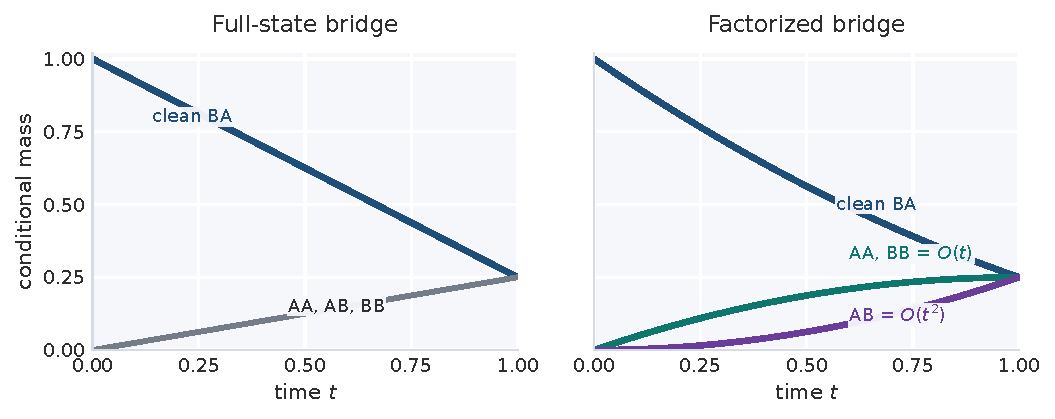
\includegraphics[width=0.92\textwidth]{figures/handouts/discrete_diffusion/fig_discrete_bridge_probabilities}
  \caption{Condition on the current bridge state \texttt{BA} in a two-token binary example.
  Under the exact full-state bridge, the alternative endpoint sequences \texttt{AA}, \texttt{AB}, and \texttt{BB} all enter at first order because one bridge time controls the whole sequence.
  Under the factorized bridge, \texttt{AA} and \texttt{BB} require one backward switch, while \texttt{AB} requires two independent switches and therefore appears only at second order.}
  \label{fig:full-vs-factorized-probabilities}
\end{figure}

This two-token toy calculation is the cleanest reason that coordinatewise marginals become sufficient after factorization.
The same distinction becomes more geometric on the two-dimensional ring example from the diffusion-models unit once we discretize the plane to a grid.
Bin the ring-mixture data law onto that grid, discretize the Gaussian reference law coordinatewise, and apply the factorized bridge \eqref{eq:factorized-mixture-path}.
At the level of marginals we still see the same kind of interpolation from the data endpoint law to the reference endpoint law.
The difference is in the sample-path geometry: the bridge no longer traces a Euclidean curve, and it instead moves by coordinatewise jumps between grid cells.

\begin{figure}[t]
  \centering
  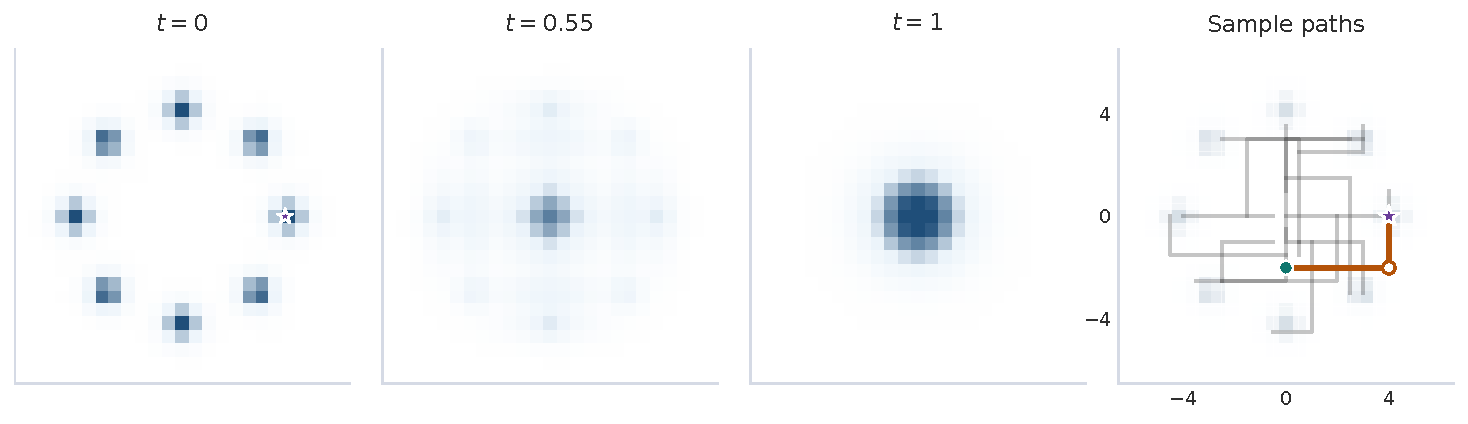
\includegraphics[width=\textwidth]{figures/handouts/discrete_diffusion/fig_discrete_spatial_bridge}
  \caption{A discretized version of the two-dimensional ring-mixture bridge.
  The first three panels show the bridge marginals on the grid at \(t=0\), \(t=0.55\), and \(t=1\).
  The last panel shows sample paths of the factorized bridge; the highlighted path starts from the starred data cell and ends at the teal reference draw.
  The marginal bridge still interpolates between the same endpoint laws, but individual paths move by one-coordinate jumps.}
  \label{fig:discrete-spatial-bridge}
\end{figure}

This is the discrete counterpart of the expectation-based picture in the continuous-state part of the diffusion-models unit.
There one learns a conditional expectation and reads off a velocity field on \(\R^2\).
Here the same bridge logic produces local jump intensities instead of a spatial vector field, which is why the finite-state description naturally passes through a generator.

For a sequence \(x\in\mathcal{V}^d\), let \(x^{j\to v}\) denote the neighbor obtained by replacing coordinate \(j\) by token \(v\).
The endpoint-conditioned generator is then as simple as possible.

\begin{proposition}[Endpoint-conditioned backward switch rule for the factorized bridge]
\label{prop:factorized-conditional-generator}
Let \(c_t\coloneqq -\dot\alpha_t/(1-\alpha_t)\), and assume \(0<\alpha_t<1\).
Then for every single-token neighbor \(x^{j\to v}\),
\begin{equation}
  Q_t^{x_0}\!\bigl(x^{j\to v}\mid x\bigr)
  =
  c_t\,\mathbf{1}\{v=x_{0,j}\}\,\mathbf{1}\{x_j\neq x_{0,j}\},
  \label{eq:factorized-conditional-generator}
\end{equation}
with diagonal chosen so that \(\sum_y Q_t^{x_0}(y\mid x)=0\).
\end{proposition}
\begin{proof}
Fix \(x_0\) and \(x\), and use the coordinatewise coupling \eqref{eq:factorized-coupling}.
If \(x_j=x_{0,j}\), then stepping backward does not require any change at coordinate \(j\).
If \(x_j\neq x_{0,j}\), conditioning on \(X_0=x_0\) and \(X_t=x\) forces \(\tau_j\le t\) and \(\Xi_j=x_j\), and the coordinate switches back exactly when \(\tau_j\in(t-h,t]\).
Therefore
\[
  \mathbb{P}(X_{t-h,j}=x_{0,j}\mid X_0=x_0,X_t=x, x_j\neq x_{0,j})
  =
  \frac{\alpha_{t-h}-\alpha_t}{1-\alpha_t}
  =
  hc_t+o(h).
\]
Independence of the switch times implies that simultaneous switches of two distinct coordinates are \(O(h^2)\), so they disappear at generator scale.
The only off-diagonal first-order moves are the backward switches in \eqref{eq:factorized-conditional-generator}.%
\end{proof}

To pass from the endpoint-conditioned generator to the marginal generator, we use the same posterior-averaging step as in the diffusion-models unit.

\begin{proposition}[Generator-level marginalization on a finite state space]
\label{prop:generator-marginalization}
Suppose
\[
  K_{t-h\mid t}(y\mid x)
  =
  \delta_x(y)+hQ_t(y\mid x)+o(h)
\]
and
\[
  K^{x_0}_{t-h\mid t}(y\mid x)
  =
  \delta_x(y)+hQ_t^{x_0}(y\mid x)+o(h)
\]
as \(h\downarrow 0\).
Then
\[
  Q_t(y\mid x)
  =
  \sum_{x_0\in S} Q_t^{x_0}(y\mid x)\,q_{0\mid t}(x_0\mid x).
\]
\end{proposition}
\begin{proof}
Apply \Cref{prop:finite-state-kernel-marginalization} with \(s=t-h\), insert the first-order expansions, subtract the common zeroth-order term \(\delta_x(y)\), divide by \(h\), and let \(h\downarrow 0\).%
\end{proof}

\begin{theorem}[Factorized generator rates depend only on coordinate marginals]
\label{thm:factorized-rates}
For the factorized mixture path \eqref{eq:factorized-mixture-path}, every off-diagonal single-token jump satisfies
\begin{equation}
  Q_t\!\bigl(x^{j\to v}\mid x\bigr)
  =
  c_t\,q_{0\mid t}\!\bigl(X_{0,j}=v\mid X_t=x\bigr),
  \qquad v\neq x_j.
  \label{eq:factorized-rate}
\end{equation}
\end{theorem}
\begin{proof}
Combine \Cref{prop:generator-marginalization} and \Cref{prop:factorized-conditional-generator}:
\[
  Q_t\!\bigl(x^{j\to v}\mid x\bigr)
  =
  \sum_{x_0\in S}
  c_t\,\mathbf{1}\{x_{0,j}=v\}\,\mathbf{1}\{x_j\neq x_{0,j}\}\,
  q_{0\mid t}(x_0\mid x).
\]
If \(v\neq x_j\), then the second indicator is automatically one on the event \(\{x_{0,j}=v\}\), so
\[
  Q_t\!\bigl(x^{j\to v}\mid x\bigr)
  =
  c_t\sum_{x_0\in S}\mathbf{1}\{x_{0,j}=v\}\,q_{0\mid t}(x_0\mid x)
  =
  c_t\,q_{0\mid t}(X_{0,j}=v\mid X_t=x).
\]
\end{proof}

If we write
\[
  \mu_{t,j}(x)\coloneqq \E[e_{X_{0,j}}\mid X_t=x]\in\R^{|\mathcal{V}|},
\]
then \Cref{thm:factorized-rates} becomes
\begin{equation}
  Q_t\!\bigl(x^{j\to v}\mid x\bigr)
  =
  c_t\,\mu_{t,j}(x)_v,
  \qquad v\neq x_j.
  \label{eq:factorized-rate-onehot}
\end{equation}
This is the cleanest statement of the simplification.
The full posterior over endpoint sequences has not disappeared.
It is still the exact posterior \(q_{0\mid t}(x_0\mid x)\) of the factorized bridge.
What the factorized bridge changes is the local move set: once only one-token backward switches are allowed at first order, the reverse rates query that posterior only through one-coordinate marginals.
So the approximation is in the bridge geometry, not in the posterior-averaging principle.
This is the generator-level reason that tokenwise classification becomes the practical training target.
The next theorem makes that precise: once the factorized bridge has been chosen, exact coordinate posteriors recover its exact reverse generator.

The full-state theorem above says that exact reverse kernels recover the correct law on any time grid.
For the factorized bridge, the parallel statement is now infinitesimal:
an ideal coordinatewise posterior model recovers the exact reverse generator of the chosen factorized bridge.
Recovering the corresponding marginal path on a time grid is then a separate numerical question, handled below by a bound in terms of accumulated one-step kernel error.

\begin{proposition}[Reverse Kolmogorov equation on a finite state space]
\label{prop:reverse-kolmogorov}
Let \(S\) be finite, let \(\pi_t\) be a differentiable path of probability mass functions on \(S\), and let \(Q_t\) be rate matrices whose entries depend continuously on \(t\).
Then the short-time relation
\[
  \pi_{t-h}(y)
  =
  \sum_{x\in S}
  \pi_t(x)\bigl[\delta_x(y)+hQ_t(y\mid x)\bigr]
  +o(h)
\]
for every \(y\in S\) is equivalent to the reverse Kolmogorov equation
\[
  -\frac{d}{dt}\pi_t(y)
  =
  \sum_{x\in S}
  \pi_t(x)\,Q_t(y\mid x),
  \qquad y\in S.
\]
Given the terminal condition \(\pi_1\), this linear ODE has a unique solution.
\end{proposition}
\begin{proof}
Because \(\sum_x \pi_t(x)\delta_x(y)=\pi_t(y)\), the short-time relation is
\[
  \pi_{t-h}(y)
  =
  \pi_t(y)
  +
  h\sum_{x\in S}\pi_t(x)\,Q_t(y\mid x)
  +
  o(h).
\]
Subtract \(\pi_t(y)\), divide by \(h\), and let \(h\downarrow 0\) to obtain the reverse Kolmogorov equation.
Conversely, if the reverse Kolmogorov equation holds, then differentiability gives
\[
  \pi_{t-h}(y)
  =
  \pi_t(y)-h\dot\pi_t(y)+o(h)
  =
  \pi_t(y)
  +
  h\sum_{x\in S}\pi_t(x)\,Q_t(y\mid x)
  +
  o(h),
\]
which is the short-time relation.
Uniqueness follows because this is a linear ODE on the finite-dimensional space \(\R^{|S|}\).%
\end{proof}

\begin{theorem}[Exact coordinate posteriors recover the factorized reverse generator]
\label{thm:factorized-infinitesimal-exactness}
For the factorized mixture path \eqref{eq:factorized-mixture-path}, suppose a model returns the exact coordinate marginals
\[
  \rho_{t,j}^\star(v\mid x)
  =
  q_{0\mid t}(X_{0,j}=v\mid X_t=x).
\]
Define the learned generator by
\[
  \hat Q_t^\star\!\bigl(x^{j\to v}\mid x\bigr)
  \coloneqq
  c_t\,\rho_{t,j}^\star(v\mid x),
  \qquad v\neq x_j,
\]
with diagonal chosen so that \(\sum_y \hat Q_t^\star(y\mid x)=0\).
Then \(\hat Q_t^\star=Q_t\), where \(Q_t\) is the exact reverse generator of the factorized bridge.
Consequently the factorized marginal path \(p_t\) is the unique solution of
\[
  -\frac{d}{dt}p_t(y)
  =
  \sum_{x\in S} p_t(x)\,\hat Q_t^\star(y\mid x),
  \qquad
  p_1 \text{ fixed},
\]
so the exact reverse CTMC for the factorized bridge transports the factorized marginal path back to \(p_0\).
\end{theorem}
\begin{proof}
The equality \(\hat Q_t^\star=Q_t\) is exactly \Cref{thm:factorized-rates}.
Because \(Q_t\) is the exact reverse generator of the factorized bridge,
\[
  K_{t-h\mid t}(y\mid x)
  =
  \delta_x(y)+hQ_t(y\mid x)+o(h).
\]
Combining this with \Cref{prop:reverse-kernels-transport} gives
\[
  p_{t-h}(y)
  =
  \sum_{x\in S}
  p_t(x)\bigl[\delta_x(y)+hQ_t(y\mid x)\bigr]
  +o(h).
\]
By \Cref{prop:reverse-kolmogorov}, the path \(p_t\) therefore solves the reverse Kolmogorov equation with generator \(Q_t=\hat Q_t^\star\).
Uniqueness gives the claim.%
\end{proof}

At this point the modeling approximation is fully visible.
The full-state sequence model and the factorized sequence model are different bridges, so they have different posteriors and different intermediate marginals.
But once the factorized bridge is chosen, \Cref{thm:factorized-infinitesimal-exactness} says that exact coordinate posteriors recover its exact reverse generator.
Equivalently, within the factorized model class the marginal dynamics are completely identified by the coordinate posteriors.
The remaining approximation is then only numerical: how accurately a discrete-time sampler tracks that reverse CTMC.

The exactness theorem above identifies the practical target immediately.
Inside the factorized bridge, learning the reverse dynamics means learning the coordinatewise posterior marginals that determine the reverse rates.
A network \(\rho_t^\theta\) therefore takes a current bridge state \(x\) and time \(t\) and outputs
\[
  \rho_{t,j}^\theta(v\mid x)
  \approx
  q_{0\mid t}(X_{0,j}=v\mid X_t=x).
\]
These outputs are still posterior objects: the full vector \(\mu_t(x)\) in the one-token case and the coordinatewise vectors \(\mu_{t,j}(x)\) in the factorized sequence case.
The statistical question is whether \(\rho_t^\theta\) learns the correct marginals.
The numerical question, which enters only after the model is trained, is how accurately a discrete-time sampler tracks the reverse CTMC determined by those marginals.
Tokenwise cross-entropy addresses the first question.

\begin{proposition}[Cross-entropy is the proper factorized objective]
\label{prop:cross-entropy-proper}
Fix \(t,x,j\), and write
\[
  \pi_j(v)\coloneqq q_{0\mid t}(X_{0,j}=v\mid X_t=x).
\]
For any candidate categorical distribution \(\rho(v)\),
\[
  \E_{V\sim \pi_j}[-\log \rho(V)]
  =
  H(\pi_j)+\operatorname{KL}(\pi_j\|\rho).
\]
Hence the expected tokenwise negative log-likelihood is minimized uniquely at \(\rho=\pi_j\).
\end{proposition}
\begin{proof}
Expand the expectation and add/subtract \(\log \pi_j(v)\):
\[
  \E_{V\sim \pi_j}[-\log \rho(V)]
  =
  \sum_v \pi_j(v)\log\frac{\pi_j(v)}{\rho(v)}
  -
  \sum_v \pi_j(v)\log \pi_j(v)
  =
  \operatorname{KL}(\pi_j\|\rho)+H(\pi_j).
\]
Only the KL term depends on \(\rho\), and it is minimized uniquely when \(\rho=\pi_j\).%
\end{proof}

The corresponding training loss is
\begin{equation}
  \mathcal{L}_{\mathrm{disc}}(\theta)
  =
  \E_{X_0\sim p_0,\; X_t\sim K_{t\mid 0}(\cdot\mid X_0),\; t\sim \mathrm{Unif}[0,1]}
  \left[
    \sum_{j=1}^d
    -\log \rho_{t,j}^\theta(X_{0,j}\mid X_t)
  \right],
  \label{eq:discrete-classification-loss}
\end{equation}
which is exactly the discrete flow-matching objective used by \citet[Eq.~(28) and Prop.~5]{gat2024discrete}.
So classification is not an extra heuristic layered on top of the bridge picture.
It is the proper scoring rule for the posterior statistics that the factorized generator actually needs.
It therefore gives the training loop directly.

\begin{algorithm}[H]
  \caption{Training a factorized discrete diffusion model}
  \label{alg:discrete-diffusion-training}
  \begin{algorithmic}[1]
    \Require Data sampler for \(p_0\), base marginals \(r_1,\dots,r_d\), schedule \(\alpha_t\), posterior network \(\rho_t^\theta\)
    \For{training steps}
      \State Sample \(x_0\sim p_0\) and \(t\sim \mathrm{Unif}[0,1]\)
      \For{\(j=1,\dots,d\) in parallel}
        \State Sample \(B_j\sim \mathrm{Bernoulli}(\alpha_t)\) and \(\Xi_j\sim r_j\)
        \If{\(B_j=1\)}
          \State Set \(x_{t,j}\gets x_{0,j}\)
        \Else
          \State Set \(x_{t,j}\gets \Xi_j\)
        \EndIf
      \EndFor
      \State Form \(x_t=(x_{t,1},\dots,x_{t,d})\)
      \State Evaluate \(\rho_{t,j}^\theta(\cdot\mid x_t)\) for all \(j\)
      \State Compute \(\ell\gets \sum_{j=1}^d -\log \rho_{t,j}^\theta(x_{0,j}\mid x_t)\)
      \State Take a gradient step on \(\ell\)
    \EndFor
  \end{algorithmic}
\end{algorithm}

Once \(\rho_t^\theta\) is trained, we obtain an approximate generator by
\[
  \hat Q_t^\theta(x^{j\to v}\mid x)
  =
  c_t\,\rho_{t,j}^\theta(v\mid x),
  \qquad v\neq x_j.
\]
An exact simulator would sample a CTMC from this generator.
For intuition, the simplest approximation is a parallel Euler step, which keeps the \(O(h)\) single-token events and ignores the \(O(h^2)\) simultaneous jumps over a step of size \(h\).

\begin{algorithm}[H]
  \caption{Euler sampling for the learned CTMC}
  \label{alg:discrete-diffusion-sampling}
  \begin{algorithmic}[1]
    \Require Base sampler for \(p_1\), time grid \(1=t_K>\cdots>t_0=0\), schedule factor \(c_t\), learned posterior network \(\rho_t^\theta\)
    \State Sample \(X_{t_K}\sim p_1\)
    \For{\(k=K,K-1,\dots,1\)}
      \State Set \(t\gets t_k\), \(h\gets t_k-t_{k-1}\), \(x\gets X_{t_k}\)
      \State Evaluate \(\rho_{t,j}^\theta(\cdot\mid x)\) for all coordinates \(j\)
      \For{\(j=1,\dots,d\) in parallel}
        \For{each \(v\neq x_j\)}
          \State \(\tilde p_j(v\mid x_j)\gets h\,c_t\,\rho_{t,j}^\theta(v\mid x)\)
        \EndFor
        \State \(\tilde p_j(x_j\mid x_j)\gets 1-h\sum_{v\neq x_j} c_t\,\rho_{t,j}^\theta(v\mid x)\)
        \State Sample \(X_{t_{k-1},j}\sim \mathrm{Categorical}(\tilde p_j(\cdot\mid x_j))\)
      \EndFor
      \State Set \(X_{t_{k-1}}\gets (X_{t_{k-1},1},\dots,X_{t_{k-1},d})\)
    \EndFor
    \State \Return \(X_{t_0}\)
  \end{algorithmic}
\end{algorithm}

Euler is only the time discretization.
The structural approximation happened earlier, when we replaced the full \(|\mathcal{V}|^d\)-state model by the factorized local bridge.
That distinction matters because classification is learning the posterior statistics needed by the chosen local generator, while Euler is only approximating the CTMC generated by those statistics.
For the per-coordinate categorical probabilities in \Cref{alg:discrete-diffusion-sampling} to be valid, we choose a grid fine enough that
\[
  h\,c_t\le 1
\]
at every step; this guarantees \(\tilde p_j(x_j\mid x_j)\ge 0\).
With that understood, the Euler sampler is one concrete family of approximate kernels \(\hat K_k\).

This isolates the remaining numerical question.
Fix a time grid and let \(K_k=K_{t_{k-1}\mid t_k}\) denote the exact reverse kernels of the factorized bridge on that grid.
Any practical sampler, including \Cref{alg:discrete-diffusion-sampling}, replaces \(K_k\) by approximate kernels \(\hat K_k\).
The only question is how those one-step kernel errors accumulate.

\begin{proposition}[Accumulated one-step kernel error controls gridwise marginal error]
\label{prop:accumulated-kernel-error}
Fix a decreasing grid \(1=t_K>\cdots>t_0=0\).
Let \(K_k=K_{t_{k-1}\mid t_k}\) be the exact reverse kernels of a bridge path, and let \(\hat K_k\) be any approximate reverse kernels on the same grid.
Start both chains from the same terminal law,
\[
  p_K=\hat p_K=p_1,
\]
and define
\[
  p_{k-1}=p_k K_k,
  \qquad
  \hat p_{k-1}=\hat p_k \hat K_k,
  \qquad k=K,\dots,1.
\]
For each step set
\[
  \varepsilon_k
  \coloneqq
  \sup_{x\in S}
  \sum_{y\in S}
  \bigl|\hat K_k(y\mid x)-K_k(y\mid x)\bigr|.
\]
Then for every \(m=0,\dots,K\),
\[
  \|\hat p_m-p_m\|_1
  \le
  \sum_{k=m+1}^K \varepsilon_k.
\]
In particular,
\[
  \|\hat p_0-p_0\|_1
  \le
  \sum_{k=1}^K \varepsilon_k.
\]
\end{proposition}
\begin{proof}
If \(m\) is any signed mass function on \(S\) and \(K\) is any Markov kernel, then
\[
  \|mK\|_1
  =
  \sum_{y\in S}
  \left|\sum_{x\in S} m(x)\,K(y\mid x)\right|
  \le
  \sum_{x\in S}|m(x)|\sum_{y\in S}K(y\mid x)
  =
  \|m\|_1.
\]
So Markov kernels are \(\ell_1\)-contractive.
Now
\[
  \hat p_{k-1}-p_{k-1}
  =
  (\hat p_k-p_k)\hat K_k
  +
  p_k(\hat K_k-K_k),
\]
and therefore
\[
  \|\hat p_{k-1}-p_{k-1}\|_1
  \le
  \|(\hat p_k-p_k)\hat K_k\|_1
  +
  \|p_k(\hat K_k-K_k)\|_1
  \le
  \|\hat p_k-p_k\|_1+\varepsilon_k.
\]
Iterating backward from \(\|\hat p_K-p_K\|_1=0\) gives the stated bound for every grid point.%
\end{proof}

\begin{corollary}[Small-step recovery of the factorized marginal path]
\label{cor:factorized-small-step-recovery}
Consider the factorized bridge \eqref{eq:factorized-mixture-path}, and suppose the learned posterior model is ideal so that \(\rho_{t,j}^\star(v\mid x)=q_{0\mid t}(X_{0,j}=v\mid X_t=x)\).
For each grid \(\Pi^{(n)}=\{1=t^{(n)}_{K_n}>\cdots>t^{(n)}_0=0\}\), let \(K_k^{(n)}\) be the exact reverse kernels of the factorized bridge and let \(\hat K_k^{(n)}\) be any approximate kernels built from those exact coordinate marginals.
If
\[
  \sum_{k=1}^{K_n}
  \sup_{x\in S}\sum_{y\in S}
  \bigl|\hat K_k^{(n)}(y\mid x)-K_k^{(n)}(y\mid x)\bigr|
  \longrightarrow 0
  \qquad\text{as } n\to\infty,
\]
then the approximate reverse chain converges at every grid point to the marginal path of the factorized bridge.
In particular,
\[
  \|\hat p_0^{(n)}-p_0\|_1\to 0.
\]
\end{corollary}
\begin{proof}
By \Cref{thm:factorized-infinitesimal-exactness}, the exact coordinate marginals recover the exact reverse generator of the factorized bridge.
Hence the exact reverse kernels \(K_k^{(n)}\) are the correct kernels for that bridge on the grid \(\Pi^{(n)}\).
Applying \Cref{prop:accumulated-kernel-error} to each grid gives the result.%
\end{proof}

This is the precise sense in which the practical factorized sampler becomes exact.
It does not say that the factorized bridge reproduces the exact full-state bridge on \(\mathcal{V}^d\); that modeling approximation was made earlier.
It says that once the factorized bridge is chosen, exact coordinate posteriors plus vanishing one-step kernel error recover its marginal path, and therefore its data endpoint \(p_0\), in the many-step limit.

\begin{exercise}[Reading factorized reverse rates]
\label{ex:reading-factorized-rates}
Stay inside the factorized bridge on the binary vocabulary \(\mathcal{V}=\{A,B\}\), and let the current bridge state be \(x=\texttt{BA}\).
Suppose
\[
  q_{0\mid t}(X_{0,1}=A\mid X_t=x)=0.6,
  \qquad
  q_{0\mid t}(X_{0,1}=B\mid X_t=x)=0.4,
\]
\[
  q_{0\mid t}(X_{0,2}=A\mid X_t=x)=0.2,
  \qquad
  q_{0\mid t}(X_{0,2}=B\mid X_t=x)=0.8,
\]
and \(c_t=3\).
\begin{enumerate}[leftmargin=*]
  \item Compute the off-diagonal reverse rates from \(\texttt{BA}\) to \(\texttt{AA}\) and to \(\texttt{BB}\).
  \item Compute the diagonal entry \(Q_t(\texttt{BA}\mid \texttt{BA})\).
  \item Explain why no table of joint probabilities \(q_{0\mid t}(X_{0,1},X_{0,2}\mid X_t=x)\) appears in these rates.
\end{enumerate}
\end{exercise}
\SolutionBox[10]{The neighbor \(\texttt{AA}\) is \(x^{1\to A}\), so \eqref{eq:factorized-rate} gives
\[
  Q_t(\texttt{AA}\mid \texttt{BA})
  =
  3\cdot q_{0\mid t}(X_{0,1}=A\mid X_t=x)
  =
  3(0.6)
  =
  1.8.
\]
Similarly \(\texttt{BB}=x^{2\to B}\), so
\[
  Q_t(\texttt{BB}\mid \texttt{BA})
  =
  3\cdot q_{0\mid t}(X_{0,2}=B\mid X_t=x)
  =
  3(0.8)
  =
  2.4.
\]
The row sum must vanish, hence
\[
  Q_t(\texttt{BA}\mid \texttt{BA})=-(1.8+2.4)=-4.2.
\]
No joint two-token table appears because the factorized bridge only allows one-token backward switches at first order.
Once the local move set is restricted to \(x^{j\to v}\), the reverse generator queries the posterior only through one-coordinate marginals.}

\begin{exercise}[Why only one-token jumps survive at first order]
\label{ex:one-token-jumps}
Use the factorized coupling \eqref{eq:factorized-coupling}.
Fix two distinct coordinates \(j\neq k\), and suppose both are currently away from their \(t=0\) endpoint values, so \(x_j\neq x_{0,j}\) and \(x_k\neq x_{0,k}\).
\begin{enumerate}[leftmargin=*]
  \item Show that
  \[
    \mathbb{P}\bigl(X_{t-h,j}=x_{0,j},\,X_{t-h,k}=x_{0,k}\mid X_0=x_0,\;X_t=x\bigr)
    =
    O(h^2).
  \]
  \item Explain why this implies that two-token jumps disappear at generator scale.
  \item Conclude that the generator-level reverse object only needs the coordinate marginals \(q_{0\mid t}(X_{0,j}=v\mid X_t=x)\), not simultaneous two-token switch probabilities.
\end{enumerate}
\end{exercise}
\SolutionBox[12]{Conditionally on \(X_0=x_0\) and \(X_t=x\), each coordinate that is away from its \(t=0\) endpoint switches back exactly when its switch time lies in \((t-h,t]\).
For one coordinate this has probability
\[
  \mathbb{P}(\tau_j\in (t-h,t]\mid \tau_j\le t)
  =
  hc_t+o(h).
\]
Because the switch times are independent across coordinates,
\begin{align*}
  &\mathbb{P}\bigl(X_{t-h,j}=x_{0,j},\,X_{t-h,k}=x_{0,k}\mid X_0=x_0,\;X_t=x\bigr) \\
  &\qquad=
  \mathbb{P}(\tau_j\in (t-h,t]\mid \tau_j\le t)\,
  \mathbb{P}(\tau_k\in (t-h,t]\mid \tau_k\le t)
  =
  \bigl(hc_t+o(h)\bigr)^2
  =
  O(h^2).
\end{align*}
After dividing by \(h\) to form the generator, any \(O(h^2)\) event vanishes.
So the first-order reverse dynamics can only move along one-token neighbors.
That is the structural reason the generator depends only on one-coordinate posterior marginals: simultaneous two-token switch probabilities never appear at first order.}

\subsection{Masked diffusion as a sharpened special case}
\label{subsec:masked-diffusion}

Masked diffusion makes the factorized story even cleaner by collapsing the reference law to a point mass.
It is not a new approximation layer; it is a particularly simple factorized bridge.
Adjoin an absorbing token \([\mathrm{MASK}]\notin\mathcal{V}\), set \(r_j=\delta_{[\mathrm{MASK}]}\) for every coordinate, and let
\[
  p_1=\delta_{[\mathrm{MASK}]^d}.
\]
Each coordinate now either keeps the \(t=0\) endpoint token or is replaced by \([\mathrm{MASK}]\).
Equivalently, the factorized bridge becomes
\begin{equation}
  K_{t\mid 0}(x\mid x_0)
  =
  \prod_{j=1}^d
  \Bigl[
    \alpha_t\,\delta_{x_{0,j}}(x_j)
    +
    (1-\alpha_t)\,\delta_{[\mathrm{MASK}]}(x_j)
  \Bigr].
  \label{eq:masked-factorized-bridge}
\end{equation}
This is the absorbing-mask version of the same factorized bridge picture.

\begin{corollary}[Revealed coordinates are already solved]
\label{cor:masked-revealed}
If \(X_{t,j}\neq [\mathrm{MASK}]\), then
\[
  q_{0\mid t}(X_{0,j}=X_{t,j}\mid X_t)=1
\]
and
\[
  q_{0\mid t}(X_{0,j}=v\mid X_t)=0
  \qquad \text{for } v\neq X_{t,j}.
\]
\end{corollary}
\begin{proof}
Under the masked bridge, a revealed token can only arise by keeping the \(t=0\) endpoint token.
So any endpoint sequence compatible with \(X_t\) must satisfy \(X_{0,j}=X_{t,j}\).%
\end{proof}

The second simplification is specific to the absorbing mask.
Once the current state tells us which coordinates are revealed and which are masked, the schedule factor contributes the same scalar weight to every compatible endpoint sequence.
After normalization it cancels.

\begin{proposition}[The masked posterior does not depend on time]
\label{prop:masked-time-independent}
Let \(x\in(\mathcal{V}\cup\{[\mathrm{MASK}]\})^d\), and define
\[
  U(x)\coloneqq \{j:x_j\neq [\mathrm{MASK}]\},
  \qquad
  M(x)\coloneqq \{j:x_j=[\mathrm{MASK}]\}.
\]
For the masked factorized bridge,
\begin{equation}
  K_{t\mid 0}(x\mid x_0)
  =
  \alpha_t^{|U(x)|}(1-\alpha_t)^{|M(x)|}
  \prod_{j\in U(x)} \mathbf{1}\{x_{0,j}=x_j\}.
  \label{eq:masked-likelihood-factor}
\end{equation}
Consequently,
\begin{equation}
  q_{0\mid t}(x_0\mid x)
  \propto
  p_0(x_0)\prod_{j\in U(x)}\mathbf{1}\{x_{0,j}=x_j\},
  \label{eq:masked-posterior-t-free}
\end{equation}
so the posterior depends on the masked pattern and the revealed tokens, but not on \(t\).
\end{proposition}
\begin{proof}
Each revealed coordinate contributes \(\alpha_t\,\mathbf{1}\{x_{0,j}=x_j\}\), and each masked coordinate contributes \(1-\alpha_t\).
Multiplying over coordinates gives \eqref{eq:masked-likelihood-factor}.
Bayes' rule then yields
\[
  q_{0\mid t}(x_0\mid x)
  \propto
  p_0(x_0)\,\alpha_t^{|U(x)|}(1-\alpha_t)^{|M(x)|}
  \prod_{j\in U(x)}\mathbf{1}\{x_{0,j}=x_j\}.
\]
The schedule factor does not depend on \(x_0\), so it cancels during normalization.%
\end{proof}

Equivalently, once we observe a masked row \(x\), the posterior is just the data law \(p_0\) renormalized on the set of endpoint sequences that agree with the revealed coordinates \(x_{U(x)}\).
The only role of the forward schedule is to contribute the common scalar \(\alpha_t^{|U(x)|}(1-\alpha_t)^{|M(x)|}\), and that scalar disappears when we normalize.

This is the posterior explanation for two familiar implementation choices.
First, the network can ignore time in the purely masked setting because the target posterior is time-independent \citep[Prop.~6 and App.~E.8]{gat2024discrete}.
Second, the loss can be restricted to masked positions because revealed coordinates already have degenerate posteriors.
That is exactly why the absorbing mask collapses the generic bridge problem to ordinary prediction on the masked coordinates.

\begin{exercise}[Why the schedule cancels in the masked case]
\label{ex:masked-cancel}
Fix a masked bridge state \(x\), and let \(U(x)\) and \(M(x)\) denote its revealed and masked coordinates.
\begin{enumerate}[leftmargin=*]
  \item Starting from \eqref{eq:masked-likelihood-factor}, show that every endpoint sequence compatible with the revealed coordinates receives the same factor
  \[
    \alpha_t^{|U(x)|}(1-\alpha_t)^{|M(x)|}.
  \]
  \item Use Bayes' rule to derive \eqref{eq:masked-posterior-t-free}.
  \item For a masked coordinate \(j\in M(x)\), prove that for every token \(v\in\mathcal{V}\),
  \[
    q_{0\mid t}(X_{0,j}=v\mid X_t=x)
    =
    \mathbb{P}_{X_0\sim p_0}\bigl(X_{0,j}=v \mid X_{0,U(x)}=x_{U(x)}\bigr).
  \]
  \item Why can the loss be restricted to masked positions?
\end{enumerate}
\end{exercise}
\SolutionBox[14]{By \eqref{eq:masked-likelihood-factor},
\[
  K_{t\mid 0}(x\mid x_0)
  =
  \alpha_t^{|U(x)|}(1-\alpha_t)^{|M(x)|}
  \prod_{i\in U(x)}\mathbf{1}\{x_{0,i}=x_i\}.
\]
So every endpoint sequence \(x_0\) compatible with the revealed coordinates gets the same schedule-dependent factor, and every incompatible sequence gets likelihood zero.
Bayes' rule gives
\[
  q_{0\mid t}(x_0\mid x)
  \propto
  p_0(x_0)\,
  \alpha_t^{|U(x)|}(1-\alpha_t)^{|M(x)|}
  \prod_{i\in U(x)}\mathbf{1}\{x_{0,i}=x_i\}.
\]
The schedule factor does not depend on \(x_0\), so it cancels during normalization:
\[
  q_{0\mid t}(x_0\mid x)
  \propto
  p_0(x_0)\prod_{i\in U(x)}\mathbf{1}\{x_{0,i}=x_i\}.
\]
Therefore, for \(j\in M(x)\),
\[
  q_{0\mid t}(X_{0,j}=v\mid X_t=x)
  =
  \mathbb{P}_{X_0\sim p_0}\bigl(X_{0,j}=v \mid X_{0,U(x)}=x_{U(x)}\bigr).
\]
Revealed positions can be dropped from the loss because their posteriors are already point masses by \Cref{cor:masked-revealed}; only the masked coordinates still carry uncertainty.}

\subsection{Connection back to the Euclidean expectation lens}
\label{subsec:euclidean-connection}

The bridge-first parallel with the Euclidean setting can be written explicitly:
\[
  \begin{aligned}
    \text{Euclidean bridge:}\qquad
    &\text{learn }
    \E[\dot X_t\mid X_t=x]
    \text{ or }
    \E[X_0\mid X_t=x].\\[0.35em]
    \text{Full finite-state bridge on }S:\qquad
    &\text{learn }
    \E[e_{X_0}\mid X_t=x]
    =
    q_{0\mid t}(\cdot\mid x).\\[0.35em]
    \text{Factorized bridge on }\mathcal{V}^d:\qquad
    &\text{learn }
    \E[e_{X_{0,j}}\mid X_t=x]
    =
    q_{0\mid t}(X_{0,j}=\cdot\mid X_t=x)
    \text{ for each }j.
  \end{aligned}
\]

The Euclidean model cannot represent the full posterior by a finite-dimensional simplex vector, so it learns the conditional expectations under that posterior that are infinitesimally sufficient for the marginal dynamics.
The one-token discrete model can represent the full posterior exactly, because a one-hot expectation on a finite set is already a probability vector.
The factorized sequence model makes the parallel tractability move: it keeps the posterior-averaging principle but chooses a local jump geometry whose infinitesimal rates depend only on coordinatewise posterior marginals.
Within that factorized model, those marginals still recover the correct reverse dynamics and therefore the correct endpoint law \(p_0\).
That is the precise sense in which practical discrete diffusion reduces to classification.

So the clean conclusion is not that discrete diffusion secretly stops being distributional.
It is the opposite.
The exact finite-state story is fully distributional from the start, and tokenwise classification appears only after we decide to approximate the full sequence model by a factorized local bridge.

\begin{exercise}[Classify the bridge]
\label{ex:classify-the-bridge}
For each scenario below, decide whether the tokenwise-classification reduction developed above is exact at the generator level, exact only in the masked/time-independent special case, or only approximate.
In each case, identify the first-order reverse move set and the first model change you would try if that reduction fails.
\begin{enumerate}[leftmargin=*]
  \item A one-token categorical bridge with a known schedule.
  \item A factorized sequence bridge with independent switch times.
  \item A masked bridge where the network is trained only on masked positions.
  \item A coupled bridge in which two-token moves occur at first order.
\end{enumerate}
\end{exercise}
\SolutionBox[14]{For the one-token categorical bridge, classification is exact at the generator level:
the reverse chain can jump from the current token \(x\) to any token \(v\neq x\), and the rates are exactly the posterior coordinates \(q_{0\mid t}(X_0=v\mid X_t=x)\).
For the factorized sequence bridge, classification is again exact at the generator level:
the first-order move set consists of one-token neighbors \(x^{j\to v}\), and the corresponding rates are exactly the coordinate marginals \(q_{0\mid t}(X_{0,j}=v\mid X_t=x)\).
For the masked bridge, this is the masked/time-independent special case of the factorized bridge, so the reduction remains exact at the generator level:
the uncertain moves live only on masked coordinates, the posterior ignores \(t\), and training can therefore be restricted to masked positions whose posteriors are not already degenerate.
For a coupled bridge with two-token moves at first order, classification is only approximate.
The reverse generator now needs block moves or other nonlocal jumps, so a tokenwise classifier is missing the first-order object itself.
The first fix is to enlarge the learned reverse object, for example by modeling blockwise posteriors or a richer reverse kernel that can score coupled edits.}

\subsection{Other discrete variants}
\label{subsec:other-discrete-variants}

The discussion above focused on one model class:
a factorized bridge, its reverse CTMC, and the discrete flow-matching objective that learns the posterior marginals needed by that generator.
That is the cleanest setup for developing the distributional picture without fragmentation.

Other named discrete diffusion models can mostly be understood as changing one of three ingredients while keeping the same bridge-first logic.
The uniform multinomial kernel of \citet[\S4]{hoogeboom2021argmax} is the basic one-token categorical instance of this story.
Absorbing-mask models are the sharpened special case from \Cref{subsec:masked-diffusion}; in discrete time this is the absorbing-state construction in \citet[\S3.1]{austin2021structured}, while in the present flow-matching setup the posterior simplification is exactly the one stated in \citep[Prop.~6 and App.~E.8]{gat2024discrete}.
Richer D3PM-style constructions play the same role by changing the one-token forward corruption kernel in the discrete-time model \citep[\S3.1--3.3]{austin2021structured}; in the bridge-first view used here, that changes the local geometry while leaving the posterior-averaging principle intact.

So the real conceptual distinction is not between many separate algorithms.
It is between the exact full-state bridge, the tractable factorized bridge, and the numerical schemes used to approximate reverse-time sampling once that bridge has been chosen.
Carried back to the main notes, the lesson is the same as in the Euclidean diffusion story: choose a bridge, identify the conditional object that is sufficient for reverse-time transport, and then ask which tractable approximation preserves that sufficiency.
The discrete setting is simply the case where, for some bridges, that conditional object is a literal posterior vector rather than a lower-dimensional summary.

\bibliographystyle{plainnat}
\makeatletter
\begingroup
\let\input@path\@empty
\IfFileExists{references.bib}{%
  \gdef\stat221bibpath{references}%
}{%
  \IfFileExists{../references.bib}{%
    \gdef\stat221bibpath{../references}%
  }{%
    \gdef\stat221bibpath{../../references}%
  }%
}
\endgroup
\makeatother
\bibliography{\stat221bibpath}

\end{document}
